% This template was originally by R. Jacob Vogelstein
% Updated on March 1, 2010 by Noah J. Cowan
% Finally put to use by Andrew Whitbeck 2013
% Copied by Christopher B Martin on Jan. 5, 2015 for use in Thesis writing

\documentclass[12pt,twoside,final]{thesis}

% FOR FINAL VERSON CHANGE TO [oneside,final]

\usepackage{mathtools}
\usepackage{setspace}
\usepackage{feynmp}
\usepackage{rotating}
\usepackage{cite}
\usepackage{amsmath,amsfonts}
\usepackage{amssymb}
\usepackage{graphicx}
\usepackage{epstopdf}
\usepackage{physics}
\usepackage{slashed}
\usepackage{hepunits}
\usepackage{SIunits}
\usepackage{mathrsfs}
\usepackage{contour}
\usepackage{color}
\usepackage{fixltx2e}
\usepackage{array}
% wrapfig is fragile: use sparingly
\usepackage{wrapfig} 
\usepackage{courier}  % Use this for ugly fonts
\usepackage[section]{placeins}

%%Added by Chris

\DeclareGraphicsRule{*}{mps}{*}{}
\usepackage{xcolor}

%My Colors
\definecolor{UniBlue}{rgb}{0.05,0.12,0.38}
\definecolor{myblue}{rgb}{0.,0.,1.}
\definecolor{myred}{rgb}{0.94,0.,0.11}
\definecolor{mygreen}{rgb}{0.13,0.44,0.07}
\definecolor{puregreen}{rgb}{0.00,1.00,0.00}
\definecolor{mygrey}{rgb}{0.39,0.39,0.39}
\definecolor{myviolet}{rgb}{0.44,0.,0.70}
\definecolor{4Lblue}{rgb}{0.47,0.67,0.88}
\definecolor{4Lgreen}{rgb}{0.33,0.54,0.33}
\definecolor{mygray}{gray}{0.30}

\definecolor{CV_Dark}{HTML}{244BFC}
\definecolor{CV_Light}{HTML}{5977FF}

\contourlength{0.5pt} %how thick each copy is
\contournumber{20}  %number of copies

%Forces figures and other floating objects to be placed within a specific subsection.
\makeatletter
\AtBeginDocument{%
  \expandafter\renewcommand\expandafter\subsection\expandafter{%
    \expandafter\@fb@secFB\subsection
  }%
}
\makeatother

%end Added by Chris


\usepackage{fancyhdr}    % Use nice looking headers along with the required footer page numbers   
%\usepackage[hypertex]{hyperref}

%Define the header/footer style
\pagestyle{fancy}
\fancyhf{}
\setlength{\headheight}{15pt}
\lhead{\leftmark}
\cfoot{\thepage}
\renewcommand{\headrulewidth}{0pt}
\fancypagestyle{plain}{% Redefine ``plain'' style for chapter boundaries
\fancyhf{} % clear all header and footer fields
\fancyfoot[C]{\thepage} % except the center
\renewcommand{\headrulewidth}{0pt}
\renewcommand{\footrulewidth}{0pt}}

%\tolerance=10000

%\makeglossary % enable the glossary

\begin{document}

\title{Characterizing a new particle using $4\ell$ events from the CMS experiment}
\author{Christopher B. Martin}
\degreemonth{July}
\degreeyear{2015} 
\dissertation
\doctorphilosophy
\copyrightnotice

% add your chaptders, best way is to have separate TeX files for each chapter
%% FRONTMATTER
\begin{frontmatter}

% generate title
\maketitle

\begin{abstract}
ABSTRACT

\vspace{.3cm}
\noindent Primary Reader: Andrei Gritsan\\
Secondary Reader:

\end{abstract}

\begin{acknowledgement}

THANKS TO

\end{acknowledgement}

%\begin{dedication} 

%\end{dedication}

% generate table of contents
\tableofcontents

% generate list of tables
\listoftables

% generate list of figures
\listoffigures

\end{frontmatter}
\chapter{Introduction}
\label{sec:intro}
\chaptermark{Introduction}

This is a sample equation:
\begin{equation}
\mathscr{L}_{EM} = \bar{\psi}\left(i\gamma^{\mu}(\partial_{\mu}+ieA_{\mu})-m\right)\psi - \frac{1}{4}F_{\mu\nu}F^{\mu\nu}.
\label{eq:EMlagrangian}
\end{equation}


This is a sample Feynman Diagram:

\begin{figure}
\begin{center}
\unitlength=1mm
\begin{fmffile}{eeScattering}

\begin{fmfgraph*}(40,30) \fmfpen{thick}
  \fmfleft{i1,i2} \fmfright{sp1,sp2}
  \fmf{fermion,label=$e^-$}{i1,v1,sp1} 
  \fmf{fermion,label=$e^-$}{i2,v2,sp2}
  \fmf{photon,label=$\gamma$}{v1,v2}
\end{fmfgraph*}

\end{fmffile}
\end{center}
\caption{Feynman diagram depicting electron-electron scattering via
the electromagnetic interaction.}
\label{fig:eeScattering}
\end{figure}

This is a sample table:

\begin{table}
\begin{center}
\begin{tabular}{l|c|c|c|c}
\hline 
\hline
particle & Q  & $T_3$ & $Y_W$ & colored \\ \hline \hline
$e_L$, $\mu_L$, $\tau_L$  & -1 & -1/2   &  -1 &  no \\ 
$e_R$, $\mu_R$, $\tau_R$  & -1 & 0      &  -2 &  no \\ 
$\nu_L$  & 0   & 1/2 & -1 & no \\ 
$u_L$, $c_L$, $b_L$    & 2/3 & 1/2  & 1/3& yes \\ 
$u_R$, $c_R$, $b_R$    & 2/3 & 0  & 4/3& yes \\ 
$d_L$, $s_L$, $t_L$    & -1/3& -1/2 & 1/3& yes \\ 
$d_R$, $s_R$, $t_R$    & -1/3& 0 & -2/3& yes \\
%H        & 0   & 1/2  & -- & no \\
%W        & 1   & 1    & -- & no \\
%Z        & 0   & --   & -- & no \\
%$\gamma$ & 0   & --   & -- & no \\
%gluon    & 0   & 0    & 0  & yes \\
\hline
\end{tabular}
\end{center}
\caption{List of SM particles and their charges. 
Q represents the charge of the $SU(1)_{em}$ gauge symmetry,
$T_3$ the broken SU(2) gauge symmetry, and $Y_W$ the broken 
U(1) gauge symmetry.}
\label{table:SMcharges}
\end{table}

\chapter{The Experiment: LHC and CMS}
\label{sec:LHC_CMS}
\chaptermark{The Experiment: LHC and CMS}

In order to answer questions about the Standard Model (SM) we need to observe processes that are extremely rare in the universe. Many measurements to test the limits of the SM can be performed by observing nature. However, to test questions about the Higgs boson, waiting for events to happen naturally would take an extremely long time\footnote{In many cases much longer than the age of the universe.}. To study these processes, labs around the world create particle colliders to generate interesting phenomenon more frequently than nature would. The rate that any physics process will occur (at a collider or otherwise) is given by the effective area of the process, \textit{cross section} $\left(\sigma\right)$, and rate those reagents pass through the same area, \textit{luminosity} $\left(\mathcal{L}\right)$; equation \eqref{eq:PhysRate}.

\begin{equation}
\label{eq:PhysRate}
\frac{d N}{dt} = \mathcal{L}\cdot\sigma
\end{equation}

The cross section for a process is the effective area of the reagents to interact in a specific way. A cross section can describe a particular number of final particles, or a specific boson used for the interaction, etc. Cross sections change depending on the energy of the interacting particles, and are usually given in units of \textit{barns} $\left(\barn = \unit{\power{10}{-24}}{\rpsquare{\centi\meter}}\right)$. They can be computed using the scattering amplitudes we have already introduced in section \ref{sec:Scattering}.

 The luminosity is a measure characterizing the source of the reagents, with units that are typically $\rpsquare{\centi\meter}\reciprocal\second$. We will discuss the particulars of this quantity for colliders, but generally luminosity is a measure of the flux of particles at a particular point in space and time.

When a particle physics experiment is designed, first numerous factors dictate what kind of particles you will accelerate and collide together. Once you have decided this, two properties define its ability to test the limits of the SM; the luminosity and the center of mass energy. With specific center of mass energies we can probe cross sections that are typically small at everyday energies. Using a higher luminosity we can increase the rate of rare events by generating interactions more often. 

\section{The Large Hadron Collider (LHC)}
\label{sec:LHC}

The Large Hadron Collider (LHC) is the largest and most powerful of these experiments in the world. It is located on the border between France and Switzerland just outside the city of Genv\`{e}ve at CERN\footnote{European Organization for Nuclear Research or Conseil Europ\'{e}en pour la Recherche Nucl\'{e}aire}. The LHC is a superconducting proton accelerator and collider measuring $\unit{27}{\kilo\meter}$ in circumference, approximately $\sim\unit{100}{\meter}$ underground. It first accelerates, then collides two beams of protons circulating the ring in opposite directions\footnote{The LHC also collides Lead ions with each other and protons, but those studies are beyond the scope of this document.}. These protons are circulated using 1232 dipole `bending' superconducting magnets and a series of other quadrupoles, sextupoles, octupoles, decapoles, etc. used for controlling and focusing the beams. The layout of the dipole magnets is shown in figure \ref{fig:LHC_Dipole} where the two beam pipes are shown along with the other magnetic, vacuum, and shielding structures.

\begin{figure}
\begin{center}
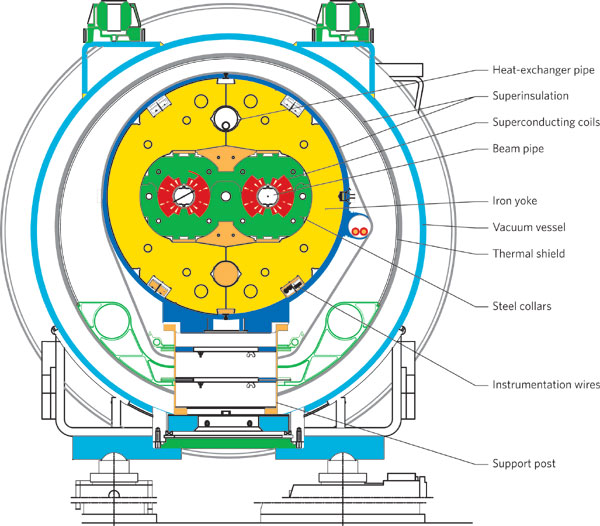
\includegraphics[width=0.65\linewidth]{{LHC_CMS/LHC_Dipole}.jpg}
\caption[A cross section schematic of the LHC Dipole magnet showing the two center beam pipes, superconducting coils (red), and other supporting structures.]{A cross section schematic of the LHC Dipole magnet showing the two center beam pipes, superconducting coils (red), and other supporting structures \cite{Bruning:782076}.}
\label{fig:LHC_Dipole}
\end{center}
\end{figure}

The LHC probes small cross sections by smashing two beams of high energy protons into each-other giving large center of mass energies. In the original design, each proton beam would have $\unit{7}{\TeV}$ of energy giving $\unit{14}{\TeV}$ in the center of mass frame. However, these studies will focus on the early years of LHC operation where the center of mass energies were $\unit{7}{\TeV}$ (2011) and $\unit{8}{\TeV}$ (2012). 

The luminosity of the LHC depends on the geometrical and electrodynamic parameters of the beam. For a beam of particles that are Gaussian distributed, the luminosity is given by the product of the beam current $\left(f_{\text{rev}}n_{b}N_{b}\right)$, brightness $\left(\frac{N_{b}}{\epsilon_{N}}\right)$, energy $\left(\frac{\gamma}{\beta^{*}}\right)$ and a geometric reduction factor $\left(F\right)$:

\begin{equation}
\label{eq:Lumi}
\mathcal{L} = \frac{1}{4\pi}\cdot\left(f_{\text{rev}}n_{b}N_{b}\right)\cdot\frac{N_{b}}{\epsilon_{N}}\cdot\frac{\gamma}{\beta^{*}}\cdot F.
\end{equation}

In this equation \eqref{eq:Lumi} the relevant factors that determine the beam current are the revolution frequency, $\left(f_{\text{rev}}\right)$, the number of proton bunches in each beam, $\left(n_{b}\right)$, and the number of protons in each bunch, $\left(N_{b}\right)$. Generally, the LHC tries to maximize this beam current so that the number of protons in each beam is as large as possible. The brightness of the beam determines how likely two protons are to interact when one bunch crosses another. It is determined by the number of protons in a bunch and the normalized transverse beam emittance, $\left(\epsilon_{n}\right)$, which is a measures of the area of the beam in the position-momentum phase space. The energy of the beam is determined by the relativistic $\gamma$ factor and the value of the beta function at the collision point, $\left(\beta^{*}\right)$. The beta function describes transverse size of the beam and $*$ denotes that this function should be evaluated at the collision point. The final term, $\left(F\right)$, is the geometrical factor that describes the reduction in luminosity because the two beams cross each-other with some non-zero angle between them. 

For the experiments that require the highest luminosities, the LHC was designed to provide $\unit{\power{10}{34}}{\rpsquare{\centi\meter}\reciprocal\second}$. The machine ran at lower luminosities for the first few years of operation as seen in the figures \ref{fig:PeakLumi} \cite{LHC_Lumi}.

\begin{figure}
\begin{center}
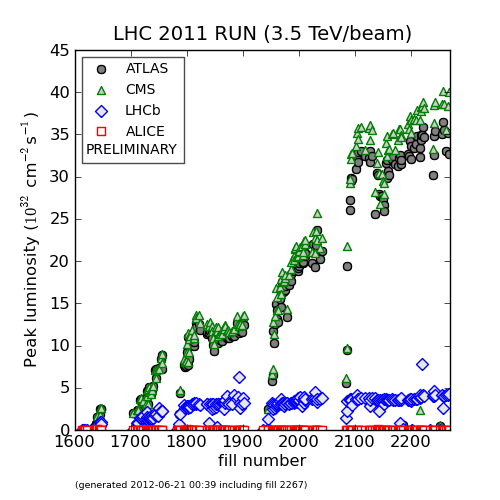
\includegraphics[width=0.45\linewidth]{{LHC_CMS/luminosity_peak_7TeV}.png}
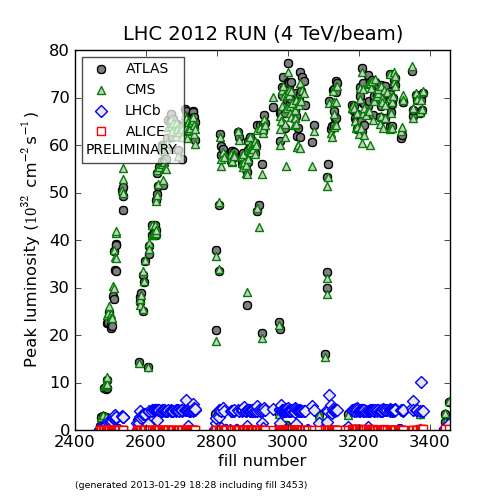
\includegraphics[width=0.45\linewidth]{{LHC_CMS/luminosity_peak_8TeV}.png}
\caption[The peak luminosity delivered to the four main LHC experiments during the 2011 $\unit{7}{\TeV}$ (left) and 2012 $\unit{8}{\TeV}$ (right) runs.]{The peak luminosity delivered to the four main LHC experiments during the 2011 $\unit{7}{\TeV}$ (left) and 2012 $\unit{8}{\TeV}$ (right) runs \cite{LHC_Lumi}.}
\label{fig:PeakLumi}
\end{center}
\end{figure}

To get the protons up to the necessary energies, protons are accelerated through a series of smaller accelerators which are pictured in figure \ref{fig:LHC}. The process starts with the $\unit{50}{\MeV}$ LINAC2 which shoots the protons into a multi-ring booster synchrotron that accelerates them up to $\unit{1.4}{\GeV}$. Next the protons are directed to the Proton Synchrotron (PS) machine which accelerates them up to $\unit{26}{\GeV}$ and generates the bunching and spacing that the LHC uses. To accelerate the beam from $\unit{26}{\GeV}$ up to $\unit{450}{\GeV}$ the beam is fed into the Super Proton Synchrotron (SPS). From the SPS the protons are fed into one of the LHC rings. Before the LHC accelerates these protons up to their final energies, this process is repeated 24 times, 12 to fill each of the two rings. Once the LHC has accelerated these proton bunches to their final energies, the beams are gradually brought together so that they will collide inside the four experiments.

\begin{figure}
\begin{center}
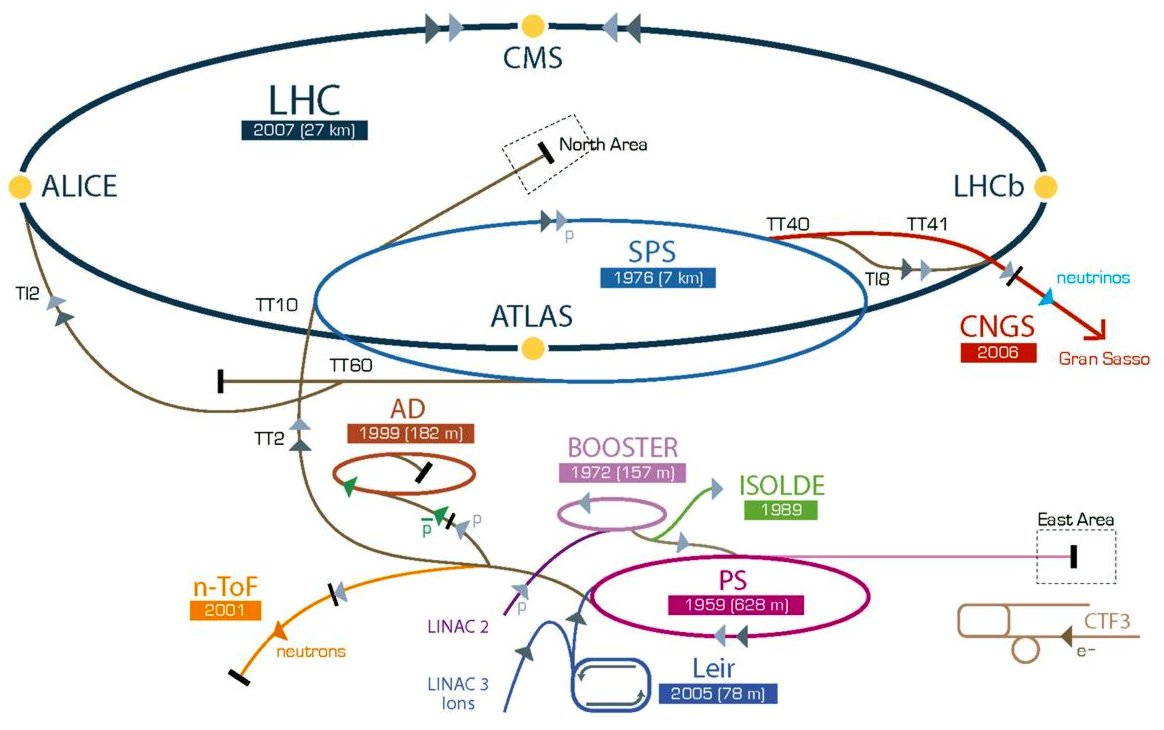
\includegraphics[width=.89\linewidth]{{LHC_CMS/LHC_nature}.jpg}
\caption[This CERN accelerator complex. Showing the full chain of accelerators used for the LHC protons: LINAC2, Booster, PS, SPS, and LHC. Additionally, the four large experiments on the LHC are shown: ALICE, ATLAS, CMS, LHCb.]{This CERN accelerator complex. Showing the full chain of accelerators used for the LHC protons: LINAC2, Booster, PS, SPS, and LHC. Additionally, the four large experiments on the LHC are shown: ALICE, ATLAS, CMS, LHCb \cite{Bruning:2007zzc}.}
\label{fig:LHC}
\end{center}
\end{figure}

The particle physics community built detectors to observe and categorize the particles that are produced when these protons (ions) are collided with each-other. Currently there are four experiments at the LHC: A Toroidal LHC ApparatuS (ATLAS), the Compact Muon Solenoid (CMS), A Large Ion Collider Experiment (ALICE), and Large Hadron Collider beauty (LHCb). The ATLAS and CMS detectors are high luminosity, multi-purpose detectors designed to test many different aspects of the SM, including the Higgs boson. LHCb looks specifically at bottom (beauty) quark interactions, while ALICE is designed for ion collisions. This work took place at the CMS experiment, described in the next sections.

\section{The Compact Muon Solenoid (CMS)}
\label{sec:CMS}

The Compact Muon Solenoid (CMS) experiment is one of the two largest experiments on the LHC. The general goal of the CMS experiment is to collect and study as many interesting events from LHC collisions as possible. To do this, CMS must identify interesting physics events and reconstruct these events as accurately as possible. At the designed energy and luminosity the LHC is expected to create $\sim 1$ billion collision events per second. It would not be possible to reconstruct all of these events, so CMS has an extensive online event selection process, called the `Trigger', that reduces this to about $100$ events per second. Some details of this process are presented in section \ref{sec:TriggerANDreconstruction}, but we will first have a discussion of the different CMS subdetectors.


To quantify how much data CMS has collected we use \textit{integrated luminosity}, which is the time integral of the luminosity, $\int \mathcal{L} dt$. This value tells experimenters how many events to expect for the specific processes they study, $N = \sigma \cdot \int \mathcal{L} dt$, and allows them to test smaller and smaller cross sections. Over the 2011 and 2012 runs\footnote{A run is a period of time denoting specific conditions for the detector or LHC.} of the CMS detector collected $\unit{5.1}{\invfb}$ and $\unit{19.7}{\invfb}$ of integrated luminosity respectively, shown in figure \ref{fig:CMSLumi}.

\begin{figure}
\begin{center}
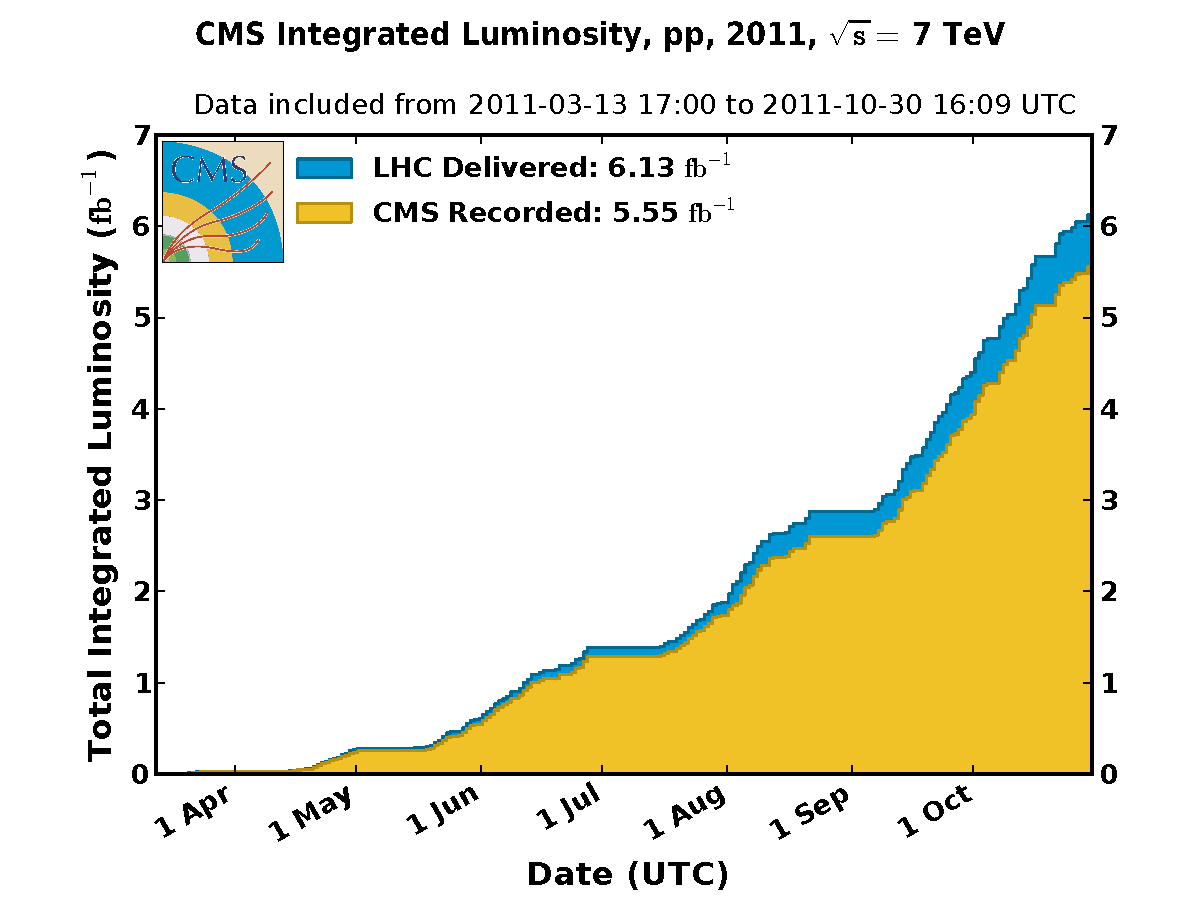
\includegraphics[width=0.45\linewidth]{{LHC_CMS/luminosity_int_7TeV}.pdf}
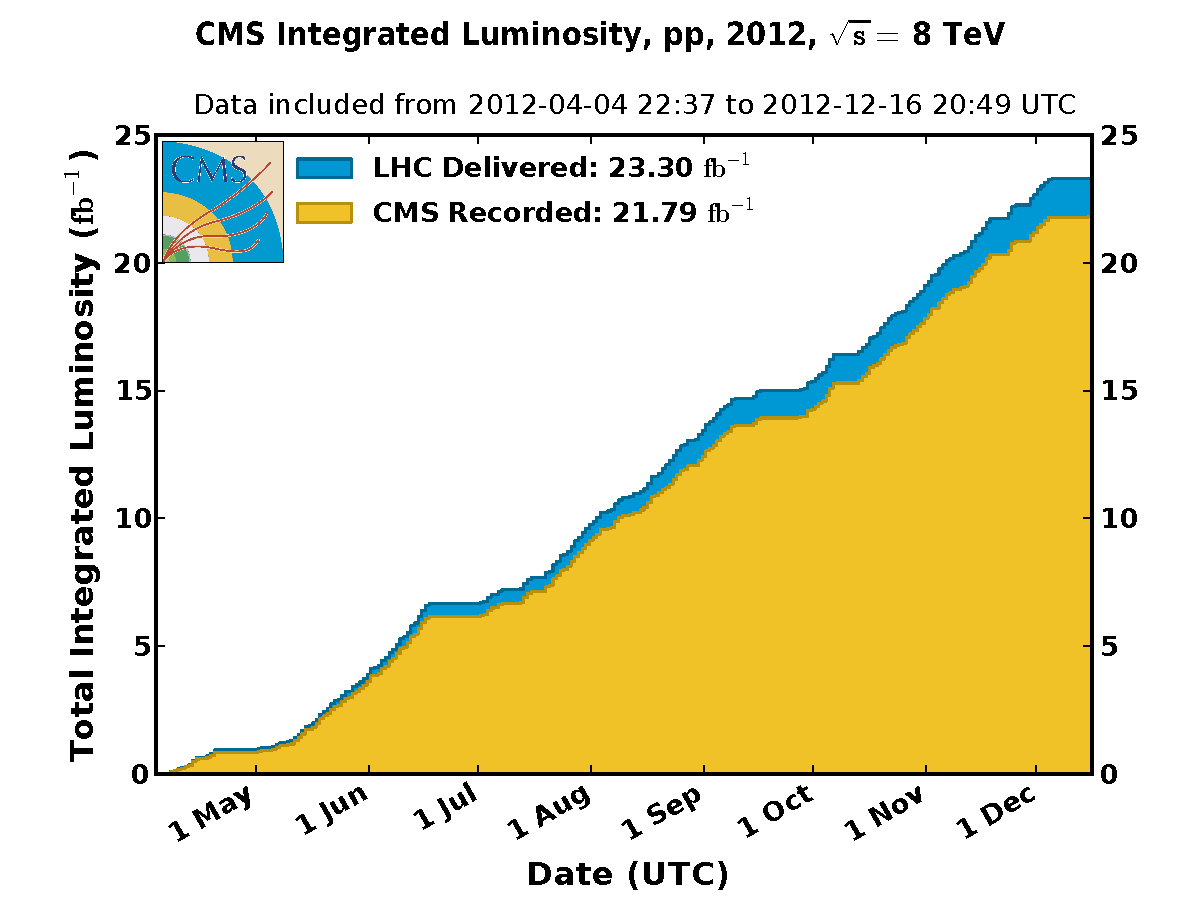
\includegraphics[width=0.45\linewidth]{{LHC_CMS/luminosity_int_8TeV}.pdf}
\caption[The integrated luminosity delivered and collected by the CMS experiment during the 2011 $\unit{7}{\TeV}$ (left) and 2012 $\unit{8}{\TeV}$ (right) runs.]{The integrated luminosity delivered and collected by the CMS experiment during the 2011 $\unit{7}{\TeV}$ (left) and 2012 $\unit{8}{\TeV}$ (right) runs, \cite{CMS_Lumi}.}
\label{fig:CMSLumi}
\end{center}
\end{figure}

To maximize the physics results that can be pulled from this data, CMS was designed with key features that give credence to its name. While it may seem oxymoronic to call a $\unit{21.6}{m}$ long and $\unit{15}{m}$ in diameter experiment `compact', the name is fitting because it is designed to put the sub-detectors within CMS close together. This compact design is a result of the $\unit{4}{\tesla}$ magnetic field that is the heart of the CMS detector. The Magnet, discussed more in section \ref{sec:Magnet}, causes the charged particles generated in collisions to bend as the flow out from the interaction point so identifying particles and measuring their momentum requires detectors that are close together. Working in concert with this field, the CMS detectors are designed to fit together as a 'cylindrical onion'. The layers of detectors and sub-detectors radiate outward from the point where the protons collisions take place. Each layer is designed to maximize the physics information that can be obtained at different distances from these collisions. The majority of the information in this section follows \cite{Bayatian:922757}.

\begin{figure}
\begin{center}
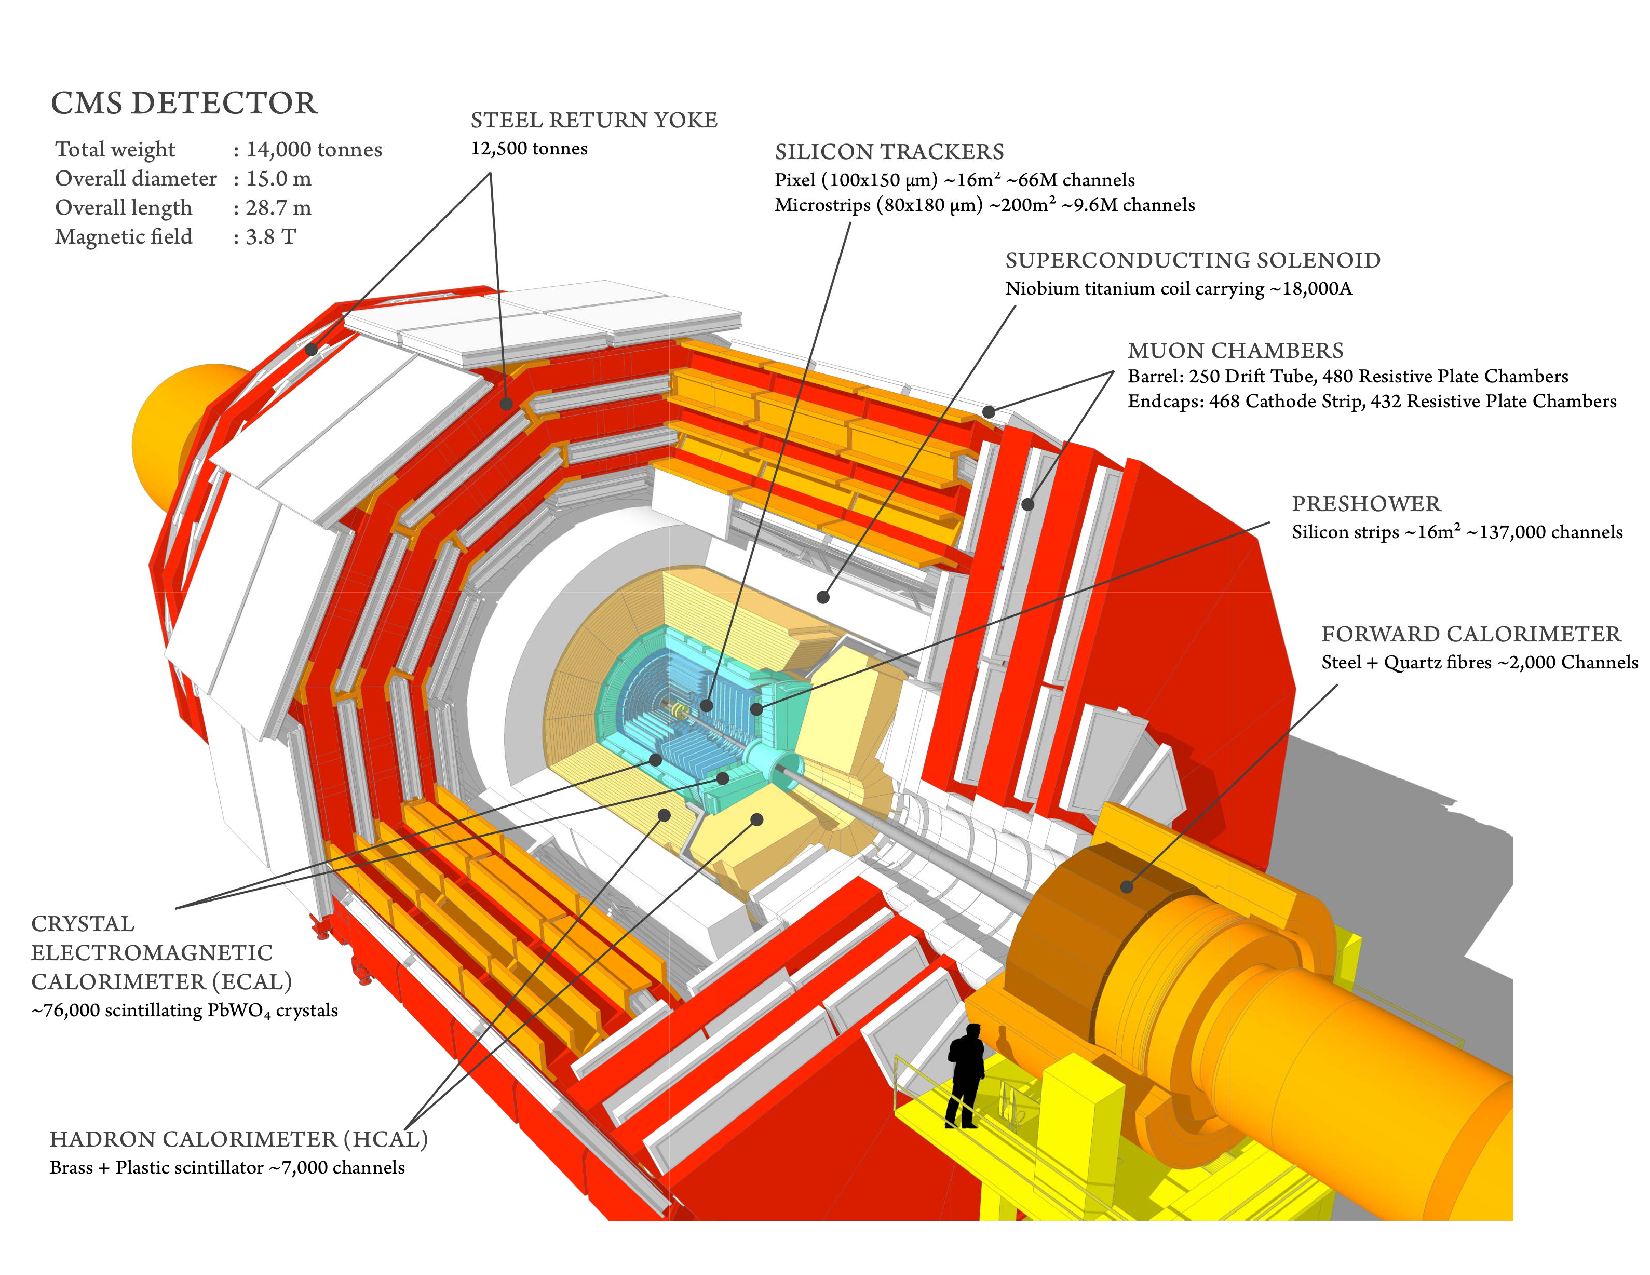
\includegraphics[width=.89\linewidth]{{LHC_CMS/cms_onion}.png}
\caption[Sectional view of the CMS detector. The LHC beams travel in opposite directions along the central axis of the CMS cylinder colliding in the middle of the CMS detector.]{Sectional view of the CMS detector. The LHC beams travel in opposite directions along the central axis of the CMS cylinder colliding in the middle of the CMS detector \cite{Sakuma:2013jqa}.}
\label{fig:CMS_onion}
\end{center}
\end{figure}

A sectional view of the CMS detectors can be seen in figure \ref{fig:CMS_onion}. From this image you can see a summary of the different subdetectors that we discuss from inside out. The innermost detector is the Silicon tracker, discussed in section \ref{sec:Tracker}, this detector is designed to give good momentum resolution for charged particles and high reconstruction efficiency requiring precise alignment of the tracking system. Additionally, this tracker needs to be able to efficiently tag $\tau$'s and b's, which will have a displaced vertex due to their long lifetimes. This requires pixel detectors close to the interaction point. 

Just outside of the tracking system is the Electromagnetic calorimeter (ECAL), discussed in section \ref{sec:ECAL}, which gives good energy and mass resolution for photons and electrons and wide geometric coverage. Further, the high segmentation of the system allows for great directional discrimination to determine the origin of the particles and to determine how isolated they are from other particles. 

The final detector that still lies inside the bore of the solenoid is the Hadronic Calorimeter (HCAL), described in section \ref{sec:HCAL}. This detector allows for accurate measurements of quark-jet mass resolution and the lateral segmentation gives directional information that is key to determine any imbalance in the transverse energy of a collision, $E_{T}^{\text{miss}}$.

Outside of the solenoid magnet lies the Muon System, described in section \ref{sec:Muon}, and the large Iron return yokes. This is the largest and heaviest part of the CMS detector\footnote{When combined with the magnet and other subdetectors the full CMS detector weighs $\sim\unit{14,000}{\text{tonnes}}$.}. This system gives good muon identification and good momentum resolution over a wide range of angles and energies for high momentum muons.

As we describe the CMS detector we will need to define a set of spacial coordinates so that we can locate ourselves within the detector. The coordinate system is defined to put the origin at the nominal collision point inside the experiment, the y-axis pointing vertically upward, the x-axis pointing along the radius of the LHC, and the z-axis pointing along the beam direction. The geometry of the detector is already cylindrical, so a modified form of cylindrical units are use for most studies. The azimuthal angle $\phi$, is given by the angle from the x-axis in the x-y plane. The polar angle, $\theta$ (from the z-axis), normally used in cylindrical coordinates, is replaced by the pseudorapidity, $\eta = -\ln\tan\left(\theta/2\right)$. The z-axis is the same as the cartesian definition. Often, interesting physics events will show distinct features in the momentum or energy transverse to the beam direction, $p_{T}$ and $E_{T}$ respectively.
 
\subsection{The Magnet}
\label{sec:Magnet}

The defining feature of CMS is the superconducting solenoid magnet, the parameters are given in table \ref{tab:CMSmagnet}. The large bending power that CMS is designed for is obtained form a reasonably-sized superconducting solenoid where the bending for charged particles starts at the primary vertex. The strong field is needed to give good momentum resolution. It bends muons tightly so that the charge is unambiguous and giving a momentum resolution of $\Delta p / p \sim 10\%$ at $p = \unit{1}{\TeVoverc}$. This design also leads to a reasonable field in the forward region where many of the detected particles will be.

\bgroup
\renewcommand{\arraystretch}{0.5}% Tighter
\begin{table}
\begin{center}
\begin{tabular}{| l | c |}
\hline 
Field & $\unit{4}{\tesla}$ \\ 
\hline 
Inner Bore & $\unit{5.9}{\meter}$ \\ 
\hline 
Length & $\unit{12.9}{\meter}$ \\ 
\hline 
Number of Turns & 2168 \\ 
\hline 
Current & $\unit{19.5}{\kilo\ampere}$ \\ 
\hline 
Stored Energy & $\unit{2.7}{\giga\joule}$ \\ 
\hline 
Hoop stress & $\unit{64}{\text{atm}}$ \\ 
\hline 
\end{tabular}
\end{center}
\caption[Parameters of the CMS superconducting solenoid.]{Parameters of the CMS superconducting solenoid, \cite{Bayatian:922757}.}
\label{tab:CMSmagnet}
\end{table}
\egroup

The magnet itself is constructed from high-purity aluminum-stabilized conductor and is indirectly cooled using a thermosiphon method.  While this type of magnet has been used at other experiments, it was a large step up in many aspects from previous magnets. To create a solenoid with the field and dimensions, a four-layer conductive winding with a large diameter wire was used so it could withstand the large outward pressure (hoop stress). The conductor carries  a $\unit{19.5}{\kilo\ampere}$ current and is co-extruded with pure and alloy aluminum to stabilize it thermally and mechanically. The conductor was manufactured in twenty continuous lengths, each of $\unit{2.65}{\kilo\meter}$. Four of these lengths were used to make each of the five coil modules within the magnet.

\begin{figure}
  \begin{center}
    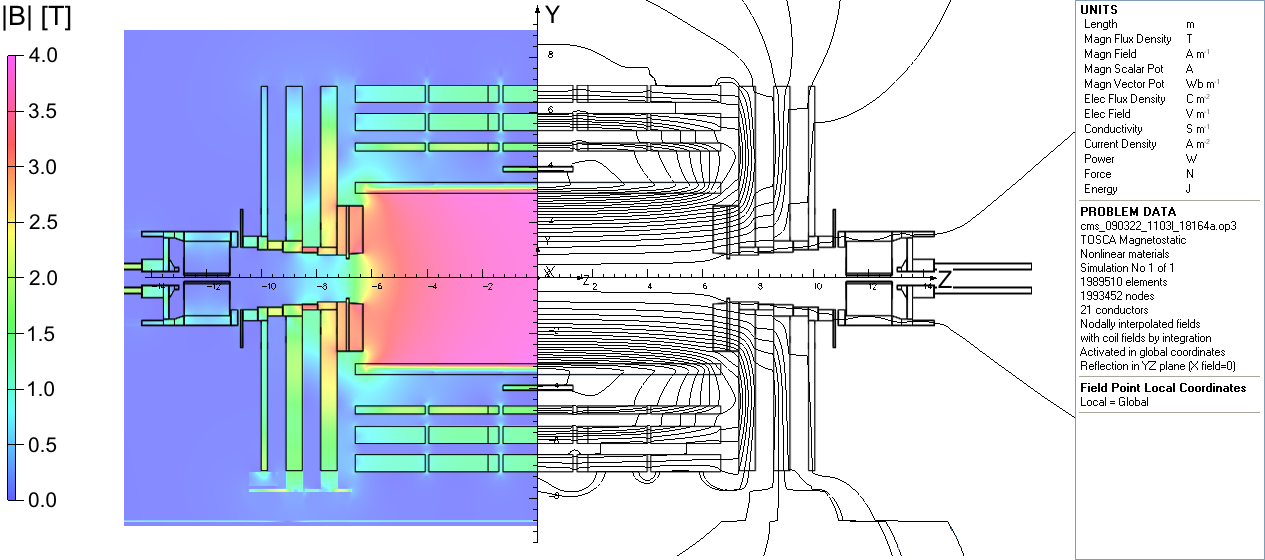
\includegraphics[width=\textwidth,trim=0 0 193 0, clip]{LHC_CMS/lines_6wb3_4_nologo.png}

    \caption[Value of magnetic field $|B|$ (left) and field lines (right) predicted on
      a longitudinal section of the CMS detector, for the underground
      model at a central magnetic flux density of 3.8~T. Each field
      line represents a magnetic flux increment of 6~Wb.]{Value of magnetic field $|B|$ (left) and field lines (right) predicted on
      a longitudinal section of the CMS detector, for the underground
      model at a central magnetic flux density of 3.8~T. Each field
      line represents a magnetic flux increment of 6~Wb \cite{Chatrchyan:2009si}.}
    \label{fig:FieldLines}
  \end{center}
\end{figure}

Working in concert with the magnet is the iron return yoke of the muon system. As can be seen in figure \ref{fig:FieldLines}, the superconducting magnet generates a large magnetic field inside the solenoid while the return flux of the field concentrates itself in the large iron structures that house the different muon detectors. These performance predictions were later confirmed by both monitors installed in the detector and with data collected from cosmic rays \cite{Chatrchyan:2009si}.

\subsection{The Inner Tracker System}
\label{sec:Tracker}

The inner tracker system is the first detector that a particle generated from an LHC collision will encounter. At the LHC, determining the origin of these particles is key and made more difficult due to the small gaps between proton bunches. The spatial resolution of the silicon tracker detector allows a particle to be mapped to the primary collision vertex (\textit{primary vertex}), secondary vertices, or identify them as \textit{pileup events}. At the designed luminosity, the LHC is expected to generate about 20 collisions\footnote{We expect more moving forward.} that will all be superimposed on an event of interest. This means that $\sim{1000}$ charged particles will appear in the detector for every interesting event. The job of the inner tracker is to measure the charge and momentum of these particles, and determine which of these originate from what vertex. To do this, the tracker has two distinct types of detectors; the 66 million \textit{silicon pixels} and 9.6 million \textit{silicon strips}. It is also vital that the positions of these detectors is accurately known at all times so that the system can operate at its ideal level. The process of determining the positions of these detectors is called \textit{Tracker Alignment} and an overview of work performed for this task is presented.

\begin{figure*}[hbtp]
  \begin{center}
    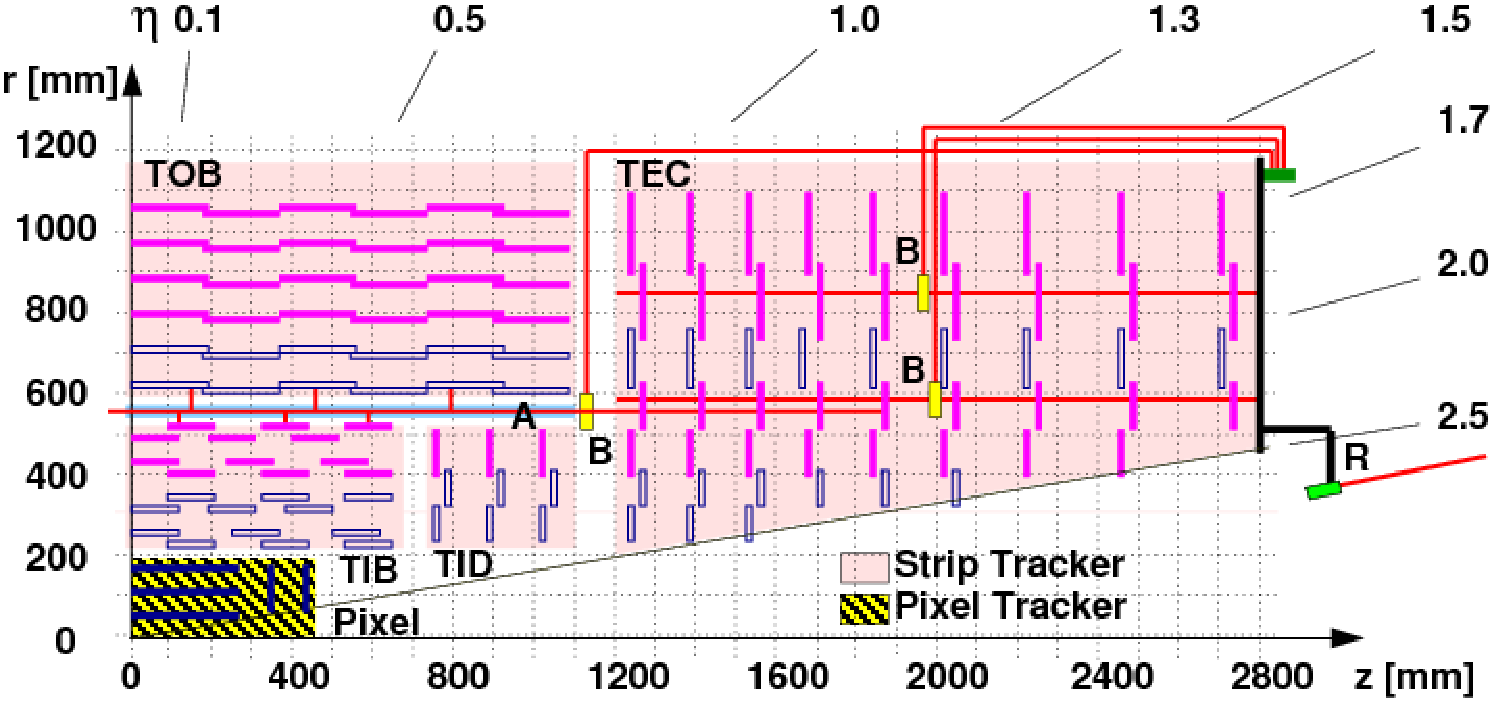
\includegraphics[width=0.7\textwidth]{{LHC_CMS/TrackerLayoutWithLAS}.pdf}
    \caption[Schematic view of one quarter of the silicon tracker in the $r$--$z$ plane.
      The positions of the pixel modules are indicated within the hatched area. At
      larger radii within the lightly shaded areas, solid rectangles represent single
      strip modules, while hollow rectangles indicate pairs of strip
      modules mounted back-to-back with a relative stereo angle.]{Schematic view of one quarter of the silicon tracker in the $r$--$z$ plane.
      The positions of the pixel modules are indicated within the hatched area. At
      larger radii within the lightly shaded areas, solid rectangles represent single
      strip modules, while hollow rectangles indicate pairs of strip
      modules mounted back-to-back with a relative stereo angle \cite{Chatrchyan:2014wfa}.}
    \label{fig:TrackerLayout}
  \end{center}
\end{figure*}

\subsubsection{Pixel Tracker}
\label{sec:Pixel}

Close to the interaction vertex the tracker consists of three layers of silicon pixel modules in the barrel region and two layers of silicon pixel modules in each forward region. The layout of the pixel detector is shown in figure \ref{fig:PixelHardware}. Each of the three barrel layers are located at radii $\unit{4.4}{\centi\meter}$, $\unit{7.3}{\centi\meter}$, and $\unit{10.2}{\centi\meter}$ from the nominal interaction point and each is $\unit{53}{\centi\meter}$ long. On either side of the three barrel layers are two end disks placed at $\abs{z} = \unit{34.5}{\centi\meter}$ and $\unit{46.5}{\centi\meter}$. 

\begin{figure}
\begin{center}
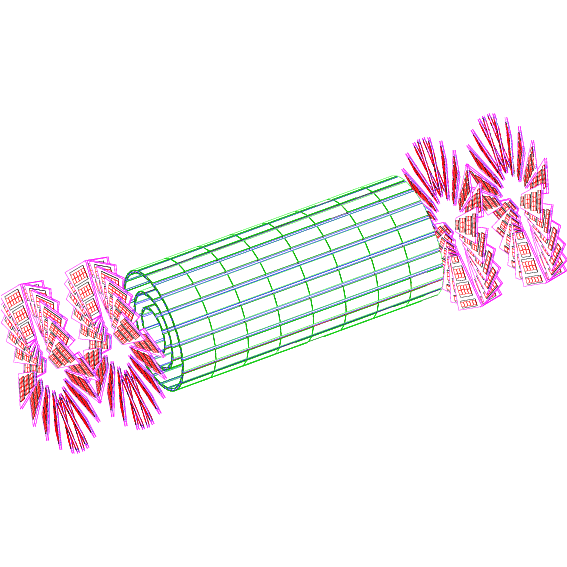
\includegraphics[width=.45\linewidth]{{LHC_CMS/PixelHardware}.pdf}
\caption[Layout of the pixel detectors in the CMS tracker.]{Layout of the pixel detectors in the CMS tracker \cite{Bayatian:922757}.}
\label{fig:PixelHardware}
\end{center}
\end{figure}

All of the pixel modules start from the same base array ($\unit{52}{\text{column}} \times \unit{80}{\text{row}}$) of pixels (size: $\unit{100}{\micro\meter} \times \unit{150}{\micro\meter}$) bump-bonded to a readout chip (ROC). Each pixel is connected to its own amplifier, shaper,  and comparator (including an individual 3-bit DAC threshold) which is connected to a `double-column' group shown in figure \ref{fig:Pixel_ROC}. The periphery of each double-column contains a data buffer, timestamp, and corresponding control and readout electronics. ROC's are grouped into modules. Each module has a different number of ROCs depending on the geometry of the region where the detectors are placed. 

\begin{figure}
\begin{center}
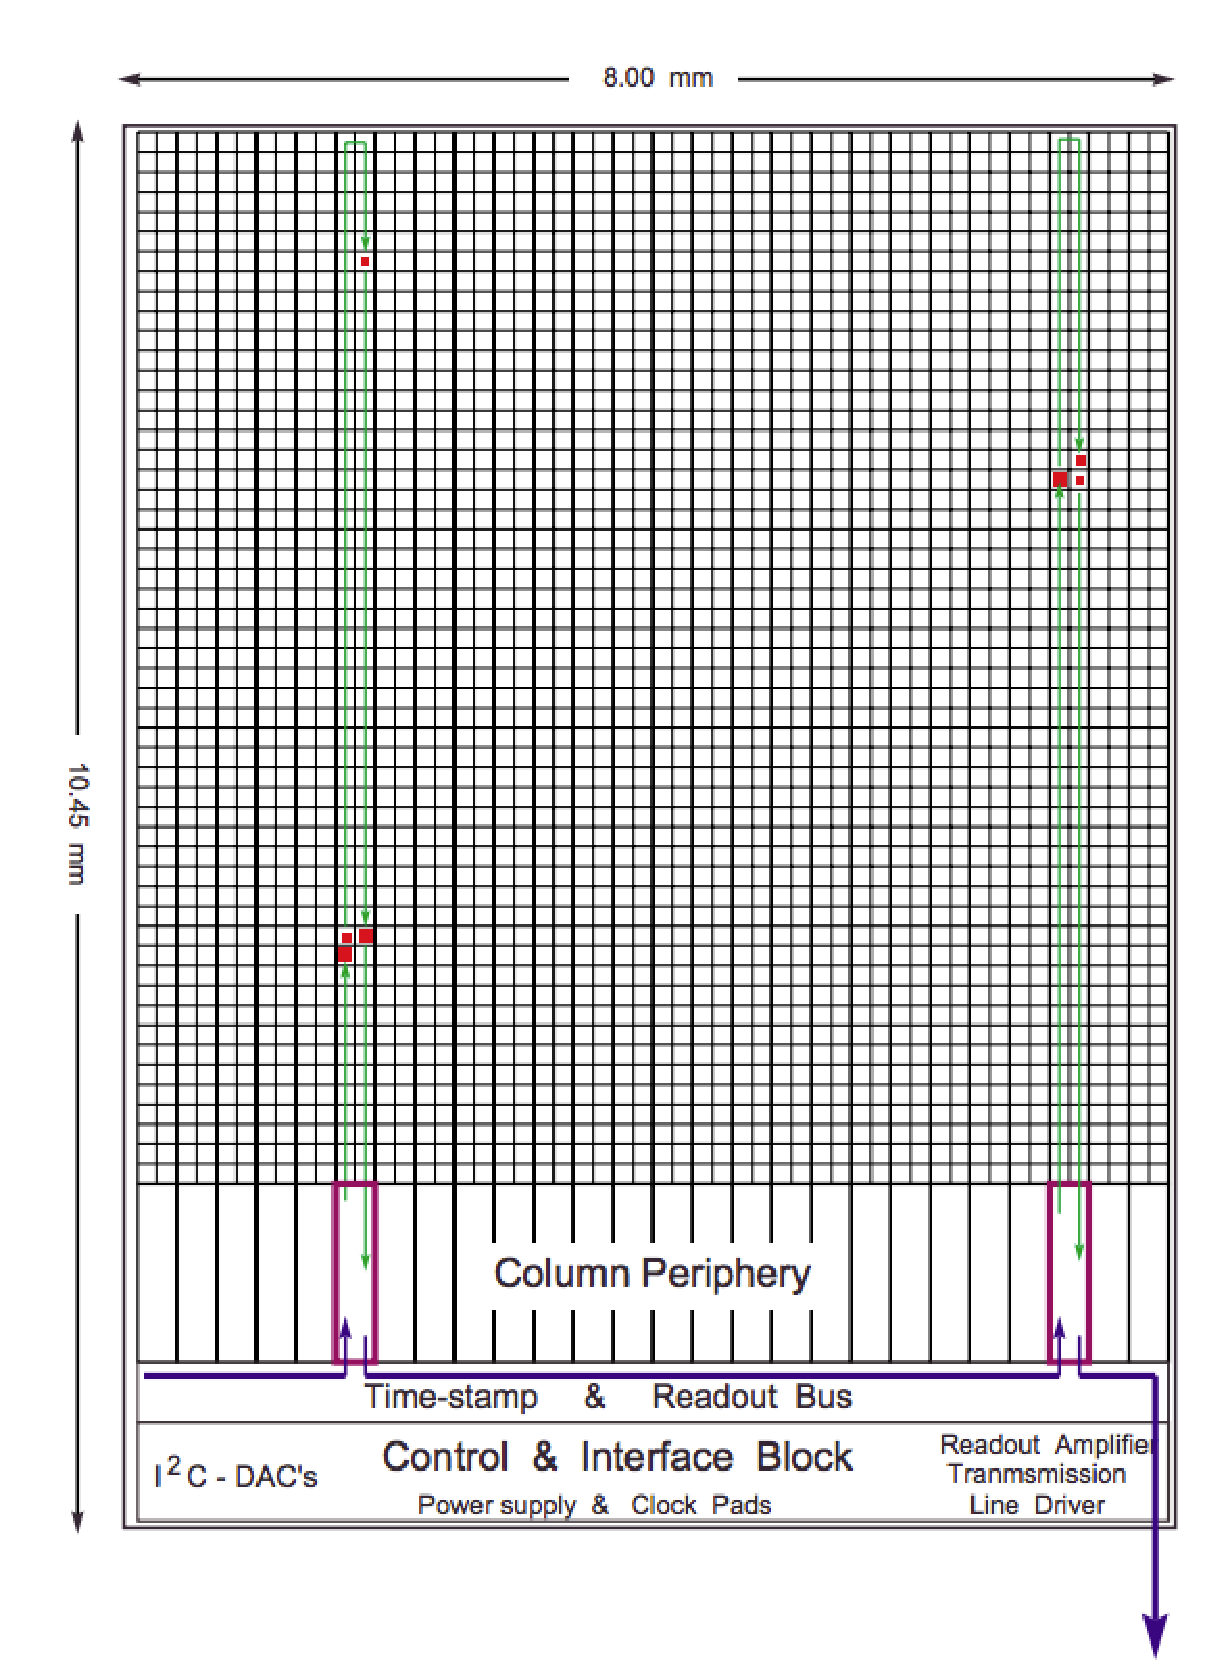
\includegraphics[width=.45\linewidth]{{LHC_CMS/Pixel_ROC}.pdf}
\caption[Layout of the pixel sensor in the CMS tracker.]{Layout of the pixel sensor in the CMS tracker \cite{Kotlinski:478252}.}
\label{fig:Pixel_ROC}
\end{center}
\end{figure}

The pixel barrel (BPIX) contains 768 modules grouped into three layers\footnote{There are smaller substructures within each layer.} and two \textit{half-barrels}\footnote{All three layers together make one half-barrel.}. While the forward pixel detectors (FPIX) are made from 672 modules grouped into two layers of turbine-like blades. The forward structures are also grouped into \textit{half-cylinders} similar to the barrel region\footnote{Again, the two layers together make the half-cylinders.}. Both the barrel layers and the blades are oriented to benefit form the large Lorentz effect (charge drift in a magnetic field) that increases the resolution through charge sharing between the pixels.

In the end, the inner tracker comprises 66 million individual pixel channels readout using approximately 16000 ROCs, giving a spatial resolution of about $\sim\unit{10}{\micro\meter}$ in $r$-$\phi$ and $\unit{20}{\micro\meter}$ in $z$. This high resolution allows for precise momentum determination for particles as they curl in the high magnetic field. It is also key to determining the origin of the particles that CMS measures. The $\sim \unit{1}{\power{\meter}{2}}$ silicon pixel detector provides coverage up to $\abs{\eta} < 2.4$.


\subsubsection{Strip Tracker}
\label{sec:Strip}

Much larger than the  pixel tracker is the $\sim \unit{200}{\power{\meter}{2}}$ silicon strip tracker. The strip tracker is divided into four parts: TIB (tracker inner barrel), TID (tracker inner disks),  TOB (tracker outer barrel), and TEC (tracker end cap). The CMS tracker is the largest silicon detector ever built. Different regions of the strip tracking system have different module types summarized in table \ref{tab:Strips}. All together, the Silicon Strip Tracker has complete coverage up to $\abs{\eta} < 2.4$.

\bgroup
\renewcommand{\arraystretch}{0.5}% Tighter
\begin{table}
\begin{center}
\begin{tabular}{ l | r | r | r }
\hline 
part & No. detectors & thickness $\left(\micro\meter\right)$ & mean pitch $\left(\micro\meter\right)$\\ 
\hline 
TIB & 2724 & 320 & 81/118 \\
TOB & 5208 & 500 & 81/183 \\
TID & 816 & 320 & 97/128/143 \\
TEC(inner) & 2512 & 320 & 96/126/128/143 \\
TEC(outer) & 3888 & 500 & 143/158/183 \\
\hline 
\end{tabular}
\end{center}
\caption[Detector types in the silicon strip tracker.]{Detector types in the silicon strip tracker, \cite{Bayatian:922757}.}
\label{tab:Strips}
\end{table}
\egroup

In the barrel region the coverage for the TIB and TOB is very different. The TIB has four layers and covers $\abs{z} < \unit{65}{\centi\meter}$ with silicon sensor of a thickness of $\unit{320}{\micro\meter}$. The first two layers are made with ``stereo" modules in order to provide both $r$-$\phi$ and $r$-$z$ measurements. These stereo modules are made with a stereo angle of $\unit{100}{\milli\radian}$ giving the TIB single-point resolution of $23$-$\unit{34}{\micro\meter}$ in $r$-$\phi$ and $\unit{23}{\micro\meter}$ in $z$. The TOB has six layers covering $\abs{z} < \unit{110}{\centi\meter}$ with silicon sensor of a thickness of $\unit{500}{\micro\meter}$. The first two layers of the TOB are also stereo modules with a stereo angle of $\unit{100}{\milli\radian}$. This gives the whole TOB a resolution of $35$-$\unit{52}{\micro\meter}$ in $r$-$\phi$ and $\unit{52}{\micro\meter}$ in $z$.

The each of the two TECs comprises nine disks that cover the $\unit{120}{\centi\meter} < \abs{z} < \unit{280}{\centi\meter}$ forward region. While the TID covers the gap between the TIB and the TEC. Both the TID and TEC modules are arranged in rings centered at the beam line. The strips in these sensors radiate outward from the beam line so the pitch is different for each strip. The first two rings of the TID and the first, second, and fifth rings of the TEC are stereo modules as well allowing for more precise resolution. The TID and first three rings for the TEC have $\unit{320}{\micro\meter}$ sensors while the rest of the TEC has $\unit{500}{\micro\meter}$ sensors.

All of these structures (BPIX, FPIX, TIB, TOB, TID, TEC) are mounted in carbon-fiber structures and are cooled to ensure they operate correctly for a long time\footnote{Because of technical problems during run 1 the detectors were not kept as cold as originally designed.}. Using the precise position information that the tracker provides CMS is able to determine with very high confidence the momentum and impact parameter (How close a particle's path is the the origin.) of particles, see figure \ref{fig:TrackerResolution}. Careful consideration is taken when these detectors are moved and installed but precise determination of the exact location of all components is key to keep the optimal resolution of these detectors. This process is not only vital during the LHC startup but care needs to be taken as the detector takes data to ensure no loss in performance.

\begin{figure}
\begin{center}
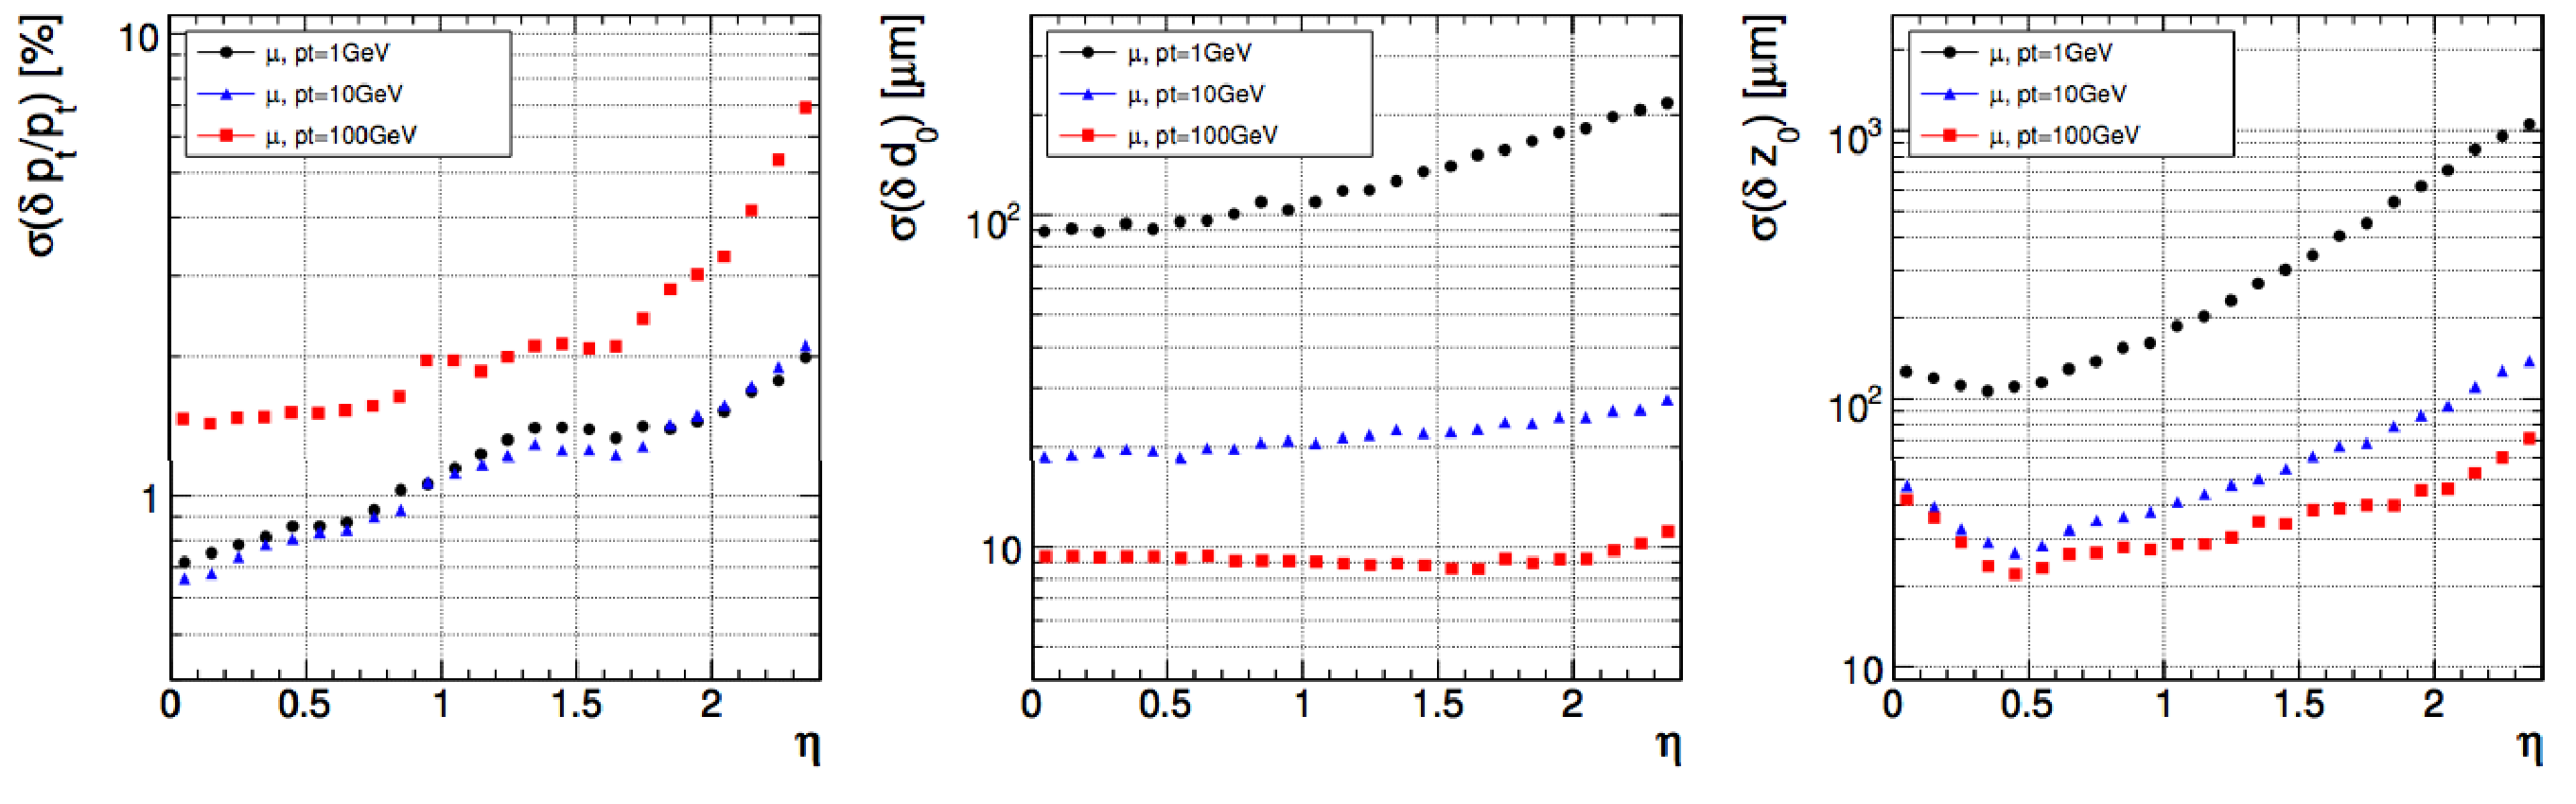
\includegraphics[width=.95\linewidth]{{LHC_CMS/TrackerResolution}.pdf}
\caption[Predicted resolution of several track parameters for single muons with $1$, $10$, and $\unit{100}{\GeV}$: transverse momentum (left), transverse impact parameter (center), and longitudinal impact parameter (right).]{Predicted resolution of several track parameters for single muons with $1$, $10$, and $\unit{100}{\GeV}$: transverse momentum (left), transverse impact parameter (center), and longitudinal impact parameter (right). \cite{Chatrchyan:1129810}.}
\label{fig:TrackerResolution}
\end{center}
\end{figure}

\subsection{Electromagnetic Calorimeter}
\label{sec:ECAL}

The CMS Electromagnetic Calorimeter (ECAL) is composed of $61200$ lead tungstate $\left(\mathrm{PbWO_{4}}\right)$ crystals mounted in the barrel part of the detector and $7324$ crystals in each of the two end caps. Together the barrel and end caps make a homogeneous and hermetic scintillating layer surrounding the Inner Tracker. The crystals were chosen to have short radiation and Moliere lengths while being fast radiation hard scintillators. Due to the low light yield of the crystal, silicon avalanche photo diodes (barrel) or vacuum phototriodes (end cap) are used because they can operate in the magnetic field. Additionally, to stabilize the response of the crystals and photo diodes a cooling system is used to maintain temperature stability. Thus, the ECAL is a compact calorimeter that is fast, has fine granularity, and is radiation resistant.

\begin{figure}
\begin{center}
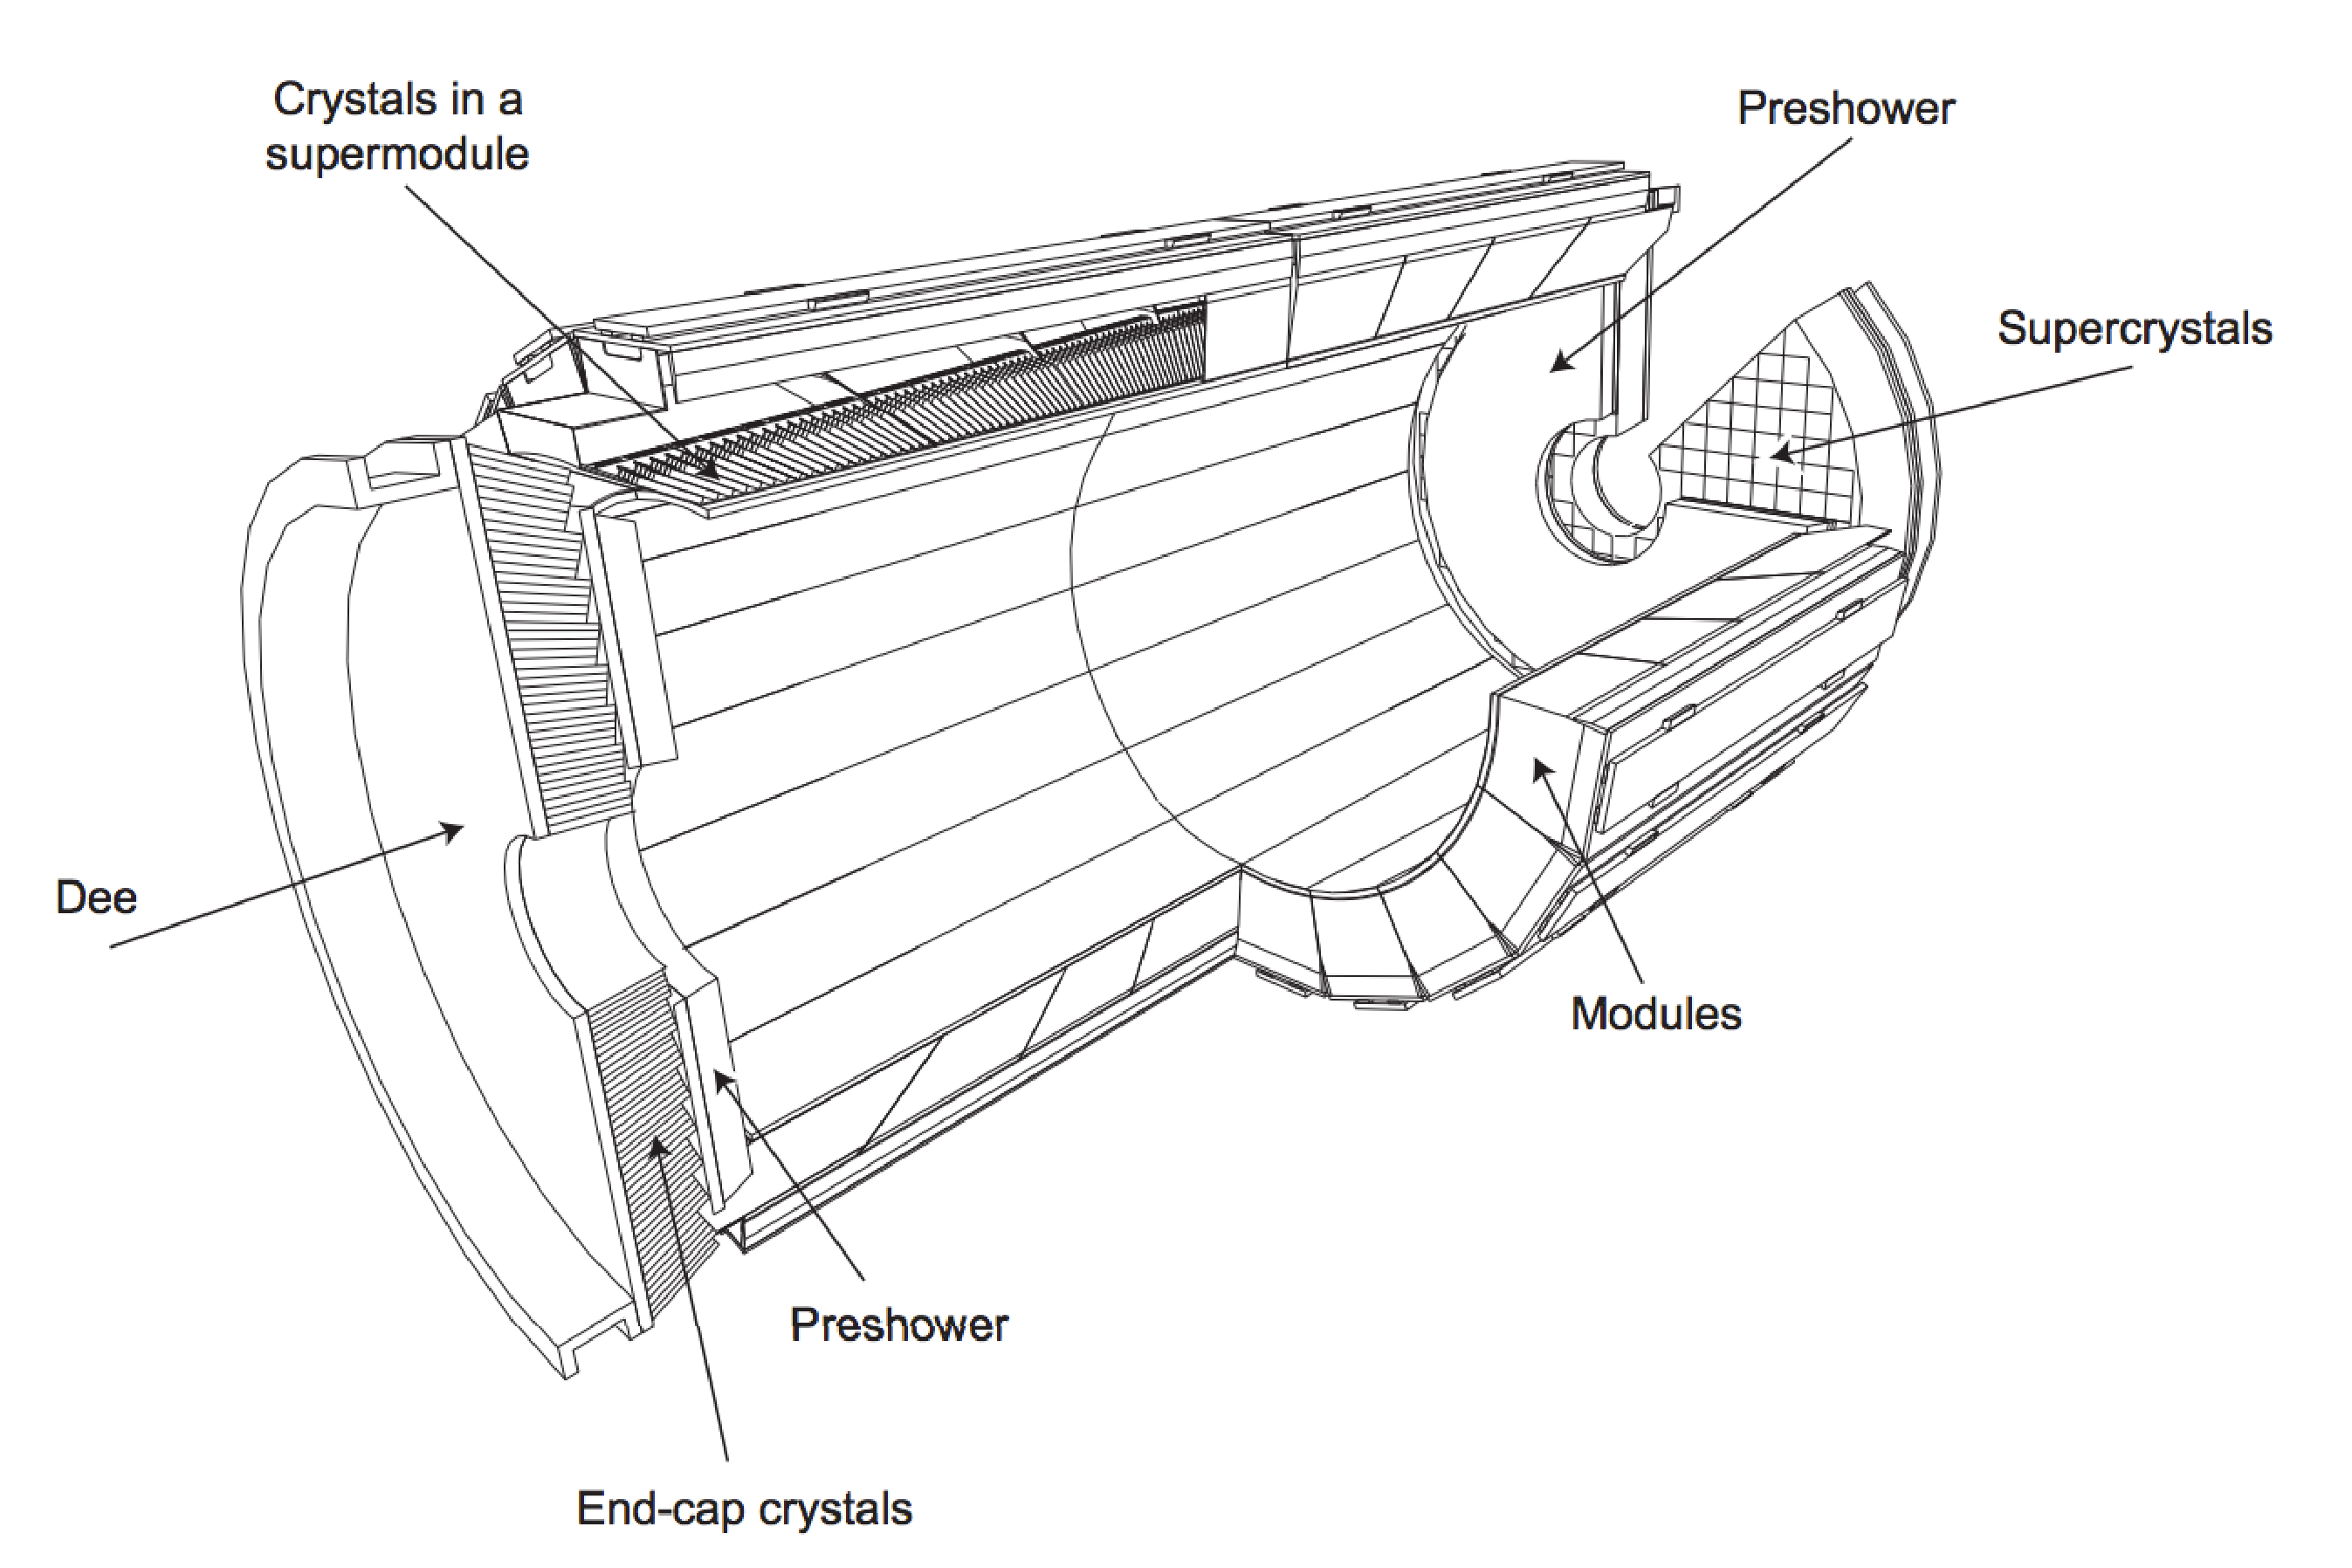
\includegraphics[width=.95\linewidth]{{LHC_CMS/CMSecal}.pdf}
\caption[Layout of the CMS electromagnetic calorimeter showing the arrangement of crystal modules, supermodules and end caps, with the preshower in front.]{Layout of the CMS electromagnetic calorimeter showing the arrangement of crystal modules, supermodules and end caps, with the preshower in front. \cite{Chatrchyan:1129810}.}
\label{fig:CMSecal}
\end{center}
\end{figure}

The ECAL barrel section (EB) has an inner radius of $\unit{129}{\centi\meter}$ and constructed as 36 identical ``supermodules" each covering half the barrel length and covering a range of $0 < \abs{\eta} < 1.479$. The crystals are installed to be quasi-projective (axis tilted $\unit{3}{\degree}$) to the nominal vertex arranged in an $\eta$-$\phi$ grid. They have a front face cross-section of $22\times\unit{22}{\power{\meter}{2}}$ and a length of $\unit{230}{\milli\meter}$.

The ECAL end caps (EE) lie at a distance of $\unit{314}{\centi\meter}$ from the vertex and cover a range of  $1.479 < \abs{\eta} < 3.0$. The end cap crystals, like the barrel, are off-point from the nominal vertex but are arranged in an $x$-$y$ grid. They have a larger face size than the barrel crystals, $28.6\times\unit{28.6}{\power{\meter}{2}}$ and a length of $\unit{220}{\milli\meter}$. Additionally, a preshower detector is placed in front of the EE consisting of two planes of silicon strip detectors each placed behind a layer of lead absorber disks. 

While the specifics of particle reconstruction are discussed in section \ref{sec:TriggerANDreconstruction}, figure \ref{fig:ECALresolution} shows the electron resolution of the EB system compared to and then combined with the inner tracker system.

\begin{figure}
\begin{center}
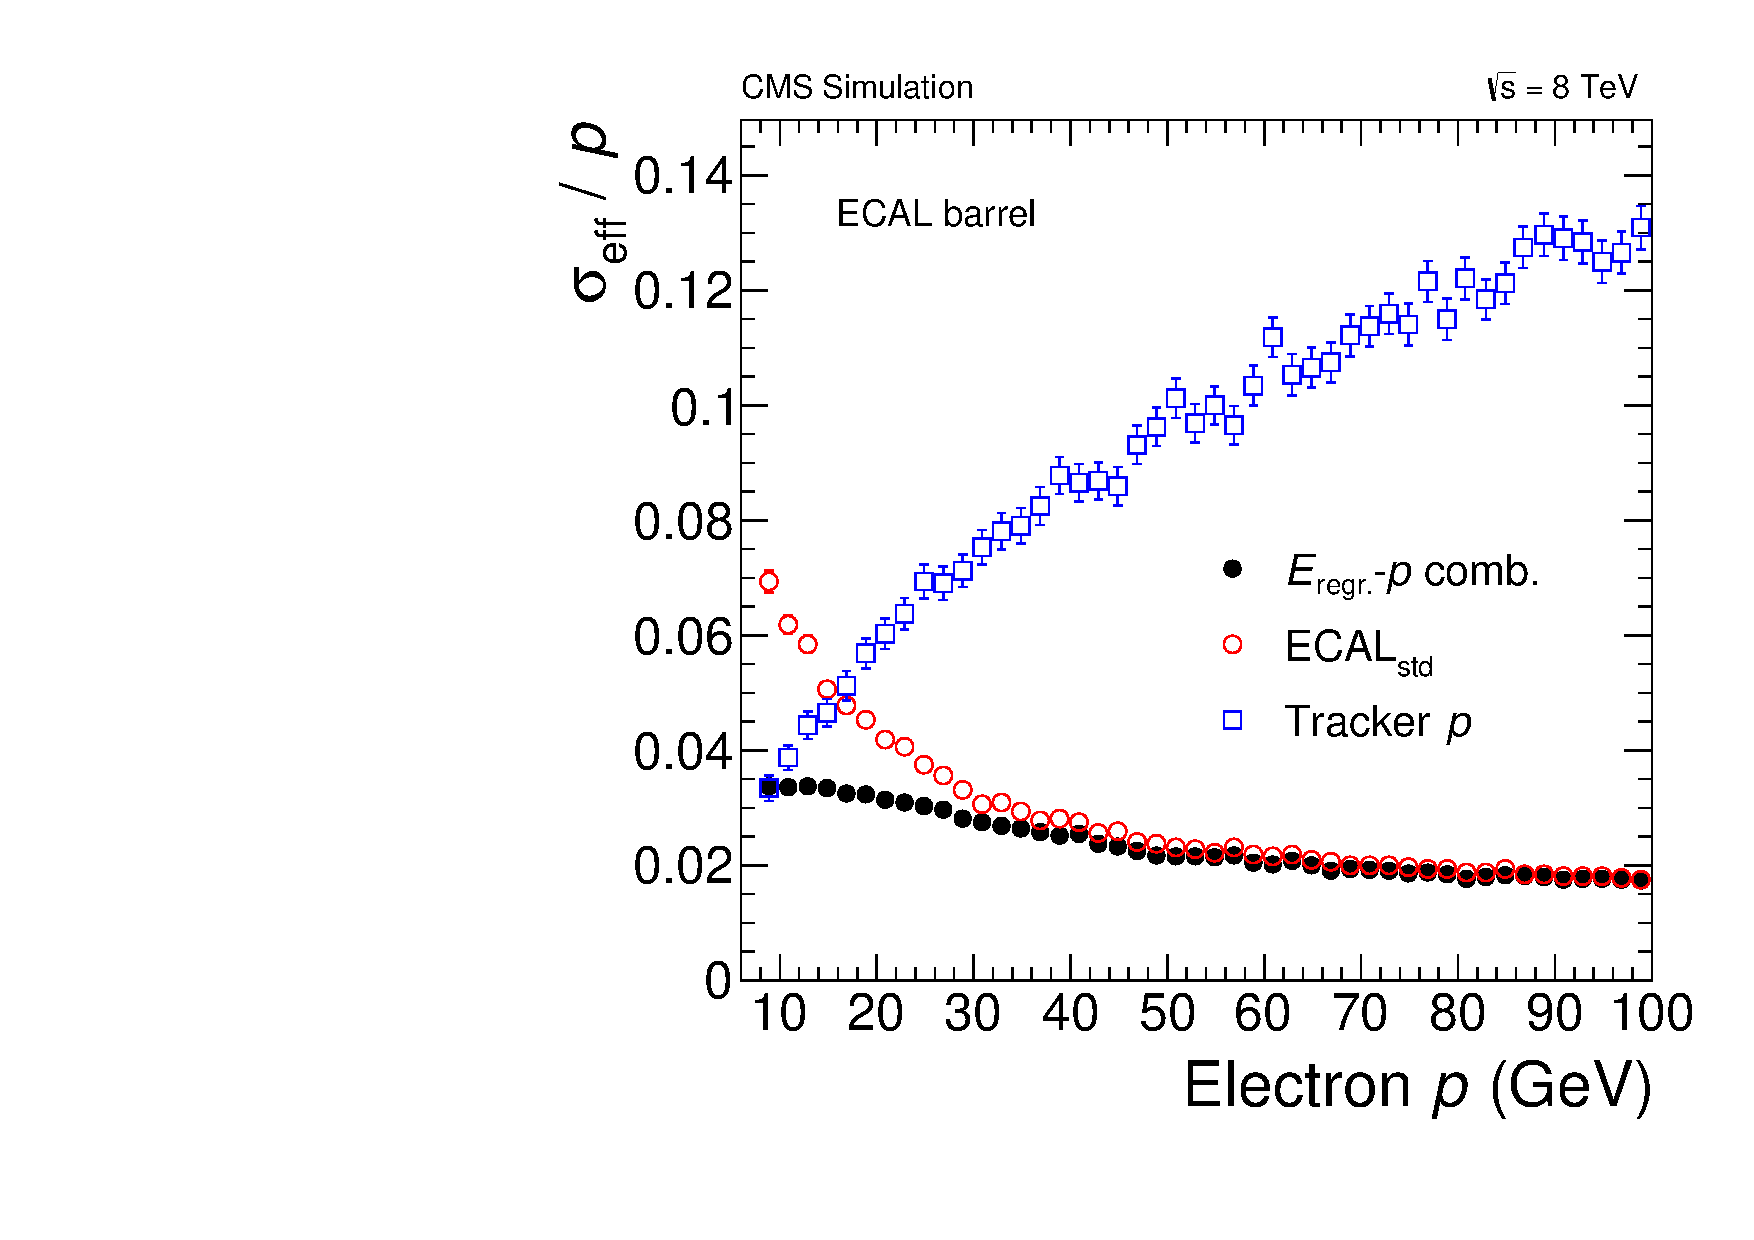
\includegraphics[width=.45\linewidth]{{LHC_CMS/effRMSbarrel_withregression_new}.pdf}
\caption[Effective momentum resolution $\sigma_{\text{eff}}/p$ for electrons in the EB as a function of the momentum for the ECAL-only, the tracker-only, and the combined estimates.]{Effective momentum resolution $\sigma_{\text{eff}}/p$ for electrons in the EB as a function of the momentum for the ECAL-only, the tracker-only, and the combined estimates. \cite{Chatrchyan:2013mxa}.}
\label{fig:ECALresolution}
\end{center}
\end{figure}

\subsection{Hadronic Calorimeter}
\label{sec:HCAL}

The design of the hadron calorimeter (HCAL) is strongly influenced by the choice of magnet parameters because most of the system is located inside the magnet coil and surrounds the ECAL system\cite{Bayatian:922757}. The HCAL system consists of a set of sampling calorimeters. The barrel (HB) and endcap (HE) calorimeters utilize alternating layers of brass as absorber and plastic scintillator as active material. The scintillation light is converted by wavelength-shifting fibers embedded in the scintillator and channeled to hybrid photodiode detectors via clear fibers. The outer calorimeter (HO) uses the CMS magnet and return yoke as the absorber while using the same active material and readout system as HB and HE. The HO system serves as a ``tail-catcher" after the magnet oil, thus reducing the tails in the energy resolution function.

The HCAL is segmented into individual calorimeter cells along three coordinates, $\eta$, $\phi$, and depth. The depth is an integer coordinate that enumerates the segmentation longitudinally, along the direction from the venter of the nominal interaction region. The layout of the system can be seen in figure \ref{fig:HCAL}. The HB system covers the region $-1.4 < \eta < 1.4$ constructed in 2 half barrels. The HE covers the region $1.3 < \abs{\eta} < 3.0$, the segmentation is not uniform in order to maintain coverage and resolution. 

\begin{figure}
\begin{center}
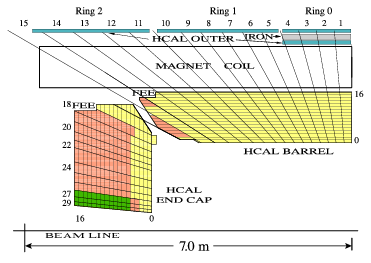
\includegraphics[width=.75\linewidth]{{LHC_CMS/HCALdiagram}.png}
\caption[A quarter slice of the CMS HCAL detectors. The right end of the beam line is the interaction point, HF (not pictured) would be located far to the left. In the diagram, the numbers on the top and left refer to segments in $\eta$, and the numbers on the right and the bottom refer to depth. Colors/shades indicate the combinations of layers that form the different depth segments, which are numbered sequentially starting at 1, moving outward from the interaction point. The outer calorimeter is assigned depth 4. Segmentation along $\phi$ is not shown.]{A quarter slice of the CMS HCAL detectors. The right end of the beam line is the interaction point, HF (not pictured) would be located far to the left. In the diagram, the numbers on the top and left refer to segments in $\eta$, and the numbers on the right and the bottom refer to depth. Colors/shades indicate the combinations of layers that form the different depth segments, which are numbered sequentially starting at 1, moving outward from the interaction point. The outer calorimeter is assigned depth 4. Segmentation along $\phi$ is not shown \cite{Chatrchyan:2009hw}.}
\label{fig:HCAL}
\end{center}
\end{figure}

Coverage between $3.0 < \abs{\eta} < 5.0$ is provided by the steel/quartz fiber hadron forward (HF) calorimeter. HF is unique in that it preferentially samples the neutral component of the hadron shower. This design leads to narrower showers and hence is ideally suited for the congested environment of the forward region. The HF detector is located outside of the muon system, $\unit{11.2}{\meter}$ from the interaction point. Unlike the scintillator that is used in the other HCAL systems, HF uses Cerenkov light emitted in the quartz fibers lay parallel to the beam and are placed in a square grid inside steel plates.

What is actually measured by the HCAL system are particle jets. This is a result of the QCD that was discussed in previous sections and is outlined a bit more in section \ref{sec:TriggerANDreconstruction}. The granularity and sampling of the different components of the HCAL system have been chosen so that the jet energy resolution is similar in all three regions (HB, HE, HF). This is illustrated in figure \ref{fig:HCALresolution} where the jet energy resolution is plotted as a function of the transverse energy. More details on this plot can be found in \cite{Bayatian:922757}.

\begin{figure}
\begin{center}
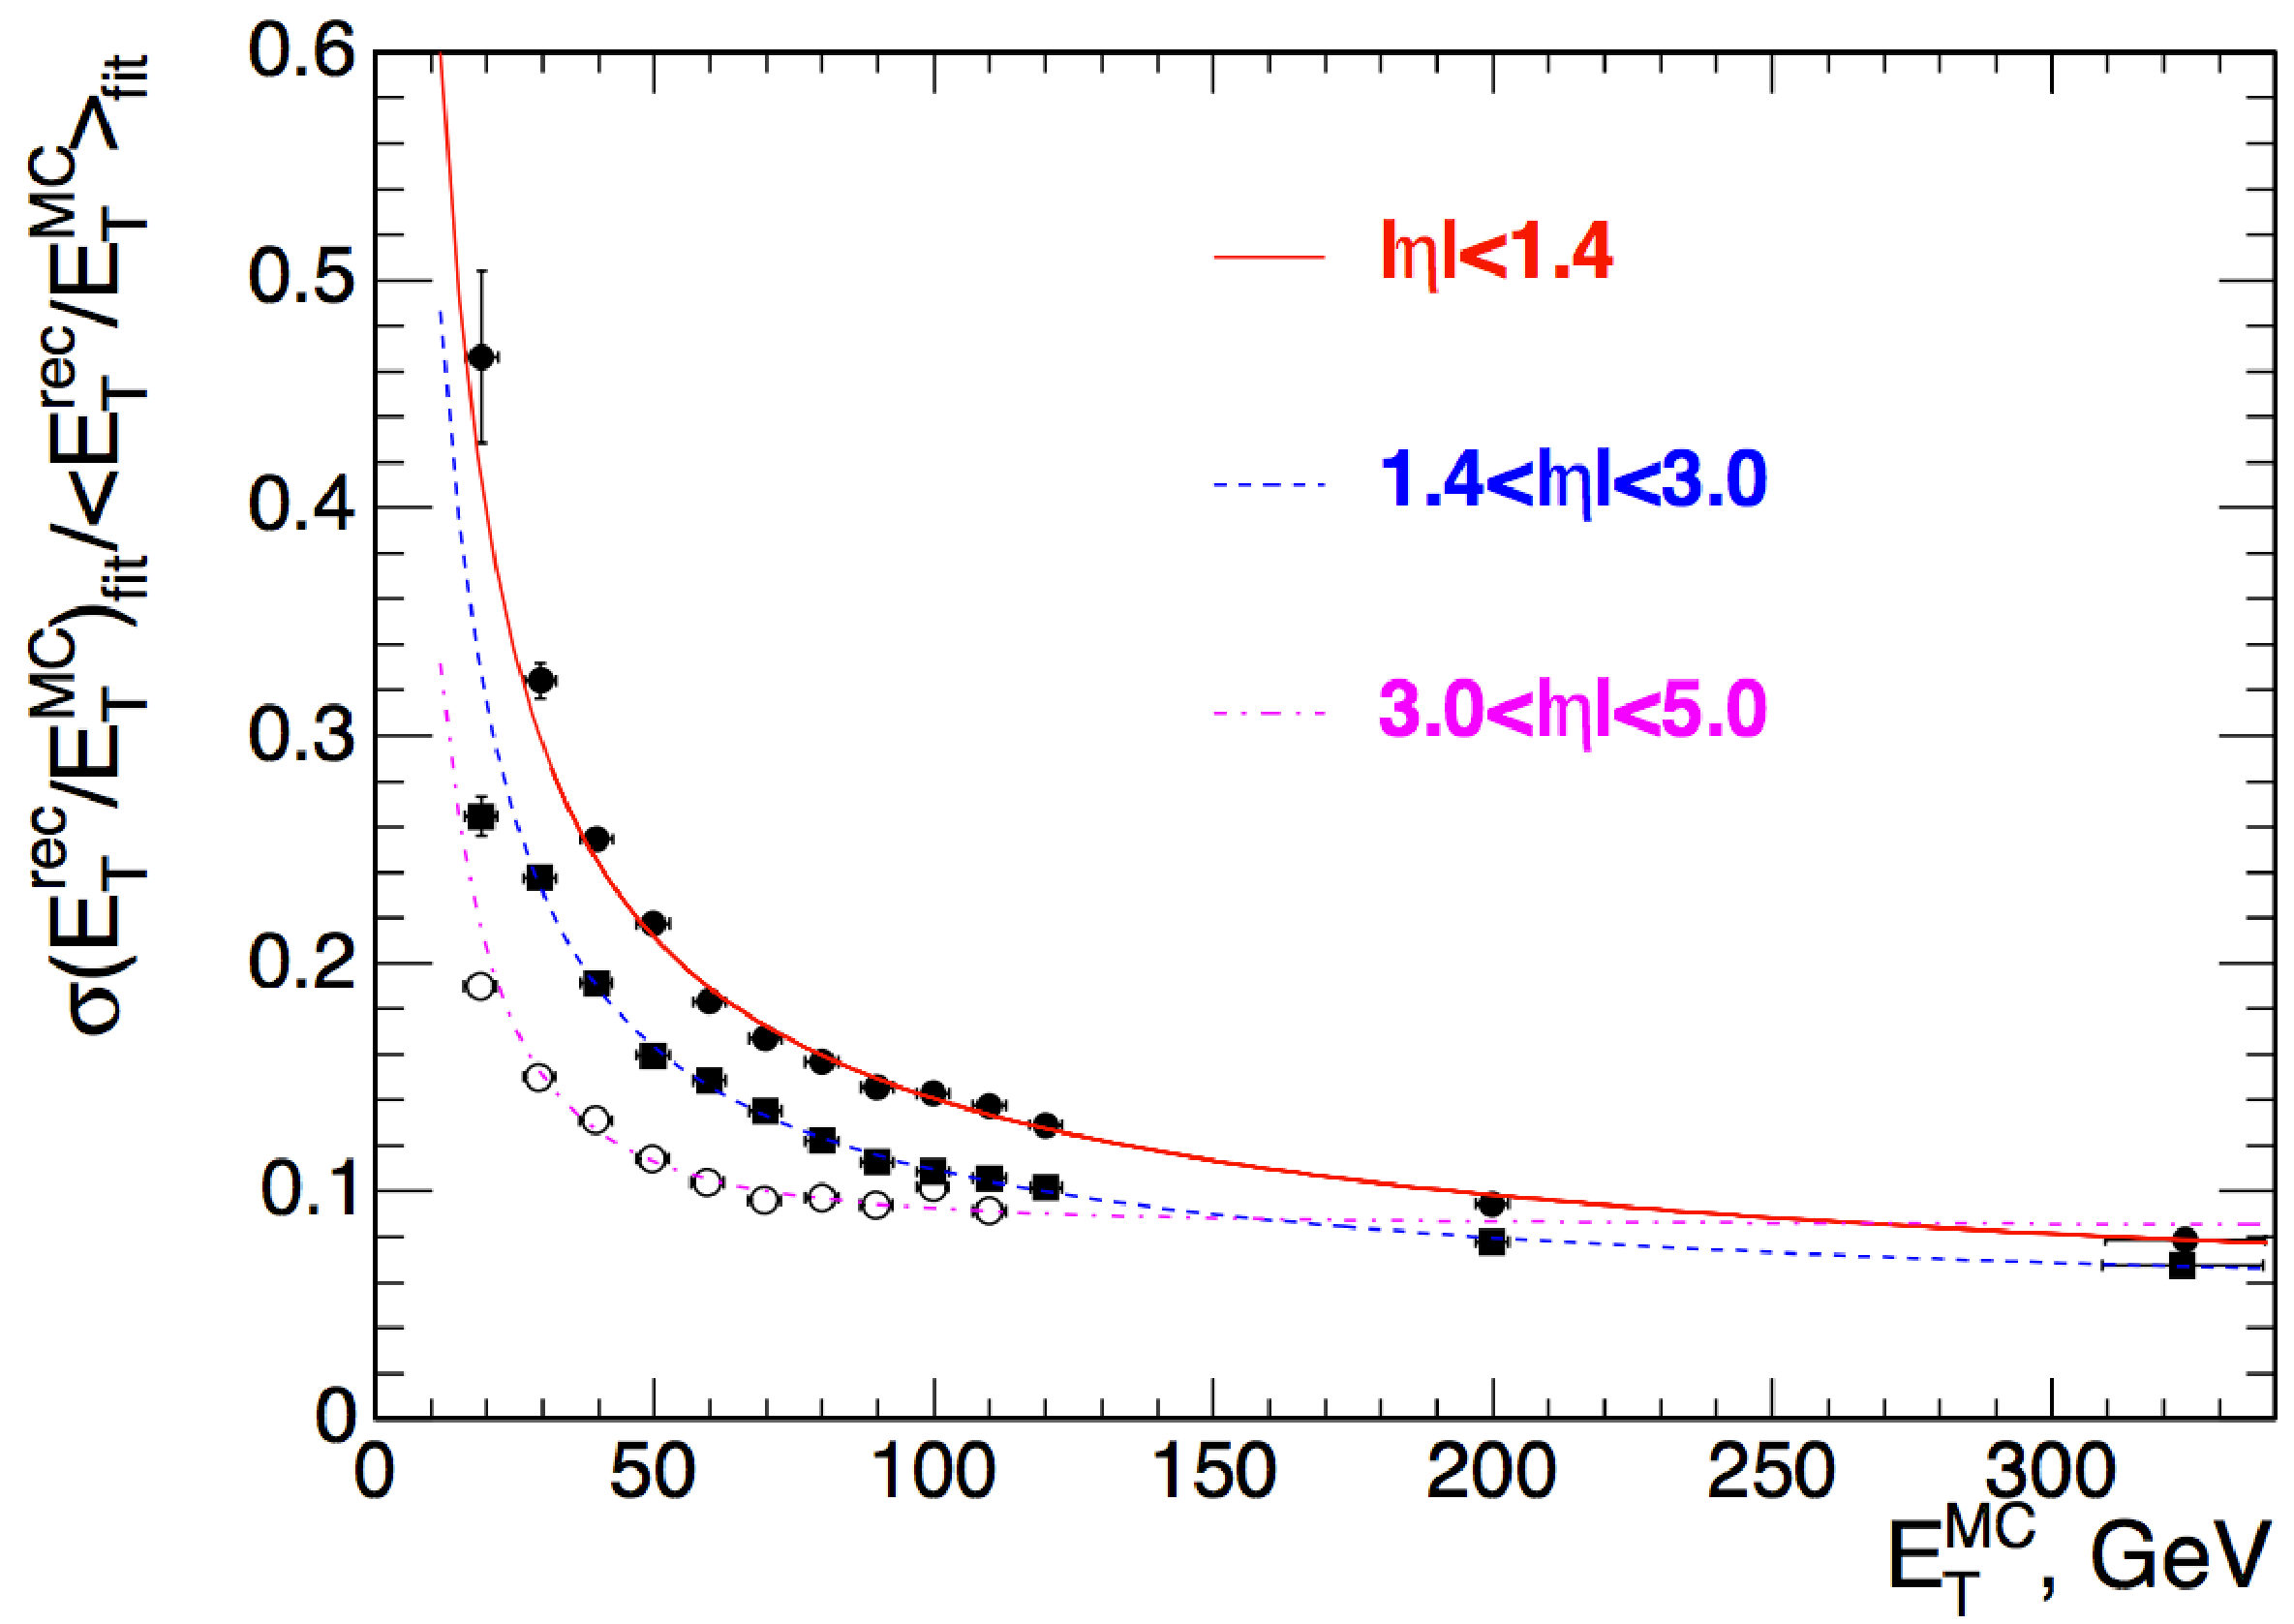
\includegraphics[width=.75\linewidth]{{LHC_CMS/HCALresolution}.pdf}
\caption[The jet transverse energy resolution as a function of the simulated jet transverse energy for barrel jets $\left(\abs{\eta} < 1.4\right)$, endcap jets $\left(1.4< \abs{\eta} <3.0\right)$ and very forward jets $\left(3.0< \abs{\eta} < 5.0\right)$]{The jet transverse energy resolution as a function of the simulated jet transverse energy for barrel jets $\left(\abs{\eta} < 1.4\right)$, endcap jets $\left(1.4< \abs{\eta} <3.0\right)$ and very forward jets $\left(3.0< \abs{\eta} < 5.0\right)$ \cite{Bayatian:922757}.}
\label{fig:HCALresolution}
\end{center}
\end{figure}

\subsection{Muon System}
\label{sec:Muon}

Muons at CMS are measured three times: in the inner tracker, after the magnet coil, and in the return flux. The muon system is designed to measure the path of the muons once they exit the magnet coil and as they traverse the return yoke. The momentum of the muons is measured by the bending angle of the muon's path as they exit the $\unit{4}{\tesla}$ coil taking the interaction point as the origin of the muon. The resolution at the origin of this measurement (hereafter referred to as ``muon system only") is dominated by multiple scatter in the material before the first muon station. This applies up to $p_{T} \sim \unit{200}{\GeVoverc}$, at which point the spatial resolution of the chamber states to dominate. For low-momentum muons, the best momentum resolution is determined by the silicon tracker (``inner tracker only"). However both systems contain information about the momentum and origin of muons, so CMS uses both of them (``full system") in concert to determine the momentum of muons produced in collisions. The momentum resolution can be seen in figure \ref{fig:MuonResolution}.

\begin{figure}
\begin{center}
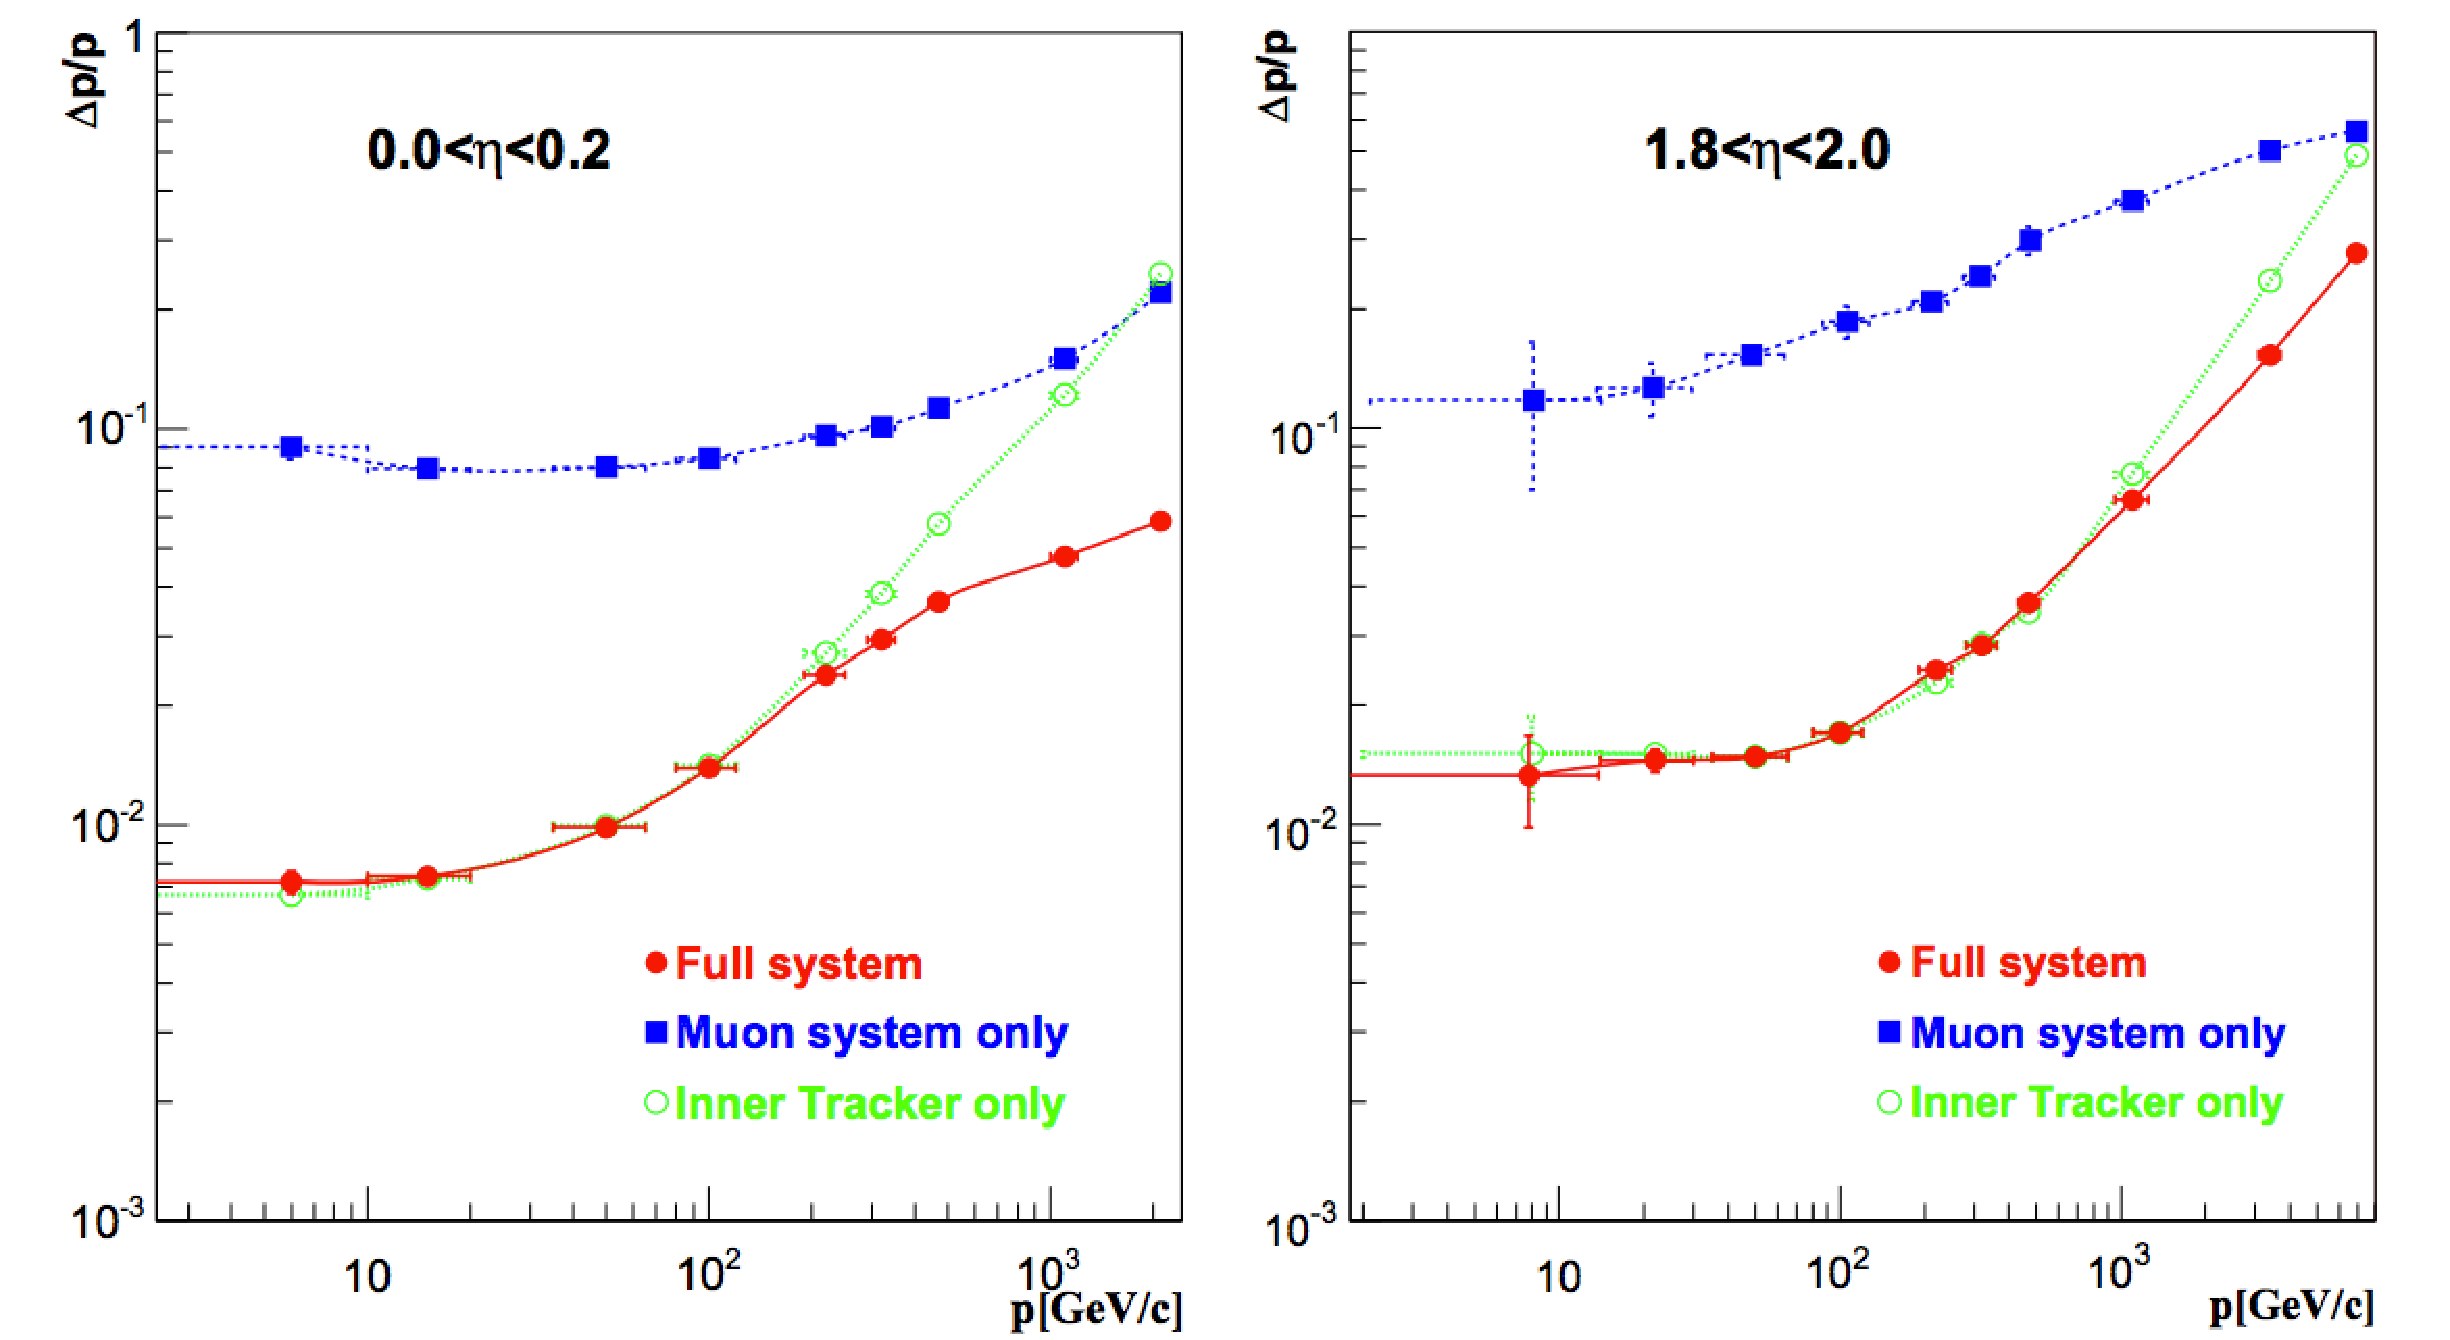
\includegraphics[width=0.75\linewidth]{{LHC_CMS/Muon_Resolution}.pdf}
\caption[The muon momentum resolution verses $p$ using the muon system only, the inner tracker only, or both (``full system"). (left) Barrel $\abs{\eta} < 0.2$ and (right) endcap $1.8 < \abs{\eta} < 2.0$.]{The muon momentum resolution verses $p$ using the muon system only, the inner tracker only, or both (``full system"). (left) Barrel $\abs{\eta} < 0.2$ and (right) endcap $1.8 < \abs{\eta} < 2.0$ \cite{Bayatian:922757}.}
\label{fig:MuonResolution}
\end{center}
\end{figure}

The muon system contains three types of gaseous detectors designed to cover the very large surface and the different radiation environments. The barrel region $\left( \abs{\eta} < 1.2 \right)$ is characterized by low neutron induced background, low muon rate, and low residual magnetic field in the chambers. For these reasons, drift tube (DT) chambers are used. In contrast the endcap region has high muon rates, neutron induced backgrounds, and residual magnetic field. So in the endcaps cathode strip chambers (CSC) are used to cover the region up to $\abs{\eta} < 2.4$. Both the endcap and barrel regions also use resistive plate chambers (RPC) which provide a fast response with good time resolution but lower position resolution than the DT and CSC systems. Taking the time information from the RPCs in concert with the position information from the CSCs and DTs provide necessary and complementary measurements. The whole system provides a precise and flexible detector that can be used for triggering and measurements.

The layout of one quarter of the CMS muon system is shown in figure \ref{fig:MuonDetectors}. In the barrel region, four stations of detectors are arranged in cylinders interlayered with the iron return yoke. The segmentation follows the five wheels of the yoke. In each of the endcaps, the CSC and RPC detectors are arranged with four disks perpendicular to the beam in concentric rings. In total, the muon system contains $\sim\unit{25000}{\squaremetre}$ of active detection planes with $\sim 1$ million electronic channels.

\begin{figure}
\begin{center}
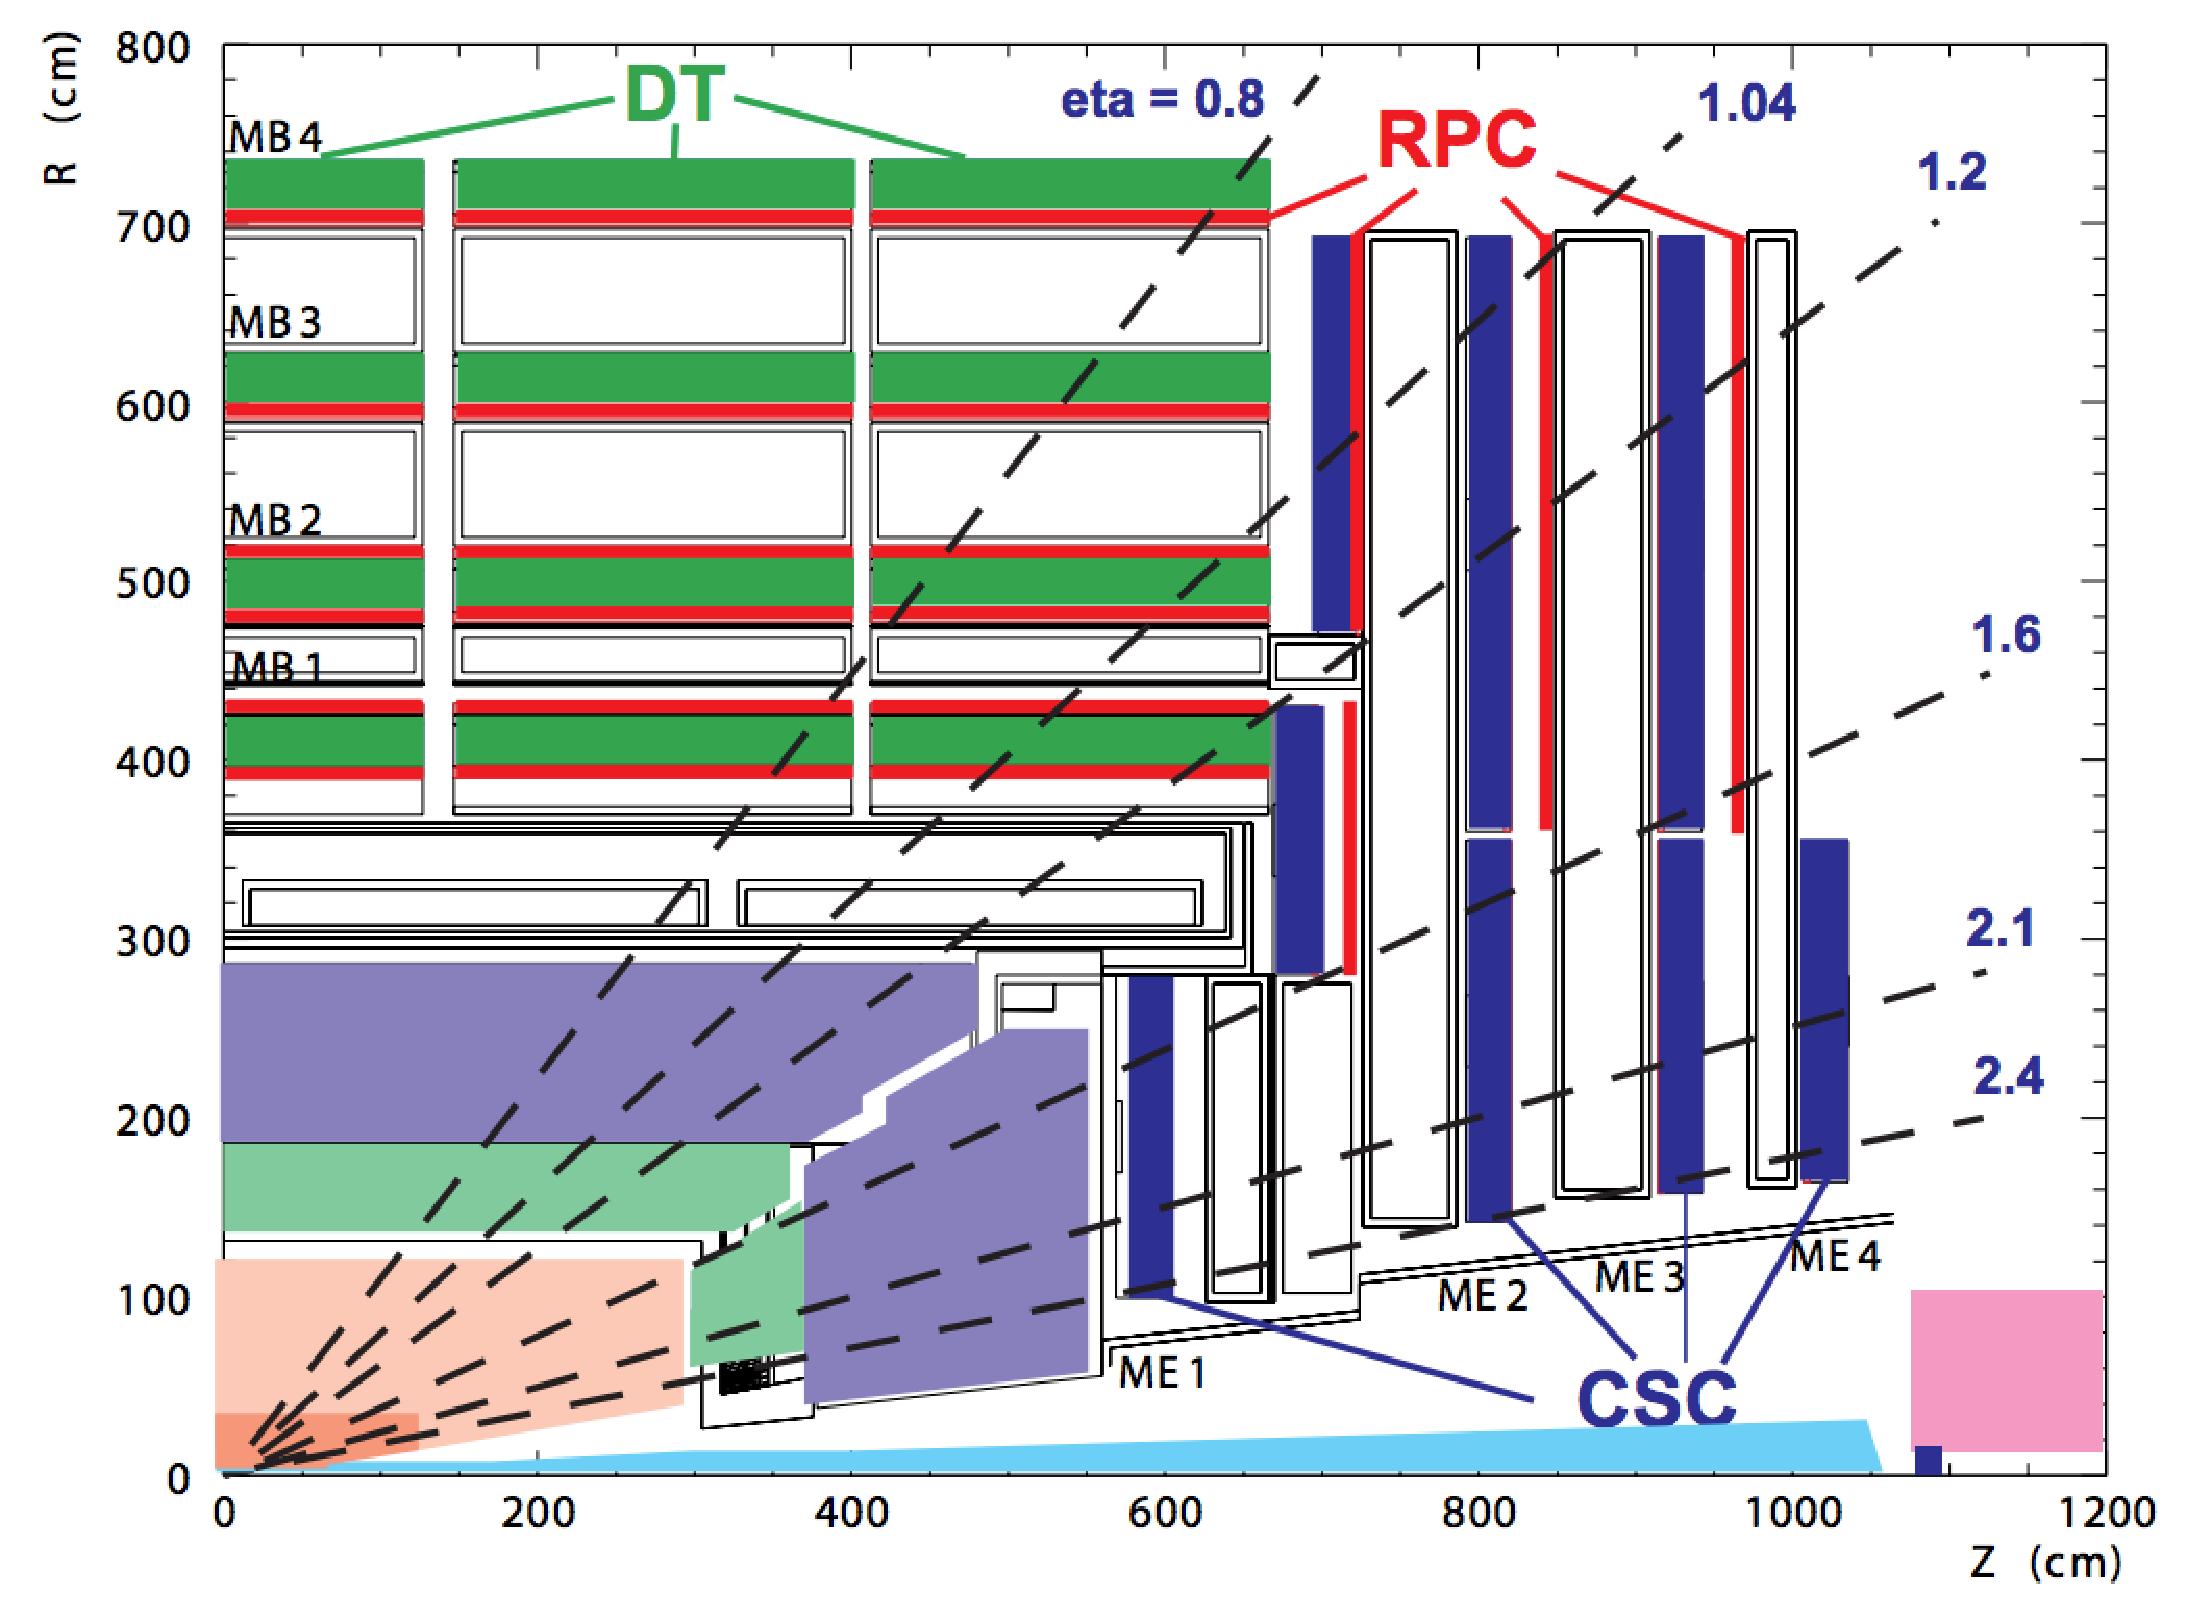
\includegraphics[width=0.75\linewidth]{{LHC_CMS/Muon_Detectors}.pdf}
\caption[Layout of one quarter of the CMS muon system for initial low luminosity running. The RPC system is limited to $\abs{\eta} < 1.6$ in the endcap, and for the CSC system only the inner ring of the ME4 chambers have been deployed]{Layout of one quarter of the CMS muon system for initial low luminosity running. The RPC system is limited to $\abs{\eta} < 1.6$ in the endcap, and for the CSC system only the inner ring of the ME4 chambers have been deployed\cite{Bayatian:922757}.}
\label{fig:MuonDetectors}
\end{center}
\end{figure}

The barrel detectors consist of 250 chambers organized in four layers inside the magnet return yoke, at radii of approximately $\unit{4.0, 4.9, 5.9, 7.0}{\meter}$ from the beam axis. Each DT chamber in the three innermost stations consists of 12 layers of drift tubes divided into three groups of four consecutive layers, hereafter called SuperLayers (SL). The tubes inside each SL are staggered by half a tube. Two SLs measure the $r-\phi$ coordinate in the bending plane (they have wires parallel to the beam line), and the third SL measures the $z$-coordinate running parallel to the beam.  In the outermost station each DT chamber has only the two SLs that measure the $r-\phi$ coordinate. The two innermost stations consist of �sandwiches� made of a DT chamber placed between 2 RPCs. The two outermost stations consist of packages of a DT chamber coupled to a layer made of 1, 2, or 4 RPCs, depending on the sector and station, placed on the innermost side of the station. The maximum drift length in the barrel is $\unit{2.0}{\centi\meter}$ and the single-point resolution is $\sim \unit{200}{\micro\meter}$, giving a $\phi$ precision better than $\unit{100}{\micro\meter}$ in position and approximately $\unit{1}{\milli\rad}$ in direction.

In the two endcaps, 468 CSCs arranged in four stations of chambers which are mounted in disks enclosing the CMS magnet, perpendicular to the beam direction. Each CSC is a trapezoidal in shape and consists of six gas gaps, each gap having a plane of radial cathode strips and plane of anode wires running almost perpendicularly to the strips. Most CSCs are overlapped in $\phi$ to avoid gaps in the muon acceptance\footnote{The exception being the third ring of the first endcap disk.}. Each ring station consists of 36 chambers, except for the innermost ring of the second, third, and fourth disks which have 18 chambers. A precise position measurement is made by determining the center-of-gravity of the charge distribution induced on the cathode strips with a spatial resolution $\sim\unit{200}{\micro\meter}$ and angular resolution in $\phi \sim \unit{10}{\milli\rad}$. Like in the Barrel, there are layers of double-gap RPCs in the endcaps, however, for the initial low-luminosity run there are RPCs only in the outer rings of each station, while they are staged in the internal rings. The RPC endcap system is thus limited to $\eta < 1.6$ for the first period of data taking.

\section{Triggering and Particle Reconstruction}
\label{sec:TriggerANDreconstruction}

At the designed specifications the LHC would lead to $\sim 10^{9}$ interactions/sec. Data from only about $10^{2}$ crossings/sec can be written to archival media; hence, the trigger system has to achieve a rejection factor $10^{6}$. This is performed by the CMS trigger and data acquisition system which consists of four parts: the detector electronics, the Level-1 trigger, the readout network, and an online event filter system (processor farm) that executes the software for the High-Level Triggers (HLT).

Once the data is archived, CMS must analyze this data and reconstruct the individual particles that make up the event. A particle flow event-reconstruction algorithm (PF) has been successfully deployed in the CMS experiment and is nowadays used by most of the analyses. It aims at identifying and reconstructing individually each particle arising from the LHC proton-proton collision, by combining the information from all the subdetectors. Using this algorithm individual particles can be identified as photons, electrons, muons, or charged/neutral hadrons.

\subsection{CMS Trigger}

The size of the LHC detectors and the underground caverns that they reside in imposes a minimum transit time for the signals from the front-end electronics to reach the services cavern which houses the Level-1 trigger logic. A signal must pass from the various subdetectors we have discussed to this Level-1 system and back again to signal a readout of the full detector. The total time allocated for the transit and for reaching a decision to keep or discard data from a particular beam crossing is $\unit{3.2}{\micro\second}$. During this time, the detector data is held in buffers while trigger data is collected form the front-end electronics and decisions reached that discard a large fraction of events while regaining the small fraction of interactions of interest (approx. 1 in 1000). Of the total latency, the time allocated to the Level-1 trigger calculations is less than $\unit{1}{\micro\second}$.

Custom hardware processors form the Level-1 decision. The Level-1 triggers involve the calorimetry and muons systems, as well as some correlation of the information between these systems. These Level-1 decisions are based on the presence of ``trigger primitive" objects such as photons, electrons, muons, and jets above a set of $E_{T}$ and $p_{T}$ thresholds that have reduced granularity and resolution. It also employs global sums of $E_{T}$ and $E_{T}^{\text{miss}}$. The designed Level-1 pass rate is $\unit{100}{\kilo\hertz}$, but was limited to $\unit{50}{\kilo\hertz}$ at startup.

Upon receipt of a Level-1 trigger, the data from the pipelines are transferred to front-end readout buffers. After further signal processing, zero-suppression and/or data-compression each event will have a size of about $\unit{1.5}{\mega\text{B}}$ for proton-proton interactions. Data from a given event are then transferred to a processor that runs the high-level trigger (HLT) software to reduce the Level-1 output rate of $\unit{100}{\kilo\hertz}$ down to $\unit{100}{\hertz}$ for mass storage. Rather than reconstruct all possible objects in an event for HLT, whenever possible only those objects and regions of the detector that are actually needed for the decision are reconstructed. In that way events are discarded as soon as possible, events that still pass are then stored across the ``LHC Computing Grid"\footnote{Specifics of this vast and complex GRID computing network are not discussed here.} for later software analysis by individuals searching for specific physics phenomenon.

\subsection{Particle Flow}

The particle-flow event reconstruction aims at reconstructing and identifying all stable particles in the event, i.e., electrons, muons, photons, charged hadrons and neutral hadrons, with a thorough combination of all CMS sub-detectors towards an optimal determination of their direction, energy and type. This list of individual particles is then used to build jets (from which the quark and gluon energies and directions are inferred), to determine the missing transverse energy $E_{T}^{\text{miss}}$ (which gives an estimate of the direction and energy of the neutrinos and other invisible particles), to reconstruct and identify taus, $\tau$, from their decay products, to quantify charged lepton isolation with respect to other particles, to tag $b$ jets, etc \cite{CMS-PAS-PFT-09-001}.

While this algorithm is extremely versatile we will focus our discussion on the pieces that are relevant for this analysis: electrons, muons, and jets. A small discussion will also be made of photons which are used in this analysis as well. 

\subsection{Electrons}

The electron reconstruction combines ECAL and tracker information. Electron candidates are reconstructed from clusters of energy deposits in the ECAL, which are then matched to hits in the silicon tracker and silicon tracker seeds that are mapped to ECAL clusters. This dual approach improves the reconstruction efficiency for the very low $p_{T}$ electrons. The CMS electron reconstruction algorithm is described in \cite{CMS-PAS-EGM-10-004,Chatrchyan:2013mxa}. 

For this physics analysis, the electron candidates are required to have transverse momentum $p^{e}_{T} > \unit{7}{\GeVoverc}$ and a reconstructed $\abs{\eta} < 2.5$. The reconstruction efficiency for isolated electron is expected to be above 90\% over the full ECAL acceptance, apart from some narrow ``crack" regions. 

The identification of electrons relies on a Boosted Decision Tree (BDT) multivariate technique that combines observables sensitive to the amount of bremsstrahlung along the electron trajectory, the geometrical and momentum matching between the electron trajectory and associated clusters, as well as shower-shape observables. The distribution of expected and observed electron BDT output is shown in figure \ref{fig:Ele_BDT}. The selection is optimized in six regions of the electron $p^{e}_{T}$ and $\abs{\eta^{e}}$ to maximize
the expected sensitivity for a low-mass Higgs boson. These regions correspond to two $p^{e}_{T}$ ranges, $\unit{7--10}{\GeV}$ and $>\unit{10}{\GeV}$, and three pseudorapidity regions, corresponding to two regions in the barrel with different material in front of the ECAL, the central barrel $\left(\abs{\eta^{e}} < 0.8\right)$ and the outer barrel $\left(0.800 < \abs{\eta^{e}} < 1.479\right)$, in addition to the endcap, $1.479 < \abs{\eta^{e}} < 2.500$.

\begin{figure}
\begin{center}
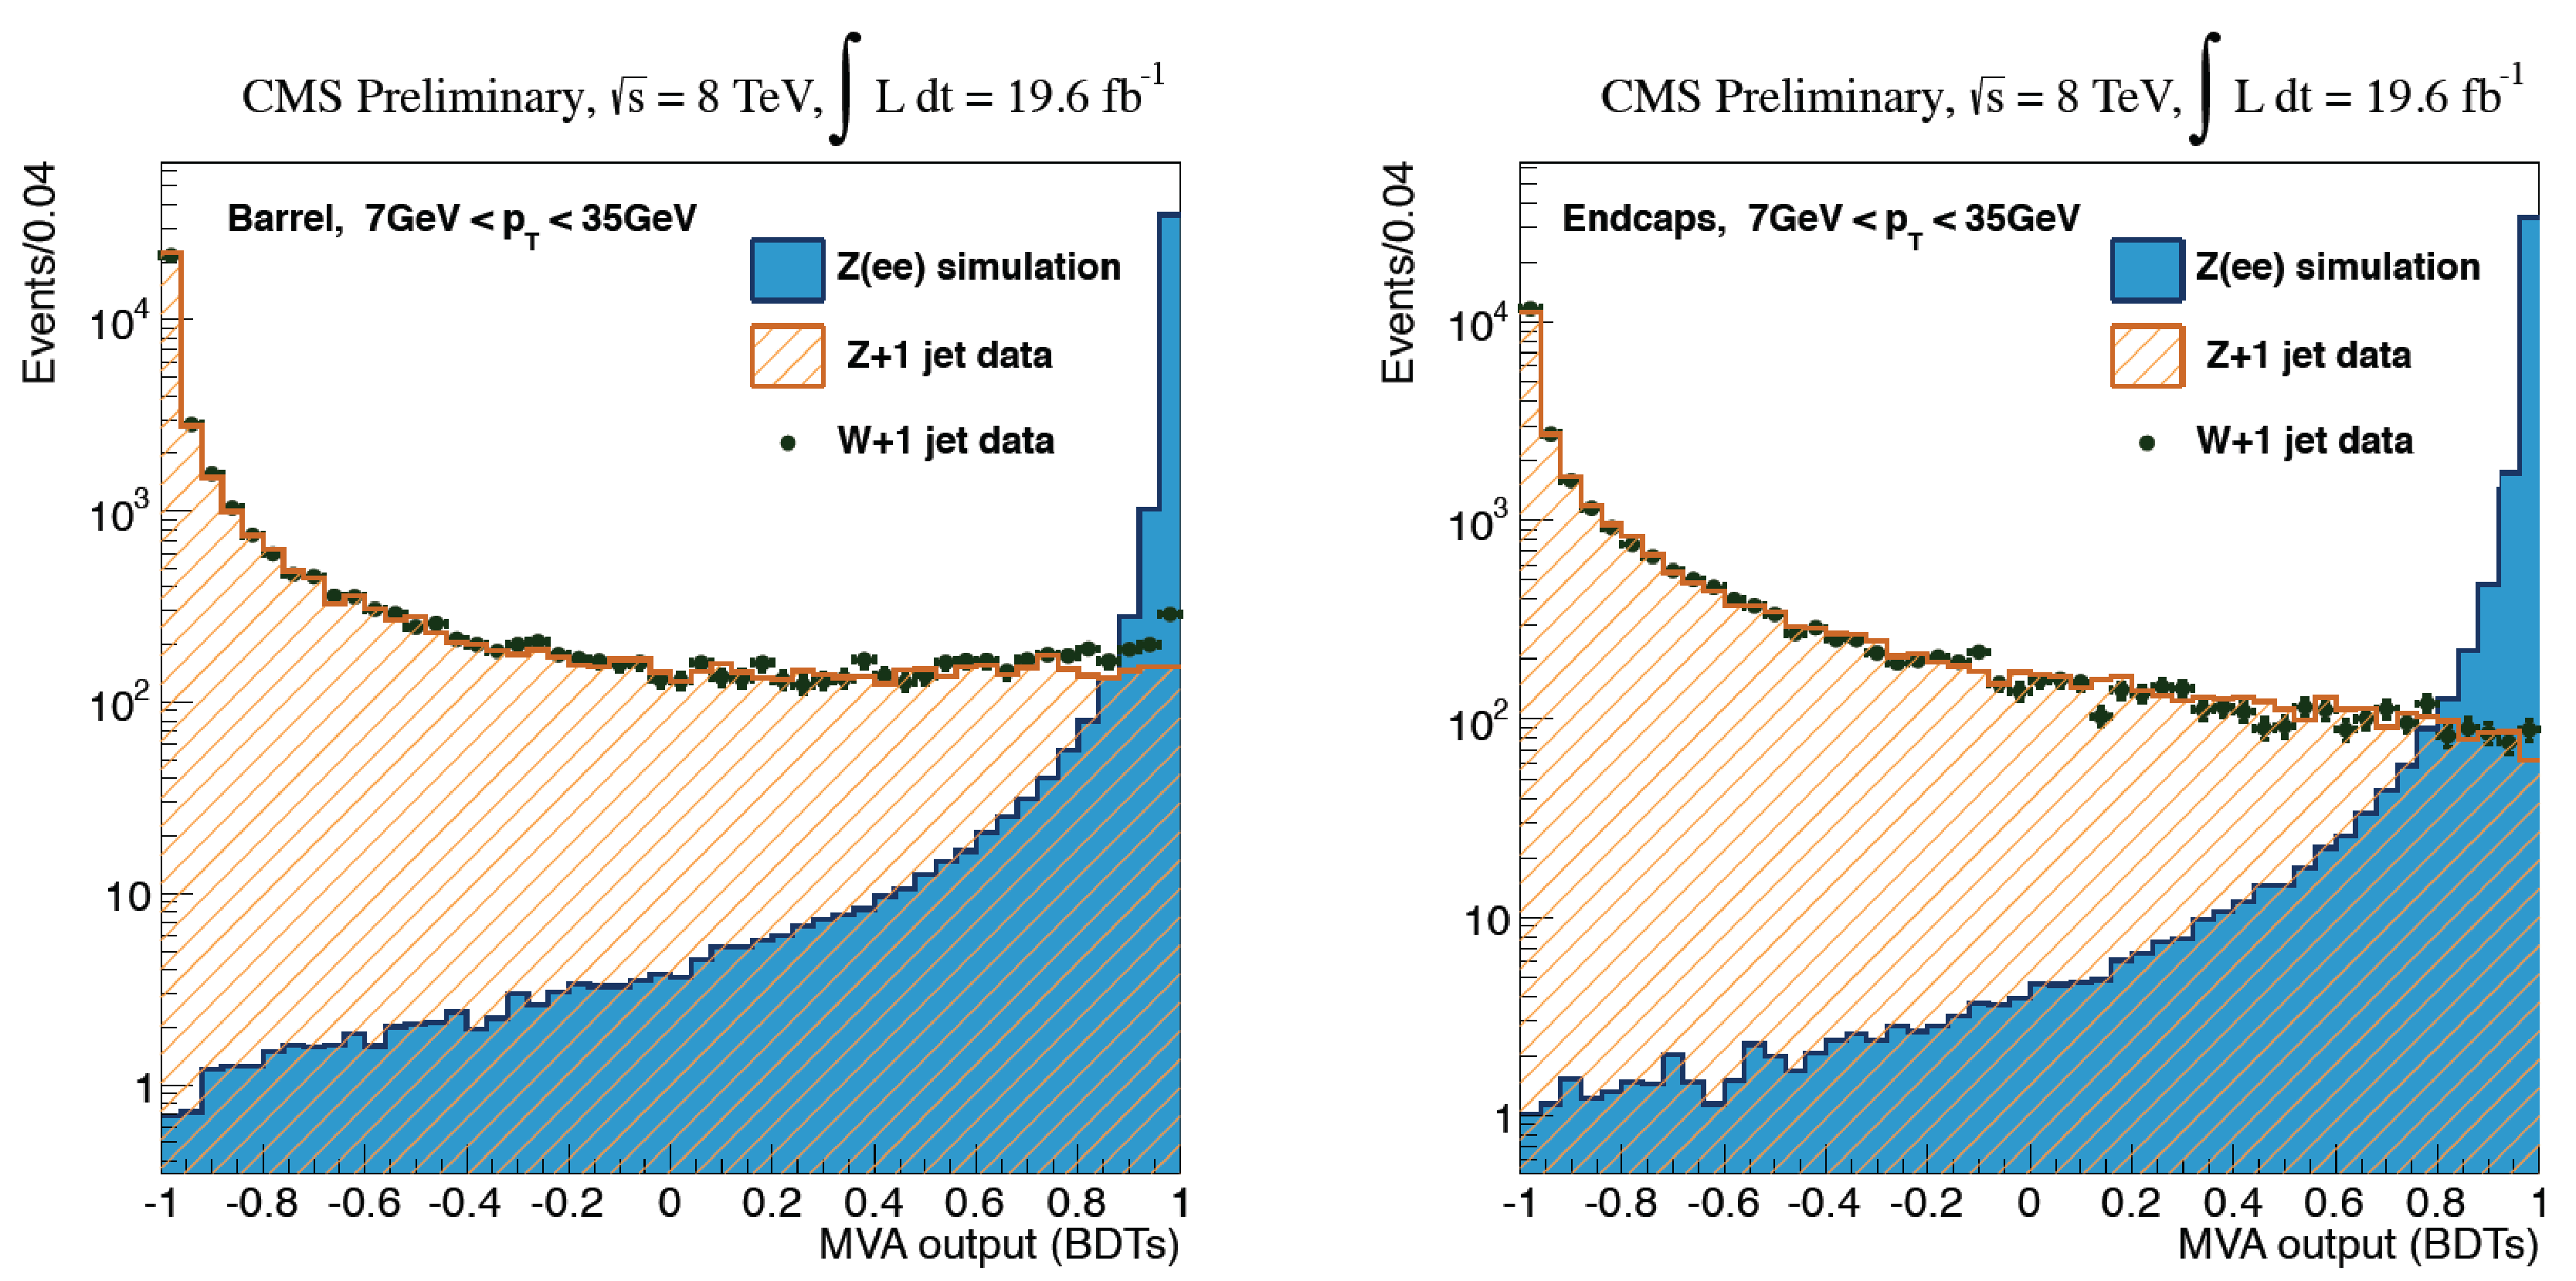
\includegraphics[width=0.75\linewidth]{{LHC_CMS/Ele_BDT}.pdf}
\caption[Distribution of electron BDT output for training sample $W+$jets, test sample $Z+$jets on 2012 data (fakes) and prompt electrons ($Z \to ee$ simulation) in the barrel (left) and endcap(right)]{Distribution of electron BDT output for training sample $W+$jets, test sample $Z+$jets on 2012 data (fakes) and prompt electrons ($Z \to ee$ simulation) in the barrel (left) and endcap(right)\cite{CMS-DP-2013-003}.}
\label{fig:Ele_BDT}
\end{center}
\end{figure}

The quality of the momentum measurement for electrons can substantially vary depending on the electron characteristics. The resolution is mainly dominated by the fluctuations of the measured energy due to bremsstrahlung in the tracker material. This entails that the $4\ell$ mass resolution varies broadly, by as much as a factor of 2-3. Therefore, mixing together events with well and poorly measured $4\ell$ masses dilutes the Higgs boson search sensitivity, and mass measurement. The analysis uses the propagation of the lepton uncertainty to estimate the $4\ell$ mass to proper accounting for the signal mass resolutions for individual events. In order to have a good determination of this uncertainty, but above all to have a description of the resolution of the signal model which corresponds to the data, we need to measure it on high statistics control samples, depending on the electron kinematics and quality, which is done with $Z \to ee$ sample. The absolute scale has also to be calibrated on data, because the measurement of the Higgs boson mass depends crucially on the uncertainty that we can assign to the leptons in the full phase space of the analysis for a $\unit{125}{\GeV}$ Higgs boson, so covering from $\unit{7--100}{\GeV}$, which can be covered with $Z \to ee$ and low mass resonances.

For electrons, the calibration procedure consists of three steps. First, a set of corrections for the momentum scale is obtained by comparing the displacement of the peak position in the distributions of the Z-boson mass in the data and in the simulation in different $\eta$ regions and in two categories depending on the amount of bremsstrahlung. The corrections are derived as a function of time in order to account for the time-dependent crystal transparency loss. Second, a linearity correction to the momentum scale is applied to account for the $p_{T}$-dependent differences between data and simulation by comparing the dielectron mass distributions, binned in $p^{e}_{T}$ of one of the two electrons, in data and in simulated $Z \to ee$ events. The $J/\psi \to ee$ and $\Upsilon\left(1S\right) \to ee$ events are used as validation for electron $p^{e}_{T} < \unit{20}{\GeV}$. All the corrections on the electron momentum scale from the first two steps are applied to data. The left of figure \ref{fig:Ele_scale_res} shows the residual momentum scale difference before the linearity correction but after the time dependent corrections. Third, the energies of single electrons in the simulation are smeared by applying a random Gaussian multiplicative factor of mean 1 and width $\Delta\sigma$, in order to achieve the resolution observed in the data Z-boson sample. The result of this resolution correction is shown on the right of figure \ref{fig:Ele_scale_res}.

After the electron calibration, the relative momentum scale between data and simulation is consistent within 0.6\% in the central barrel and up to $\sim 1.5\%$ in the forward part of the ECAL endcaps. The residual dependence at low momentum is due to the use of wide bins in measured electron $p^{e}_{T}$ in evaluating the Z-peak mass shift. The resulting shift of 0.3\% (0.1\%) for the $4e \left(2e2\mu\right)$ channel is assigned as a systematic uncertainty in the signal mass scale.

\begin{figure}
\begin{center}
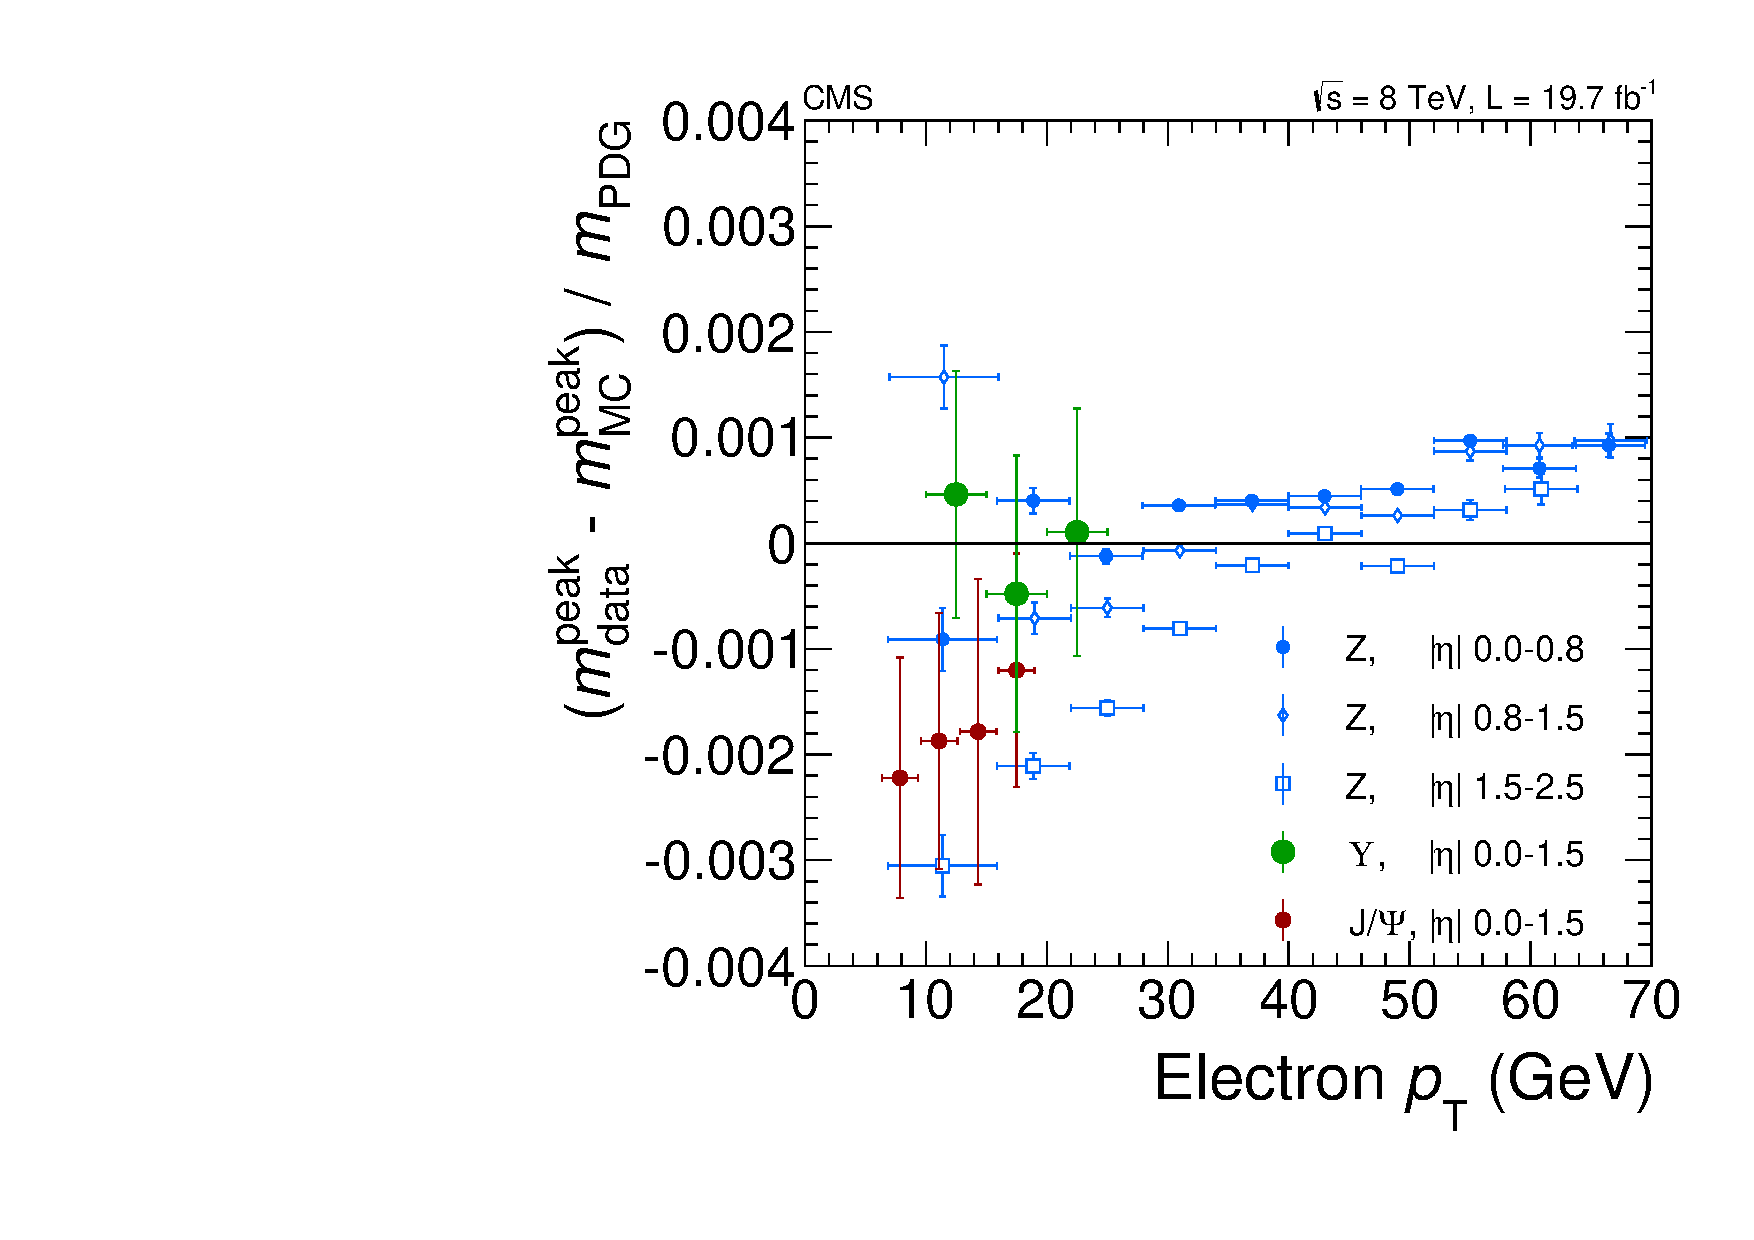
\includegraphics[width=0.45\linewidth]{{LHC_CMS/scale-ptdep-8TeV}.pdf}
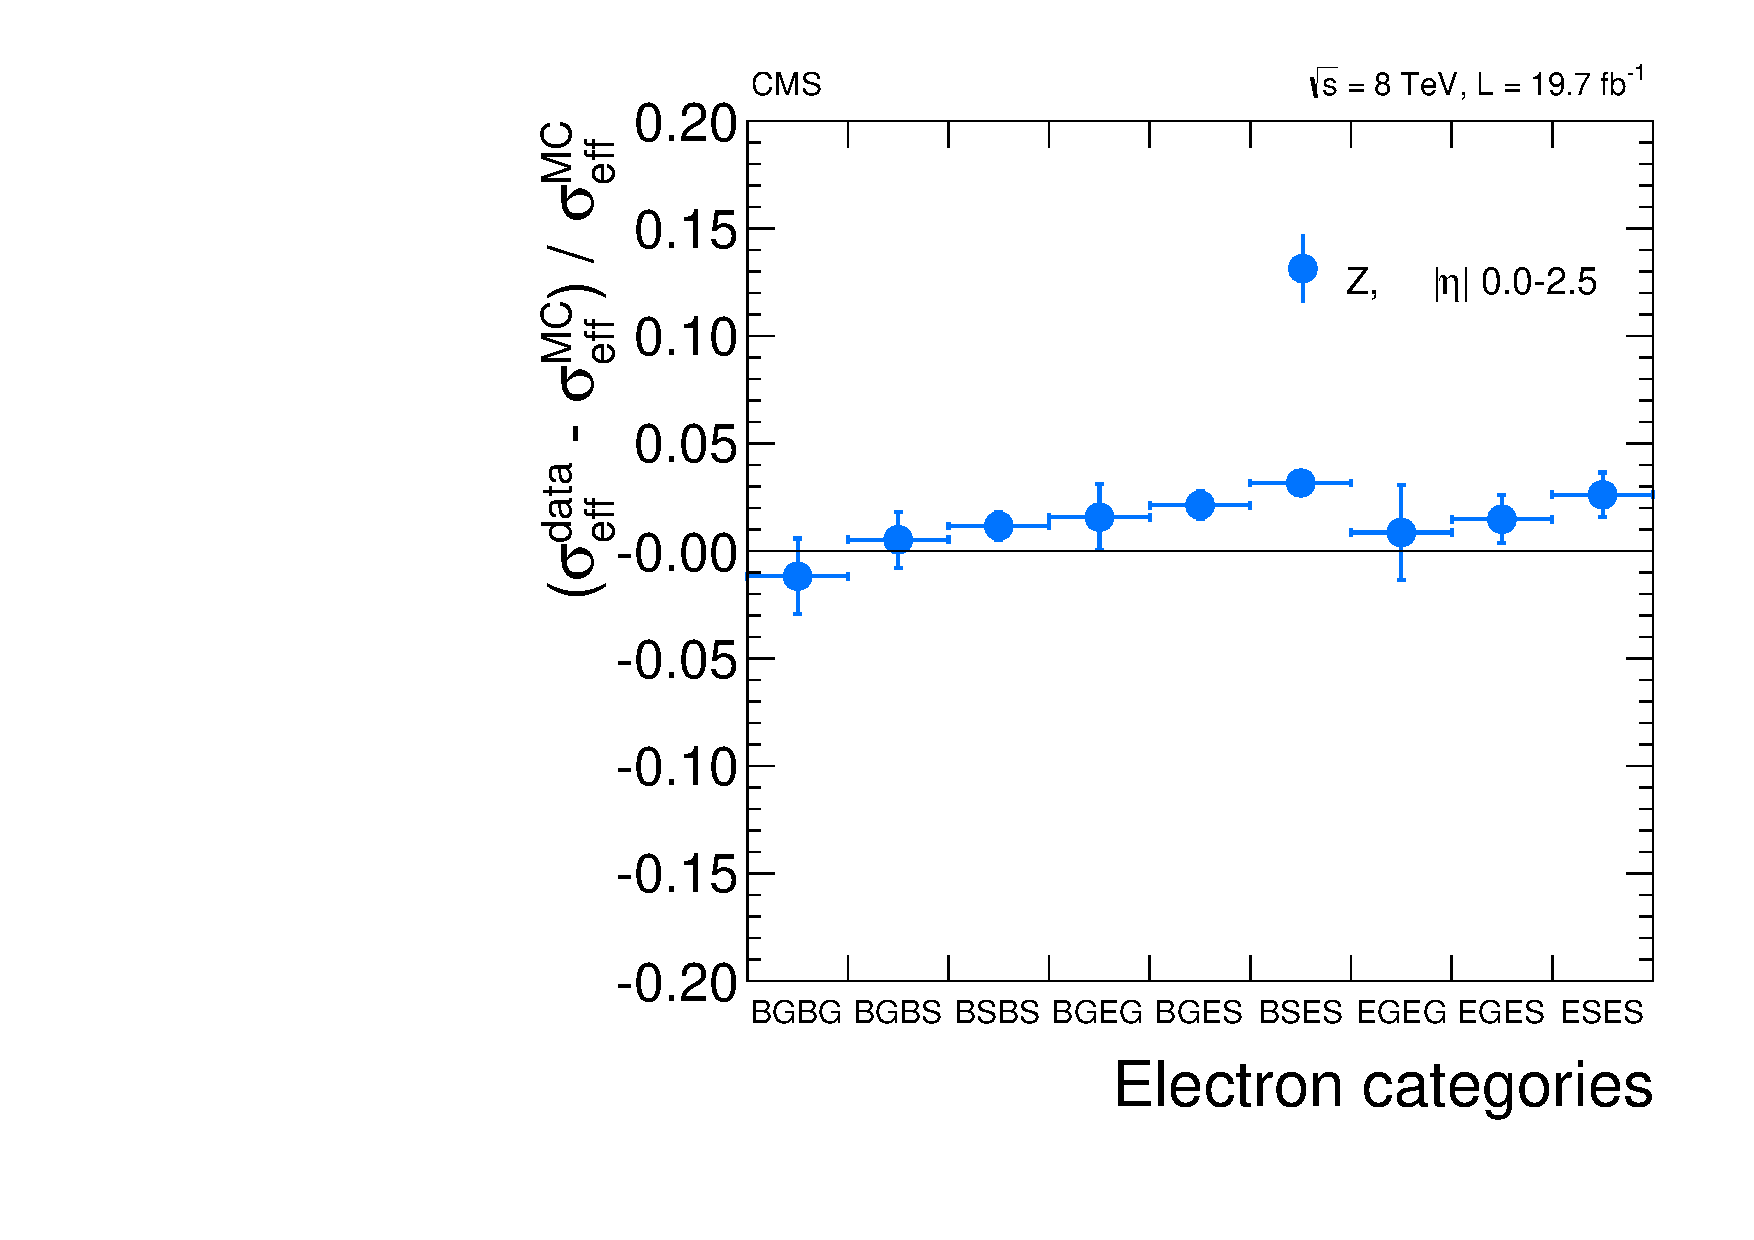
\includegraphics[width=0.45\linewidth]{{LHC_CMS/electron_resolution}.pdf}
\caption[(left) Relative difference between the dilepton mass peak positions in data and simulation as obtained from Z, $J/\psi$ and $\Upsilon\left(nS\right)$ resonances as a function of the transverse momentum of one of the electrons regardless of the second for dielectron events before $p_{T}$ dependent correction. (right) Relative difference between the dilepton mass peak positions in data and simulation as obtained from Z, $J/\psi$ and $\Upsilon\left(nS\right)$ resonances as a function of the transverse momentum of one of the electrons regardless of the second for dielectron events.]{(left) Relative difference between the dilepton mass peak positions in data and simulation as obtained from Z, $J/\psi$ and $\Upsilon\left(nS\right)$ resonances as a function of the transverse momentum of one of the electrons regardless of the second for dielectron events before $p_{T}$ dependent correction. (right) Relative difference between the dilepton mass peak positions in data and simulation as obtained from Z, $J/\psi$ and $\Upsilon\left(nS\right)$ resonances as a function of the transverse momentum of one of the electrons regardless of the second for dielectron events\cite{Chatrchyan:2013mxa}.}
\label{fig:Ele_scale_res}
\end{center}
\end{figure}

\subsection{Muons}
\label{sec:Muons}

Muon candidates are required to have a transverse momentum $p^{\mu}_{T} > \unit{5}{\GeV}$ and be within the geometrical acceptance, defined by $\abs{\eta^{\mu}} < 2.4$. The reconstruction combines information from both the silicon tracker and the muon system. The matching between track segments is done either outside-in, starting from a track in the muon system, or inside-out, starting from a track in the silicon tracker. The muons are selected among the reconstructed muon track candidates by applying minimal requirements on the track segments in both the muon system and inner tracker system and taking into account compatibility with small energy deposits in the calorimeters\cite{Chatrchyan:2013mxa}.

For muons, an absolute measurement of momentum scale and resolution is performed by using a reference model of the Z line shape convolved with a Gaussian function. The bias in the reconstructed muon $p_{T}$ is determined from the position of the Z mass peak as a function of muon kinematic variables, and a correction is derived for the data. A correction for the resolution is also derived for the simulation from a fit to the $Z \to \mu\mu$ mass spectrum. The large event sample based on low-mass dimuon resonances provides an additional calibration source for the momentum resolution in a similar manner. For muons, the agreement between the observed and simulated mass scales is within 0.1\% in the entire pseudorapidity range of interest and assigned as a systematic.

\begin{figure}
\begin{center}
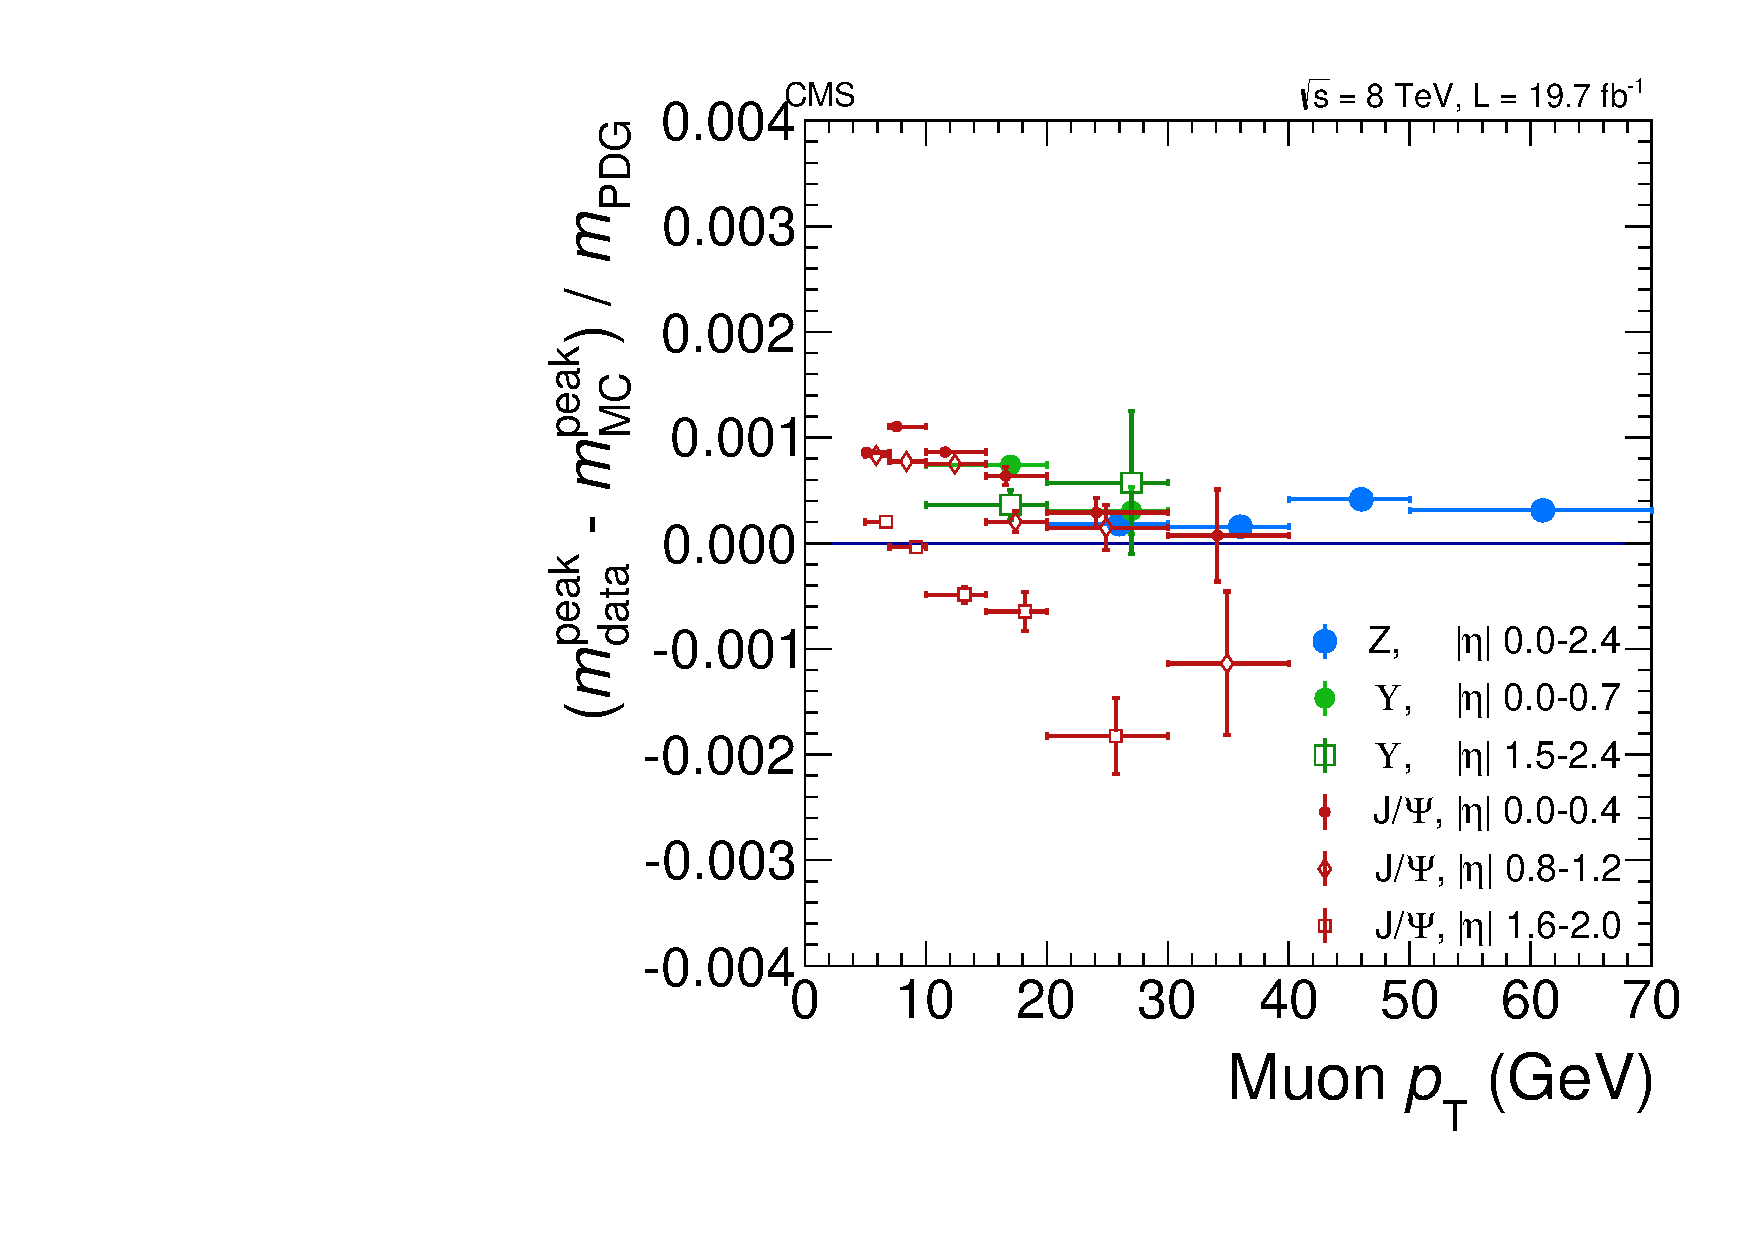
\includegraphics[width=0.45\linewidth]{{LHC_CMS/100_scale_mf}.pdf}
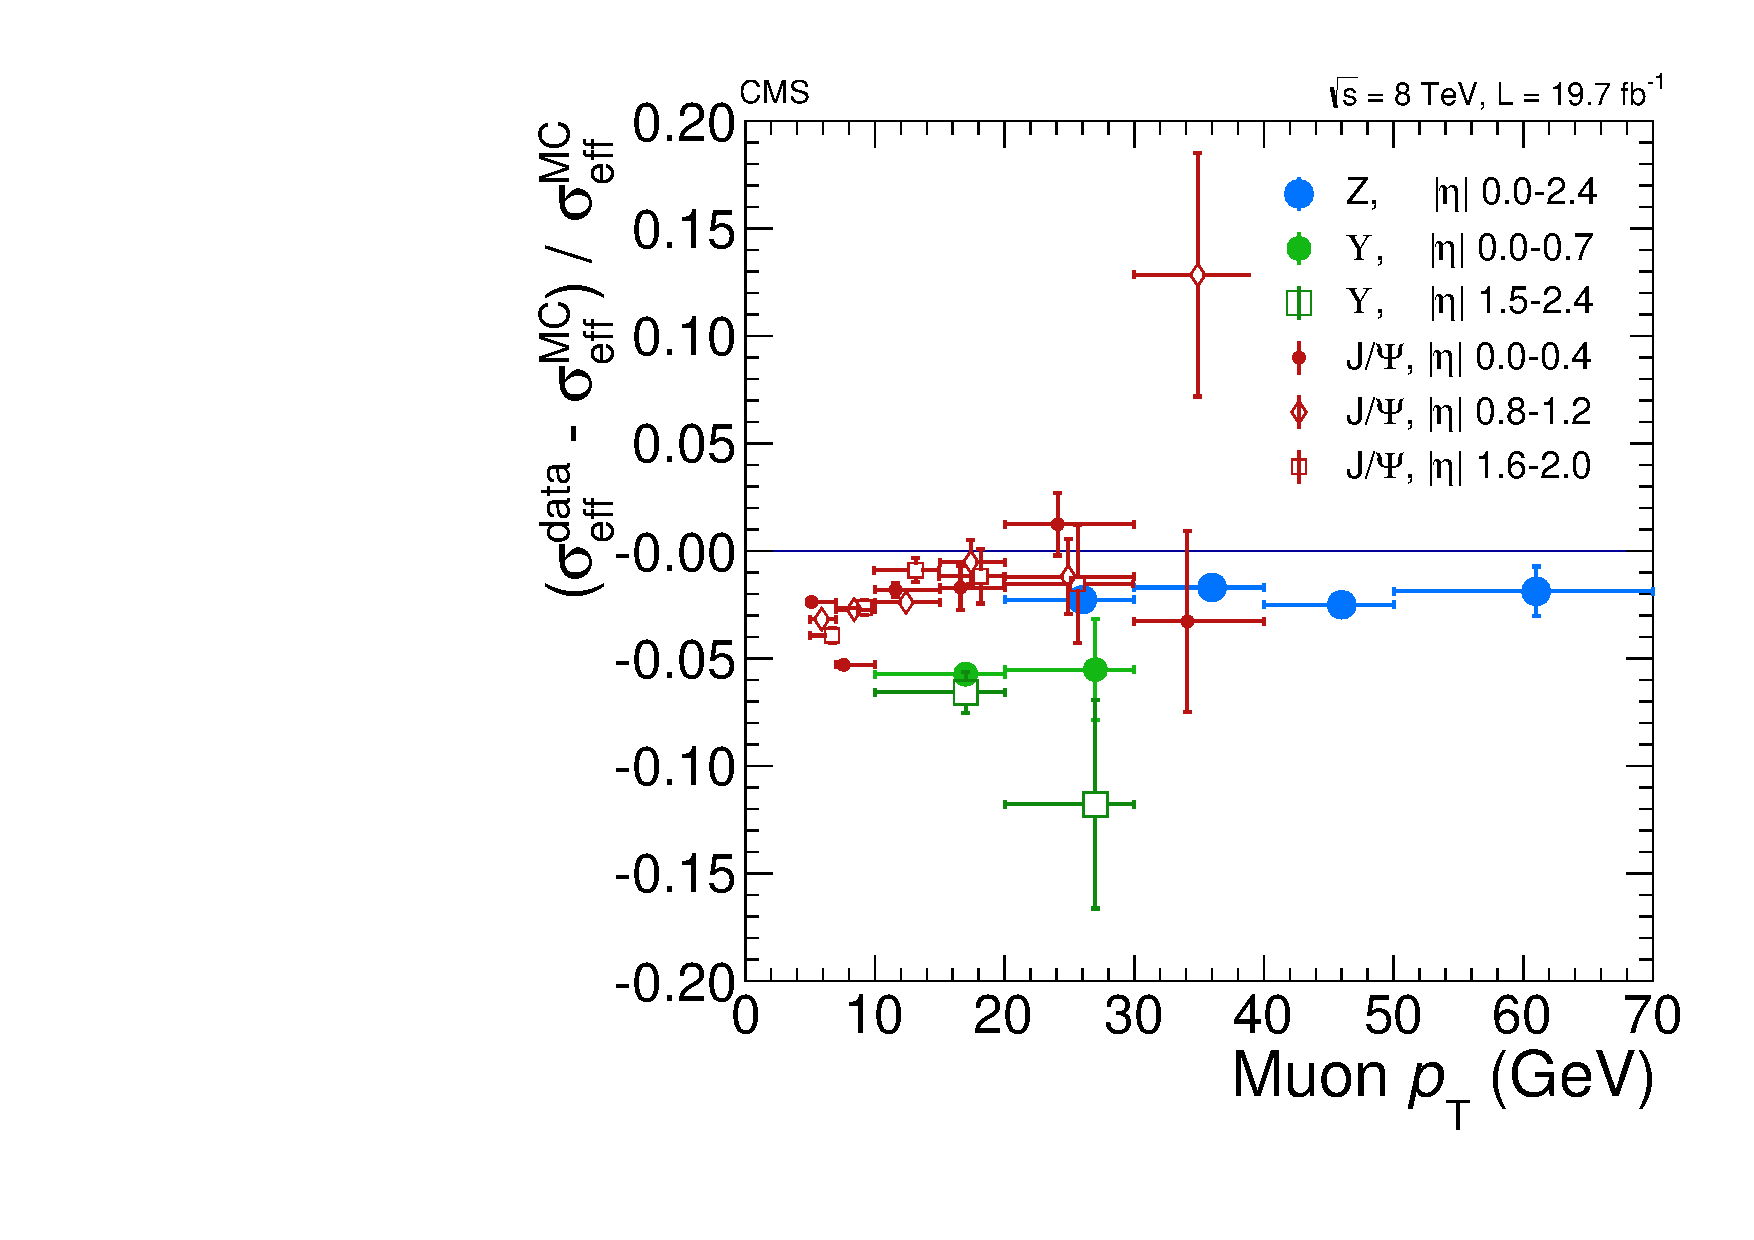
\includegraphics[width=0.45\linewidth]{{LHC_CMS/100_resolution_mf}.pdf}
\caption[(left) Relative difference between the dilepton mass peak positions in data and simulation as obtained from Z, $J/\psi$ and $\Upsilon\left(nS\right)$ resonances as a function of the average muon $p^{\mu}_{T}$ for dimuon events. (right) Relative difference between the dimuon mass resolutions in data and simulation as measured fromZ, $J/\psi$ and $\Upsilon\left(nS\right)$ decays as functions of the average muon]{(left) Relative difference between the dilepton mass peak positions in data and simulation as obtained from Z, $J/\psi$ and $\Upsilon\left(nS\right)$ resonances as a function of the average muon $p^{\mu}_{T}$ for dimuon events. (right) Relative difference between the dimuon mass resolutions in data and simulation as measured fromZ, $J/\psi$ and $\Upsilon\left(nS\right)$ decays as functions of the average muon $p^{\mu}_{T}$\cite{Chatrchyan:2013mxa}.}
\label{fig:Mu_scale_res}
\end{center}
\end{figure}

A Z-boson decay into a lepton pair can be accompanied by final-state radiation, in which case it is desirable to identify and associate the radiated photon to the corresponding lepton to form the Z-boson candidate. Low-energy photons are identified and reconstructed with the PF reconstruction with a dedicated clustering algorithm designed to identify ECAL energy deposits near global muon tracks. Final-state radiated photons are mostly produced with a direction nearly collinear with the parent lepton and have a harder spectrum than background photons from initial-state radiation or pileup interactions. Therefore, to be identified as FSR, a reconstructed photon must be close to the muon they would be associated with and must  make the lepton-pair mass closer to the nominal Z-boson mass. This FSR procedure is applied to muons but not to electrons because the measured electron energies, by construction, already include a large fraction of these photons.

\subsection{Jets}
\label{sec:Jets}

A jet is a narrow cone of hadrons and other particles produced by a quark or gluon as it emanates from a collision. When a quark or gluon is produced in a collision event the vacuum will generate particles and antiparticles because of the effects of QCD. This generates many particles that may leave tracks or energy deposits in the CMS detector. In the analysis the presence of jets is used as an indication of vector-boson fusion (VBF) or associated production with a weak boson, $VH$, with $V = W$ or $Z$, where the $V$ decays hadronically.

In this analysis, jets are reconstructed using the anti-$k_{T}$ clustering algorithm \cite{Cacciari:2008gp}. The inputs to this algorithm are charged hadrons identified by the PF algorithm by matching calorimeter energy clusters to tracks and PF neutral hadrons identified by calorimeter clusters without tracks\footnote{The PF algorithm also has muon and electron pre-identification to omit them from hadron track construction.}. 

The anti-$k_{T}$ algorithm takes these particle tracks and evaluates the distances between particles and combines them into jets by merging together the objects with smallest separation distances. Once a merging has been applied the distances are recalculated and the procedure repeats. The unique part of the anti-$k_{T}$ algorithm is that the distances are inversely weighted by the momentum $\left(k_{T}\right)$ of the particles. This results in low momentum particles clustering with large momentum ones before many low momentum particles cluster with themselves. Figure \ref{fig:anti_kT} shows the jets that result from an example event.

\begin{figure}
\begin{center}
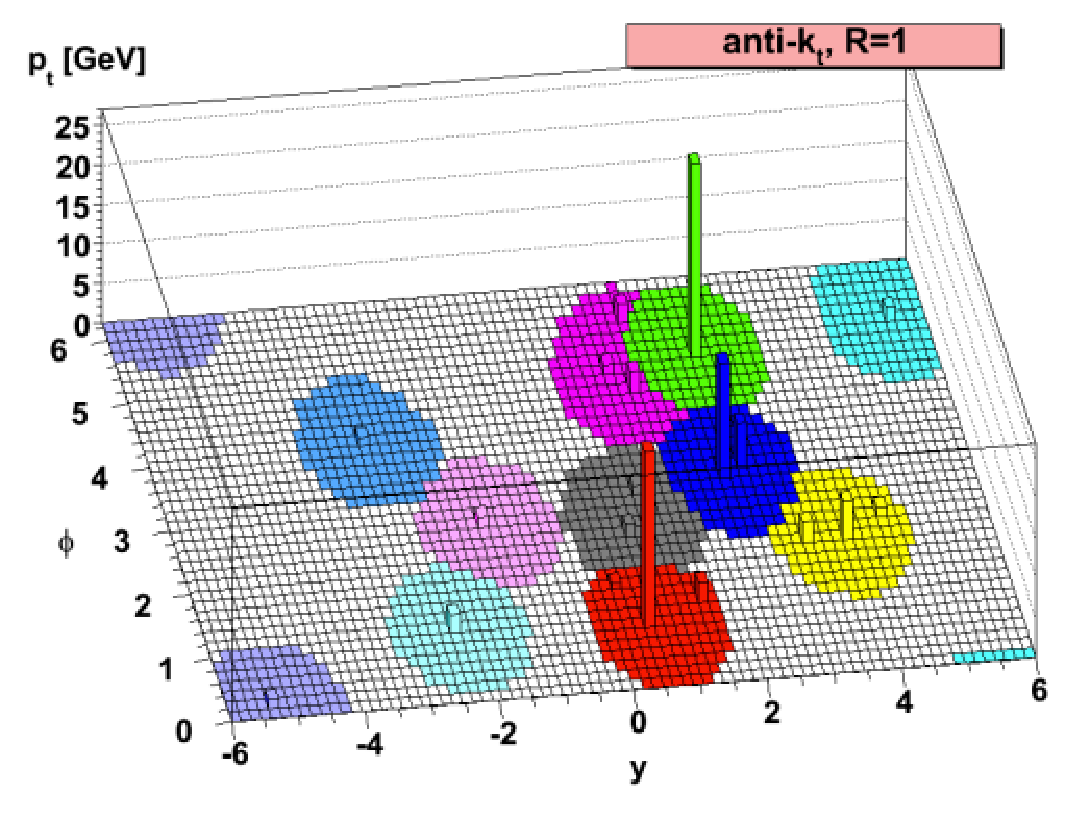
\includegraphics[width=0.45\linewidth]{{LHC_CMS/anti_kT}.pdf}
\caption[An example event of jets formed with the anti-$k_{T}$ clustering algorithm.]{An example event of jets formed with the anti-$k_{T}$ clustering algorithm\cite{Cacciari:2008gp}.}
\label{fig:anti_kT}
\end{center}
\end{figure}

In this analysis jets are only considered if they have $p_{T}^{\text{jet}} > \unit{30}{\GeV}$ and $\abs{\eta^{\text{jet}}} < 4.7$. Corrections and calibrations to the individual components of a jet according to its $p_{T}^{\text{jet}}$ and $\eta^{\text{jet}}$ following \cite{Chatrchyan:2011ds}.

\section{CMS Tracker Alignment}
\label{sec:Alignment}

The precise alignment of the silicon sensors in the CMS Tracker is a necessary and challenging task. While external measurements of the positions of sub-detectors\footnote{Using laser rays for example.} can be a good start, they are woefully inadequate in determining the exact position, tilt angle, and deformation of an individual module. In order to maximize the performance in the complex hardware that is used in the tracker the position of each module must be known to extreme precision. 

The goal of track-based alignment procedures is to determine the module positions from a large sample of reconstructed charge particle trajectories. Each trajectory is built form charge depositions on individual detectors. Using this method, the residual resolution is now below $\unit{10}{\micro\meter}$ \cite{Bayatian:922757}. This optimization problem can be formulated in the context of linear least squares. Module position corrections $\mathbf{p}$ are determined by minimizing an objective function

\begin{equation}
\label{eq:alignment}
\chi^{2}\left(\mathbf{p},\mathbf{q}\right) = \sum_{j}^{\text{tracks}}\sum_{i}^{\text{hits}}\mathbf{r}_{ij}^{T}\left(\mathbf{p},\mathbf{q}_{j}\right)\mathbf{V}_{ij}^{-1}\mathbf{r}_{ij}\left(\mathbf{p},\mathbf{q}_{j}\right),
\end{equation}

which can be expressed as a sum over all hits $i$ on all tracks $j$ and track parameters $\mathbf{q}_{j}$, assuming negligible correlations between hits. Track residuals $\mathbf{r}_{ij} = \mathbf{m}_{ij} - \mathbf{f}_{ij}\left(\mathbf{p},\mathbf{q}_{j}\right)$ are defined as the difference between the measured hit position and the estimated impact point from the trajectory without the hit in question. These residuals are given as either one- or two-dimensional vectors, and $\mathbf{V}_{ij}$ is either the squared error or the covariance matrix respectively\cite{Chatrchyan:2009sr}.

In order to determine the 200000 different parameters, \textit{alignment parameters}, that describe the locations of the 1440 silicon pixel and 15148 silicon microstrip modules two methods of minimizing track residuals are used, {\sf MILLEPEDE II} and {\sf HIP}. A \textit{track} is a fit to the series of consecutive signals that a charged particle will leave in each layer of silicon as it passes through the CMS tracker. Each of the two algorithms minimizes the residual difference between the hits that make up a track and the position of the track created without that hit. 

The main difference between the two algorithms lies in how this minimization is done. {\sf MILLEPEDE II} simultaneously determines the solutions of a complete matrix equation for global and local parameters using all tracks \cite{Blobel:2002ax}. {\sf HIP}, Hit and Impact Point, determines these parameters iteratively to solve for correlations between modules. The algorithm repeatedly fits a track and then changes a parameter, eventually minimizing the $\chi^2$ for the fit \cite{Karimaki:2006az}.

Vital to the work done as part of this thesis is the connection between the global and local parameters. The tracks and hits are defined on the module level. However these modules are connected to each other and to other subdetectors through mechanical structures that can be used to constrain the system for minimization. In figures \ref{fig:Pix_strct} and \ref{fig:Strip_strct} we map the different structures that can are used to define the locations and constraints that should be used for a given track. 


\begin{figure}
\begin{center}
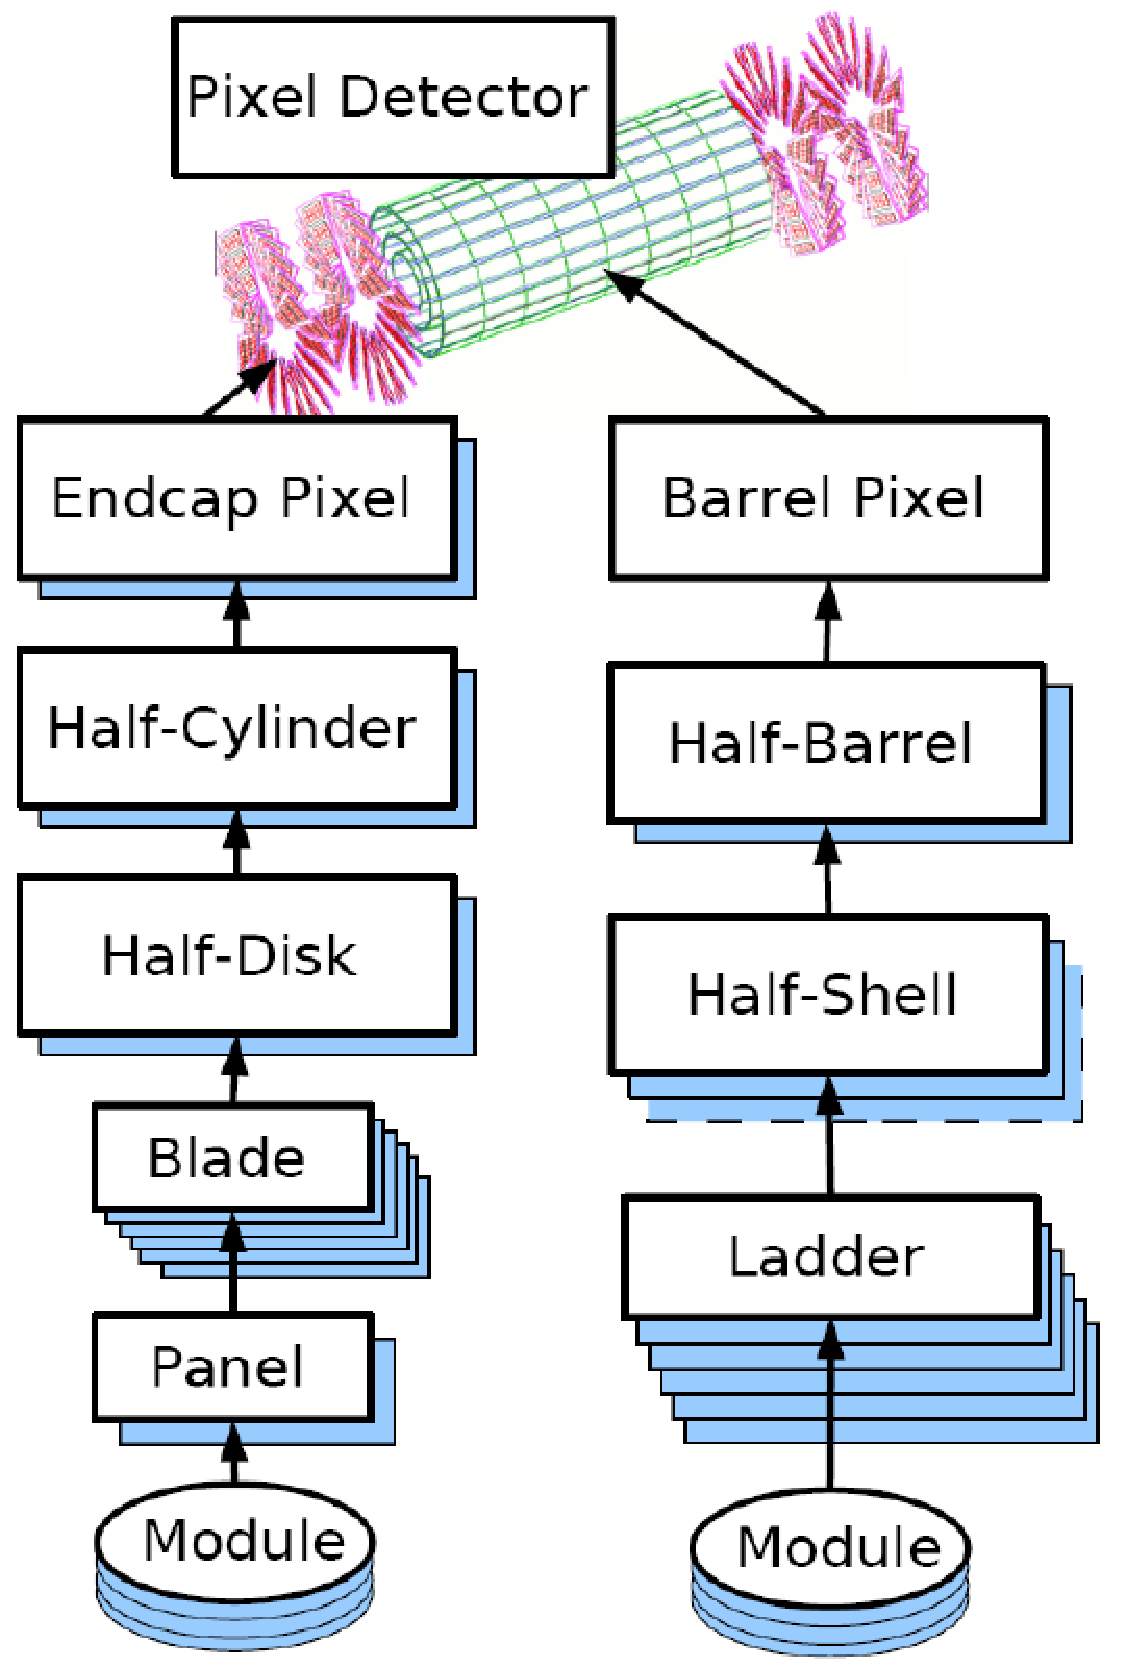
\includegraphics[width=0.45\linewidth]{{LHC_CMS/Pix_strct}.pdf}
\caption[Hierarchy of the CMS silicon pixel detector structures.]{Hierarchy of the CMS silicon pixel detector structures\cite{CMS-doc-1157-v7}.}
\label{fig:Pix_strct}
\end{center}
\end{figure}

\begin{figure}
\begin{center}
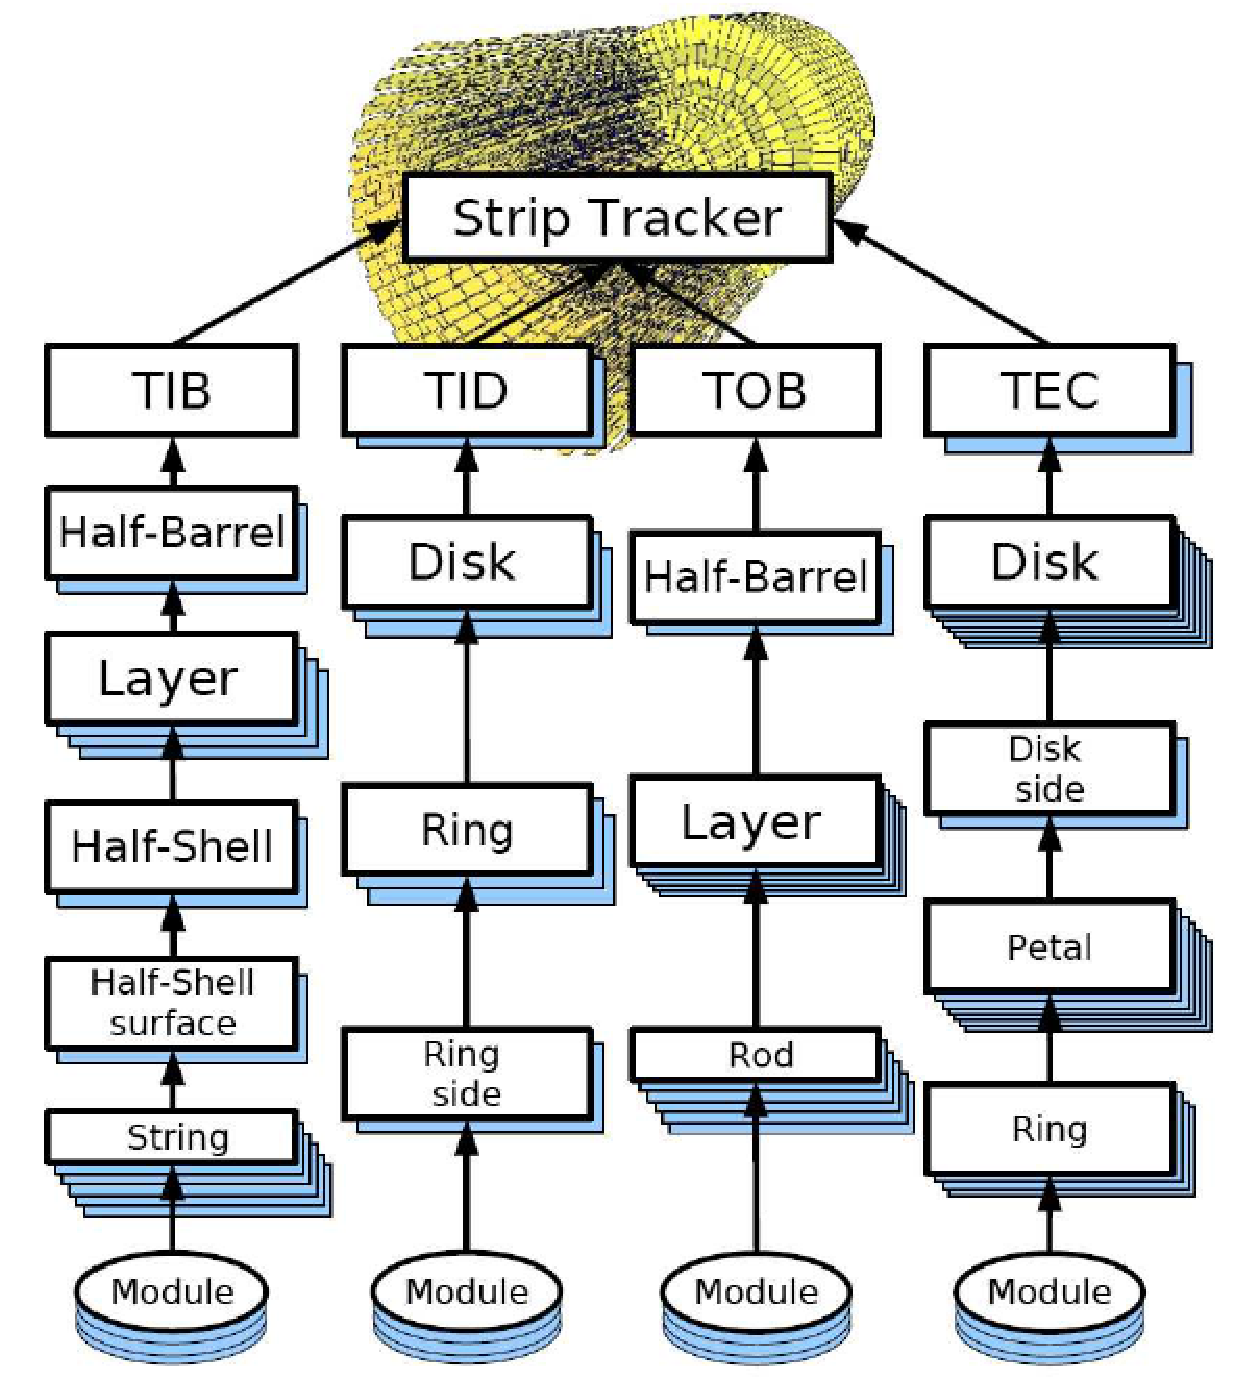
\includegraphics[width=0.45\linewidth]{{LHC_CMS/Strip_strct}.pdf}
\caption[Hierarchy of the CMS silicon strip detector structures.]{Hierarchy of the CMS silicon strip detector structures\cite{Adam:2009aa}.}
\label{fig:Strip_strct}
\end{center}
\end{figure}

\subsection{Silicon Pixel Alignment in Prompt Calibration Loop}
Once a set of alignment parameters is determined, it is not valid forever. As the detector operates the different components may shift. A prime example of this is the pixel barrel, which is not in a fixed position. This is problematic because the CMS magnet may turn on and off, resulting in natural shifts in the positions of different detectors. Part of this thesis work was to develop and implement an active alignment algorithm that would detect and automatically update the detector positions as the CMS experiment takes data.

This active alignment algorithm was implemented in the CMS tracker Prompt Calibration Loop for the start of the 2015 run of the LHC. The Prompt Calibration Loop is a collection of routines that are designed to monitor and automatically adjust parameters to optimize the performance of the the CMS tracking system. The alignment routine developed during this thesis work monitors and adjusts the 36 alignment parameters that describe the pixel detector global parameters. The monitored parameters are the positions $\left(x, y, z\right)$ and rotations $\left(\theta_{x}, \theta_{y}, \theta_{z}\right)$ of the two BPIX half-barrels and the four half-cylinders of the FPIX system\footnote{Two half-cylinders each for FPIX+ and FPIX-.}. If a sufficient shift in one of these parameters is seen\footnote{In this case, ``sufficient" implies the parameter shifts between a pre-set minimum and maximum window and the significance of that shift is larger than a pre-set amount.} then the database of tracker conditions is updated. These consistent updates allow CMS to continue operating at peak performance and avoids rerunning computationally expensive data processing routines to correct the data after the fact. 

The effectiveness of this project is illustrated from similar algorithm that was used at the end of the 2012 run after a large shift in the pixel barrel position was seen. Figure \ref{fig:2011PixelShift} shows the longitudinal shift between the two half-shelf of the BPIX as measured with the primary vertex residuals. The previous monitoring procedure was implemented farther `downstream' in the computing chain than the current implementation.

\begin{figure}
\begin{center}
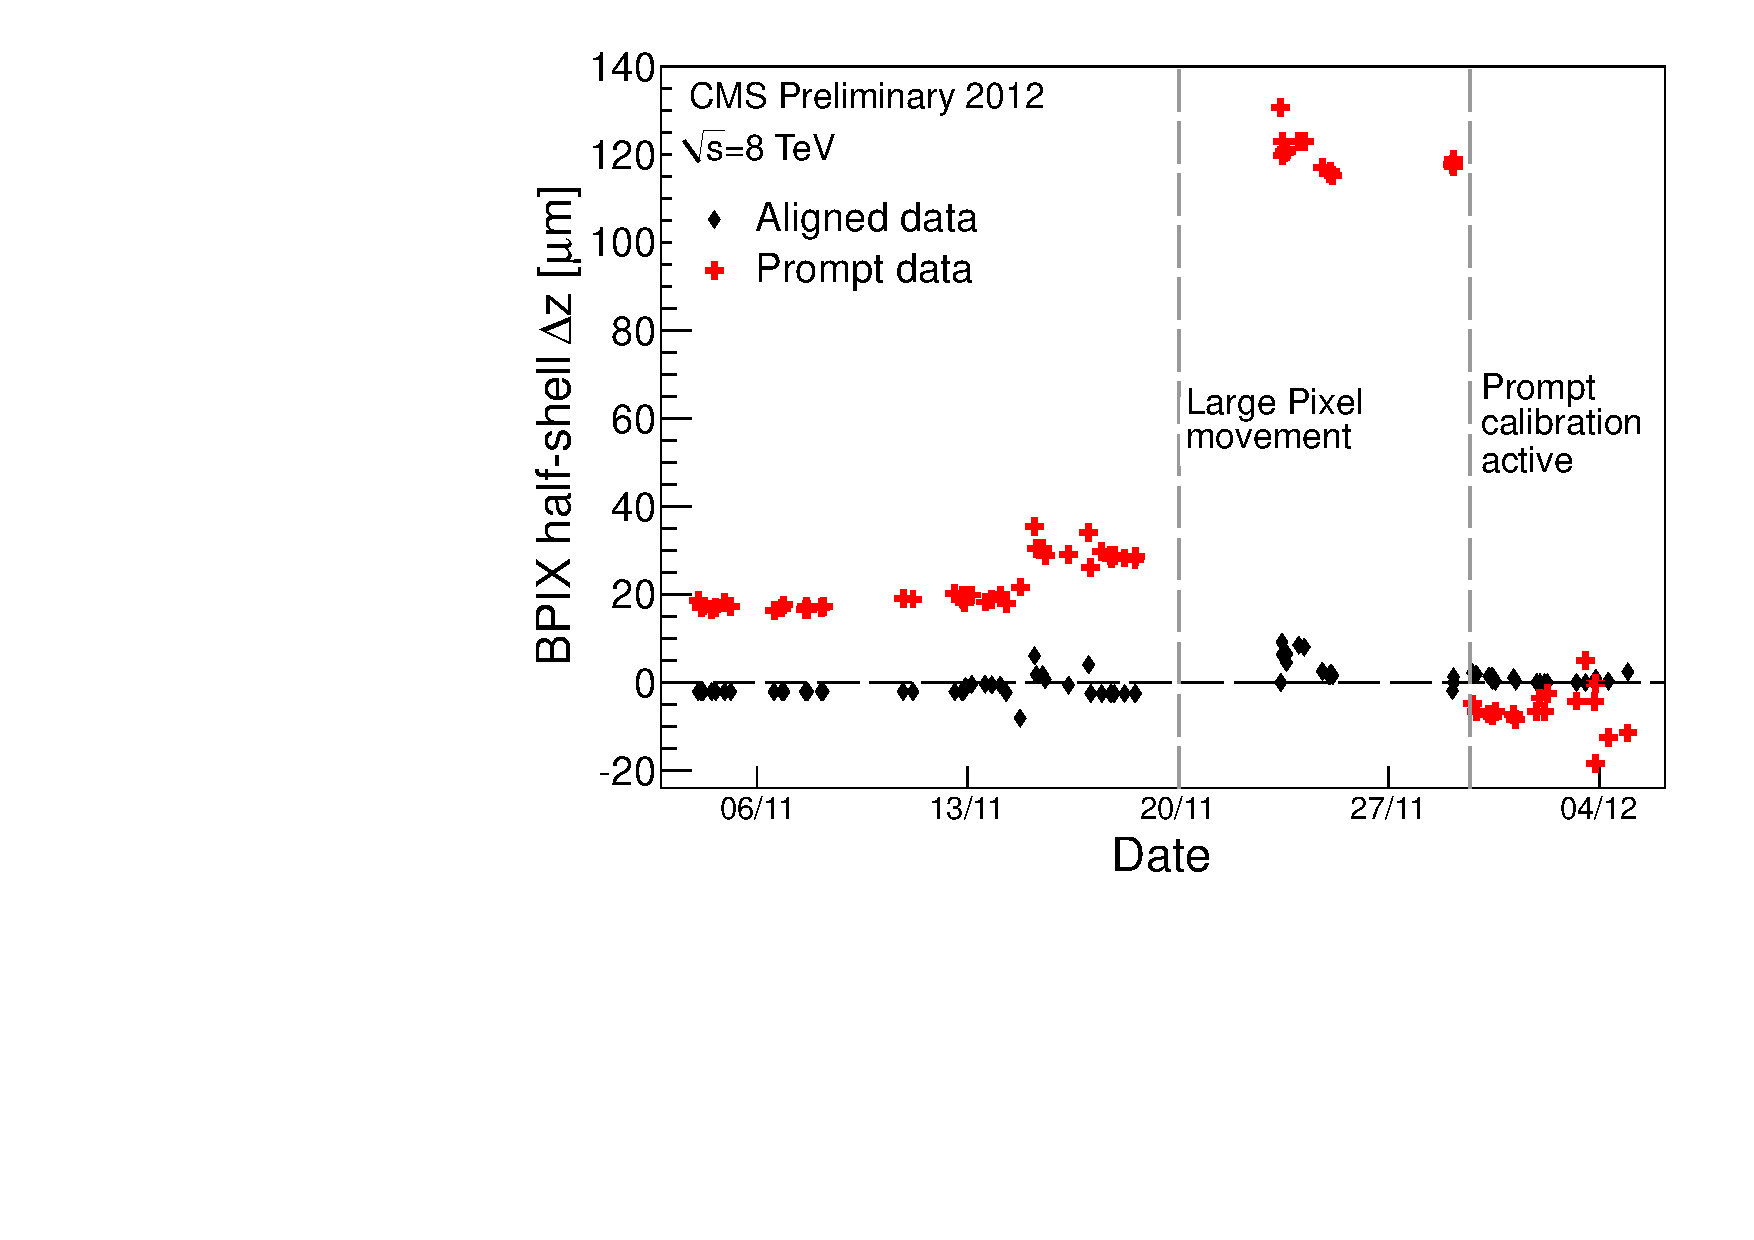
\includegraphics[width=.65\linewidth]{{LHC_CMS/PCL_lateNovRuns}.pdf}
\caption[Day-by-day value of the relative longitudinal shift between the two half-shells of the BPIX as measured with the primary vertex residuals, for the last month of pp data taking in 2012. Red crosses show the shift observed using the data coming from the prompt reconstruction. The same events, re-reconstructed after the 2012 alignment campaign, which accounts for the major changes in the positions of the half-shells, are represented by black lozenges. A major displacement of the half-shells O(100) $\micro\meter$, occurred during the technical stop in the week of 20th of November, is recovered by the prompt alignment of the BPIX large structures that became active on the 30th November.]{Day-by-day value of the relative longitudinal shift between the two half-shells of the BPIX as measured with the primary vertex residuals, for the last month of pp data taking in 2012. Red crosses show the shift observed using the data coming from the prompt reconstruction. The same events, re-reconstructed after the 2012 alignment campaign, which accounts for the major changes in the positions of the half-shells, are represented by black lozenges. A major displacement of the half-shells O(100) $\micro\meter$, occurred during the technical stop in the week of 20th of November, is recovered by the prompt alignment of the BPIX large structures that became active on the 30th November \cite{CMS-DP-2013-017}.}
\label{fig:2011PixelShift}
\end{center}
\end{figure}

\chapter{Higgs boson at the LHC: Phenomenology}
\label{sec:LHC_Pheno}
\chaptermark{Higgs boson at the LHC: Phenomenology}


In this section we discuss specific phenomenological details that are studied for this thesis. First, we discuss the different modes of producing a Higgs boson at the LHC, and different features of these different production modes. Next, we will present the decay of a Higgs boson into two Z bosons and subsequently four leptons. Using this information we will present the implications of off resonance production and decay on the Higgs boson lifetime. Finally, we will discuss the spin and parity of a single-produced resonance and how we can use these relations to characterize a new particle found at the LHC.

\section{Higgs boson production at LHC}
\label{sec:Higgs_Production_Pheno}

In proton-proton collisions a SM Higgs boson can be produced through the coupling of a Higgs boson to either bosons or fermions. Each of these two categories of Higgs boson production will be dominated by specific production modes. Fermionic production of a Higgs boson can happen either through \textit{gluon-gluon fusion} $gg \to H$ (ggH) and much less frequently through production in \textit{association with two top quarks} $gg \to H + t\bar{t}$ ($t\bar{t}H$). Bosonic production of a Higgs boson can occur through \textit{vector boson fusion} (VBF), where two quarks radiate vector bosons which produce the boson in association with two quark jets $qq \to H + 2\text{jets}$ or through production \textit{associated with a vector boson} $qq \to H + W/Z$ (VH).

The cross sections of these different production mechanisms as a function of the Higgs boson mass at the LHC are shown in figure \ref{fig:LHC_Hxsec} for the two center of mass energies used in this thesis; $\sqrt{s} = \unit{7}{\TeV}$ and $\sqrt{s} = \unit{8}{\TeV}$ \cite{Dittmaier:2011ti, Dittmaier:2012vm}. Notable features of these cross sections are the order of magnitude difference between gluon-gluon fusion and the bosonic production modes which are all much larger than the $H + t\bar{t}$ production. Additionally, one can see the boost in the gluon-gluon fusion production at $2m_{t}$, which corresponds to the top quark in the production loop going becoming on shell (explained in more detail below).

\begin{figure}
\begin{center}
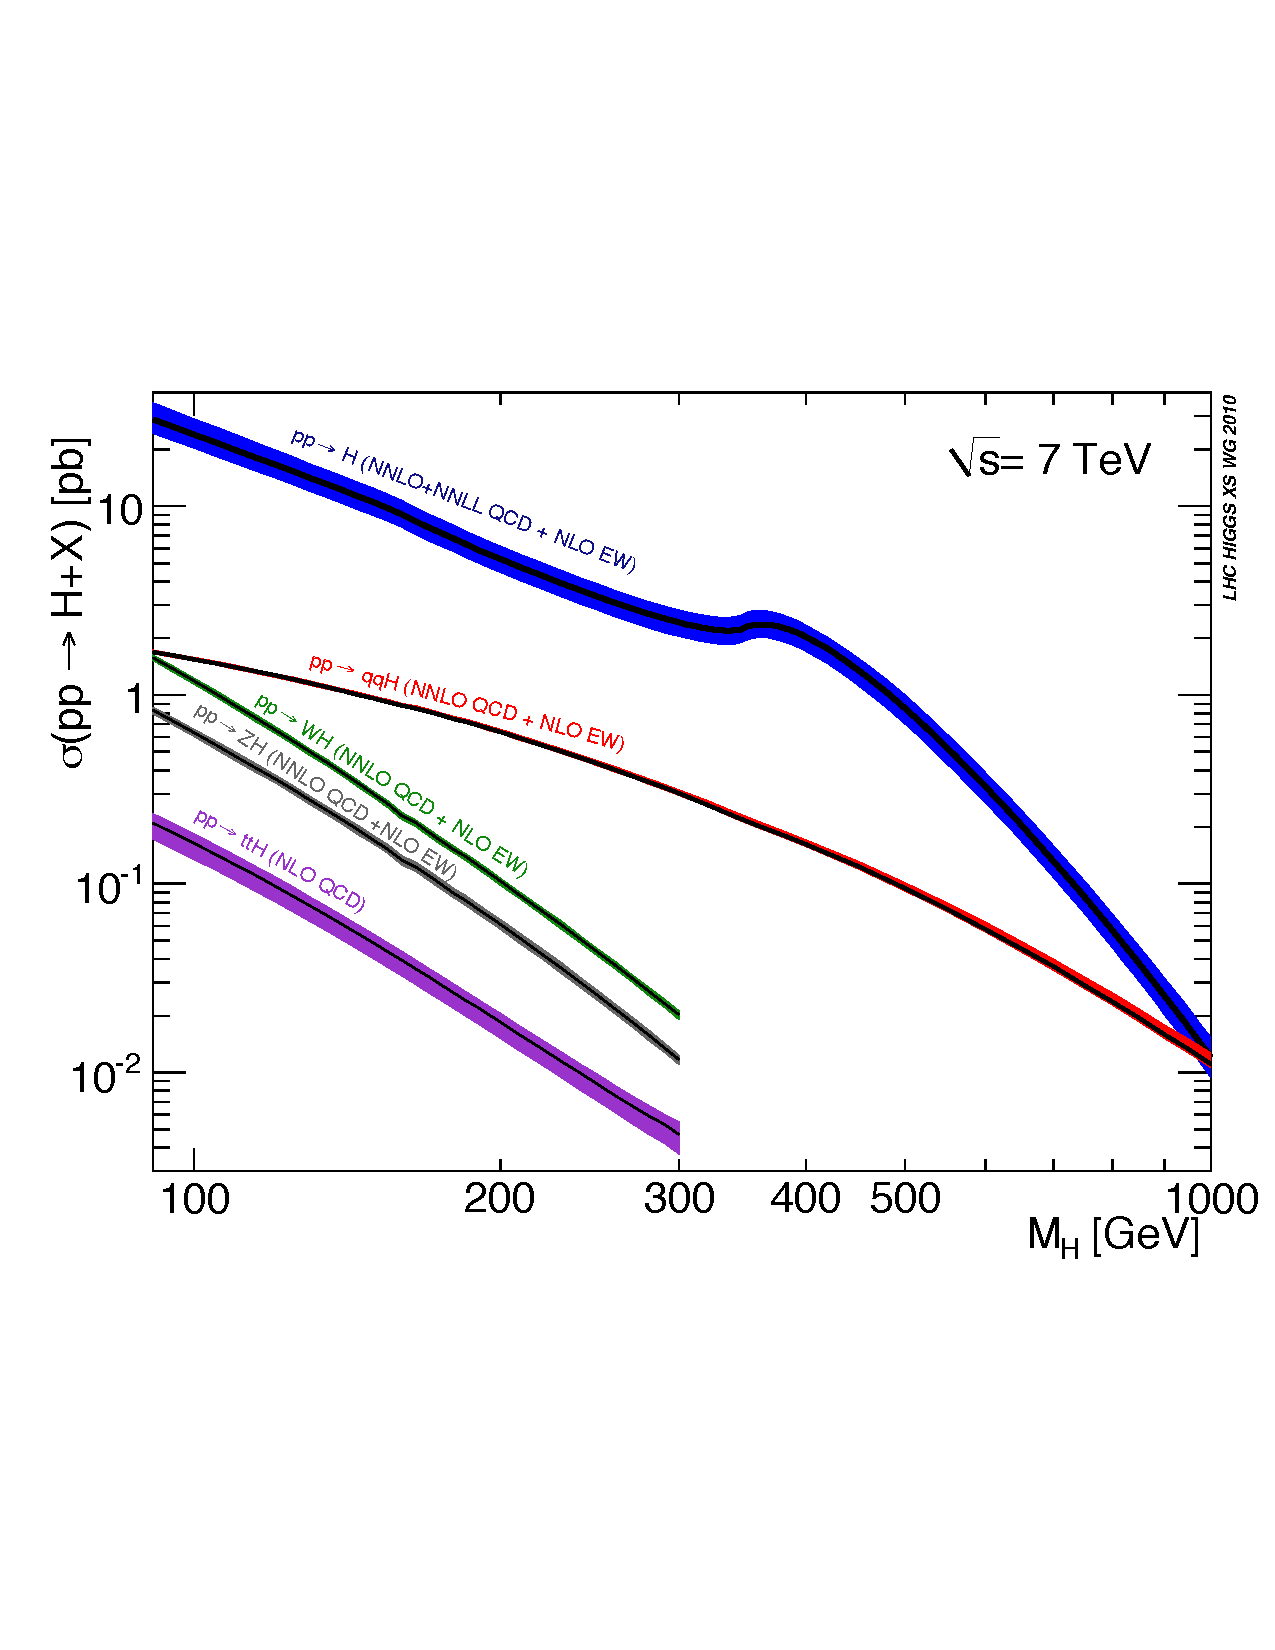
\includegraphics[width=0.46\linewidth]{{LHC_Pheno/Higgs_XS_7TeV}.pdf}
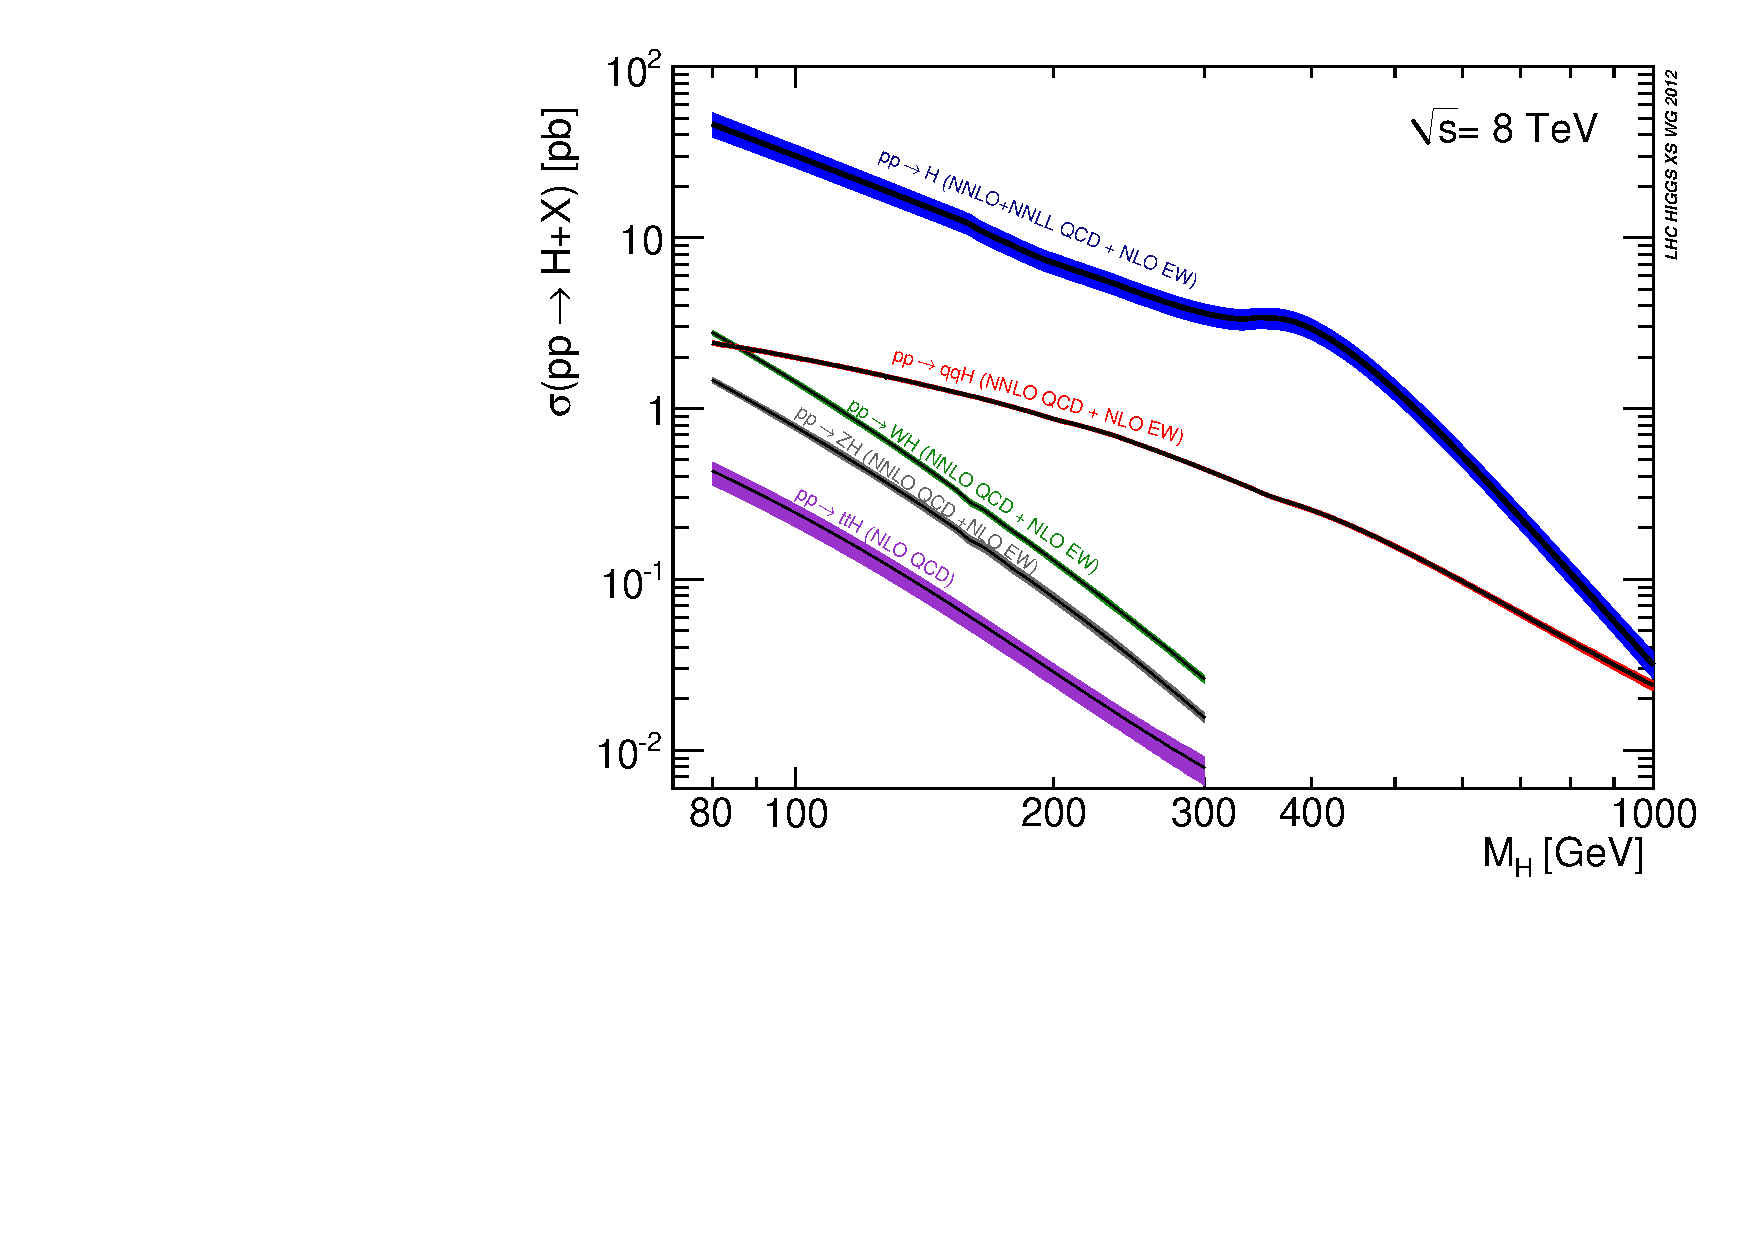
\includegraphics[width=0.455\linewidth]{{LHC_Pheno/Higgs_XS_8TeV_lx}.pdf}
\caption[Standard Model Higgs boson production cross sections and relative uncertainties at $\sqrt{s} = \unit{7}{\TeV}$ and $\sqrt{s} = \unit{8}{\TeV}$. From top to bottom these are $pp \to H$, blue, $pp \to H + 2\text{jets}$, red, $pp \to H + W$, green, $pp \to H + Z$, grey, $pp \to H + t\bar{t}$, purple.]{Standard Model Higgs boson production cross sections and relative uncertainties at $\sqrt{s} = \unit{7}{\TeV}$ and $\sqrt{s} = \unit{8}{\TeV}$. From top to bottom these are $pp \to H$, blue, $pp \to H + 2\text{jets}$, red, $pp \to H + W$, green, $pp \to H + Z$, grey, $pp \to H + t\bar{t}$, purple \cite{Dittmaier:2011ti, Dittmaier:2012vm}.}
\label{fig:LHC_Hxsec}
\end{center}
\end{figure}

The main production mechanism at the LHC is gluon-gluon fusion. The Feynman diagram for this process is shown in figure \ref{fig:ggH_Feyn}. While the Higgs boson does not couple directly to gluons (because they are massless) this mode of production relies on the Higgs boson coupling to fermions generated by the incoming gluons. Because the coupling of the Higgs boson is proportional to the mass of the fermion the dominant contribution is the Higgs boson -- top coupling. This leads to a boost in the cross section when the mass of the Higgs boson is twice the top mass because the top in the loop shown is no longer virtual. For the entire mass range that is considered in this analysis this is the most common way to produce a Higgs boson at the LHC.

\begin{figure}
\begin{center}
\unitlength=1mm
\begin{fmffile}{ggH_Feyn}

\begin{fmfgraph*}(40,30) 
  \fmfleft{i1,i2} \fmfright{sp1}
  \fmf{gluon,label=$g$}{i1,v1} 
  \fmf{gluon,label=$g$}{i2,v2}
  \fmf{fermion}{v1,v2,v3,v1}
  \fmffixed{(0,.6h)}{v1,v2}
  \fmf{dashes,label=$H$}{v3,sp1}
\end{fmfgraph*}

\end{fmffile}
\end{center}
\caption[Feynman diagram depicting Higgs boson production through gluon-gluon fusion $gg \to H$. The fermion loop is dominated by top quarks, however all quarks contribute according to their masses.]{Feynman diagram depicting Higgs boson production through gluon-gluon fusion $gg \to H$. The fermion loop is dominated by top quarks, however all quarks contribute according to their masses.}
\label{fig:ggH_Feyn}
\end{figure}

The second most likely way to produce a Higgs boson at the LHC is through vector boson fusion. To produce a Higgs boson this way two quarks each radiate a W or Z boson which fuse into the Higgs boson. This production mode relies on the Higgs boson coupling to the vector bosons, making it distinct compared to gluon-gluon fusion. the distinguishing feature of this production mode is the presence of two quark jets in the final state in addition to the Higgs boson. These jets contain information about the Higgs boson and can be exploited to refine searches and study the properties of a new particle. The Feynman diagram for this process is shown in figure \ref{fig:qqH_Feyn}.

\begin{figure}
\begin{center}
\unitlength=1mm
\begin{fmffile}{qqH_Feyn}

\begin{fmfgraph*}(40,30) 
  \fmfleft{i1,i2} \fmfright{sp1,sp2,sp3}
  \fmf{fermion,label=$q$}{i1,v1,sp1} 
  \fmf{fermion,label=$q$}{i2,v2,sp3}
  \fmf{boson,label=$W/Z$,label.side=left}{v1,v3}
  \fmf{boson}{v3,v2}
  \fmffixed{(0,.3h)}{v1,v3}
  \fmffixed{(0,.3h)}{v3,v2}
  \fmf{dashes,label=$H$}{v3,sp2}
\end{fmfgraph*}

\end{fmffile}
\end{center}
\caption[Feynman diagram depicting Higgs boson production through vector boson fusion $qq \to H + 2\text{jets}$.]{Feynman diagram depicting Higgs boson production through vector boson fusion $qq \to H + 2\text{jets}$.}
\label{fig:qqH_Feyn}
\end{figure}

Sub-dominant to these two production modes are processes that produce a Higgs boson in association with vector bosons or top quarks. This thesis does not tune the analysis to separate these modes from the dominant ones, instead they are grouped with the dominant modes by how the Higgs boson couples to the other standard model particles. VBF is grouped with VH because the Higgs boson is produced through a coupling to vector bosons while $t\bar{t}H$ is grouped with ggH because it relies on the Higgs boson coupling to fermions.

Producing the Higgs boson in association with a W or Z boson is conceptually similar to VBF production. Two quarks interact, producing a vector boson which radiates away a Higgs boson, shown in figure \ref{fig:VH_Feyn}. Unique to this final state is that in addition to the Higgs boson you will also have the particles associated with the subsequent decay of a W or Z boson. The $t\bar{t}H$ production mode is the smallest of those considered here and is similar to ggH in that it relies on the Higgs boson coupling to top quarks. While the rates of $t\bar{t}H$ are very low, Higgs bosons produced in this way can be distinguished by the presence of two top quarks in addition to the decay product of the Higgs boson, as shown in figure \ref{fig:ttH_Feyn}.

\begin{figure}
\begin{center}
\unitlength=1mm
\begin{fmffile}{VH_Feyn}

\begin{fmfgraph*}(40,30) 
  \fmfleft{i1,i2} \fmfright{sp1,sp2}
  \fmf{fermion,label=$q$}{i1,v1,i2} 
  \fmf{boson}{v1,v3}
  \fmf{boson,label=$W/Z$}{v3,sp1}
  \fmffixed{(.3w,0)}{v1,v3}
  \fmf{dashes,label=$H$}{v3,sp2}
\end{fmfgraph*}

\end{fmffile}
\end{center}
\caption[Feynman diagram depicting Higgs boson production associated with a vector boson $qq \to H + W/Z$.]{Feynman diagram depicting Higgs boson production associated with a vector boson $qq \to H + W/Z$.}
\label{fig:VH_Feyn}
\end{figure}

\begin{figure}
\begin{center}
\unitlength=1mm
\begin{fmffile}{ttH_Feyn}

\begin{fmfgraph*}(40,30) 
  \fmfleft{i1,i2} \fmfright{sp1,sp2,sp3}
  \fmf{gluon,label=$g$}{i1,v1} 
  \fmf{gluon,label=$g$}{i2,v2}
  \fmf{fermion,label=$t$}{sp1,v1}
  \fmf{fermion}{v1,v3,v2}
  \fmf{fermion,label=$t$}{v2,sp3}
  \fmffixed{(0,.3h)}{v1,v3}
  \fmffixed{(0,.3h)}{v3,v2}
  \fmf{dashes,label=$H$}{v3,sp2}
\end{fmfgraph*}

\end{fmffile}
\end{center}
\caption[Feynman diagram depicting Higgs boson production in association with two top quarks $gg \to H + t\bar{t}$.]{Feynman diagram depicting Higgs boson production in association with two top quarks $gg \to H + t\bar{t}$.}
\label{fig:ttH_Feyn}
\end{figure}

More details are presented in section \ref{sec:prod_dec_frac}, this thesis uses the different properties of ggH and VBF production modes to measure how often a Higgs boson is produced in each mode at the LHC. This work resulted in the first measurement of the production mechanism of Higgs bosons in the $4\ell$ final state.

\section{Higgs boson decay to \texorpdfstring{$ZZ \to 4\ell$}{ZZ to 4l}}
\label{sec:Higgs_Decay_ZZ_4l}

The SM Higgs boson is an unstable particle that will decay before it can be detected with the CMS detector. However, we can search for this particle by looking at its decay products. To determine which decay products will be the most fruitful to use for a search, we look at the \textit{branching ratio} $BR_{X} = \frac{N_{X}}{N_{tot}}$ of the Higgs boson decay for a specific final state in relation to the total number of Higgs bosons we expect. Thus, a high branching ratio will result in a larger number of signal events. In figure \ref{fig:Higgs_BR} we plot some of the interesting branching ratios as a function of the Higgs boson mass. To decide if a search is valuable we compare the number of events we expect from a specific decay mode (given by the luminosity times branching ratio times the cross section $\mathcal{L}\cdot BR_{X}\cdot\sigma_{tot}$) to the number of background events we expect in the search range.

\begin{figure}
\begin{center}
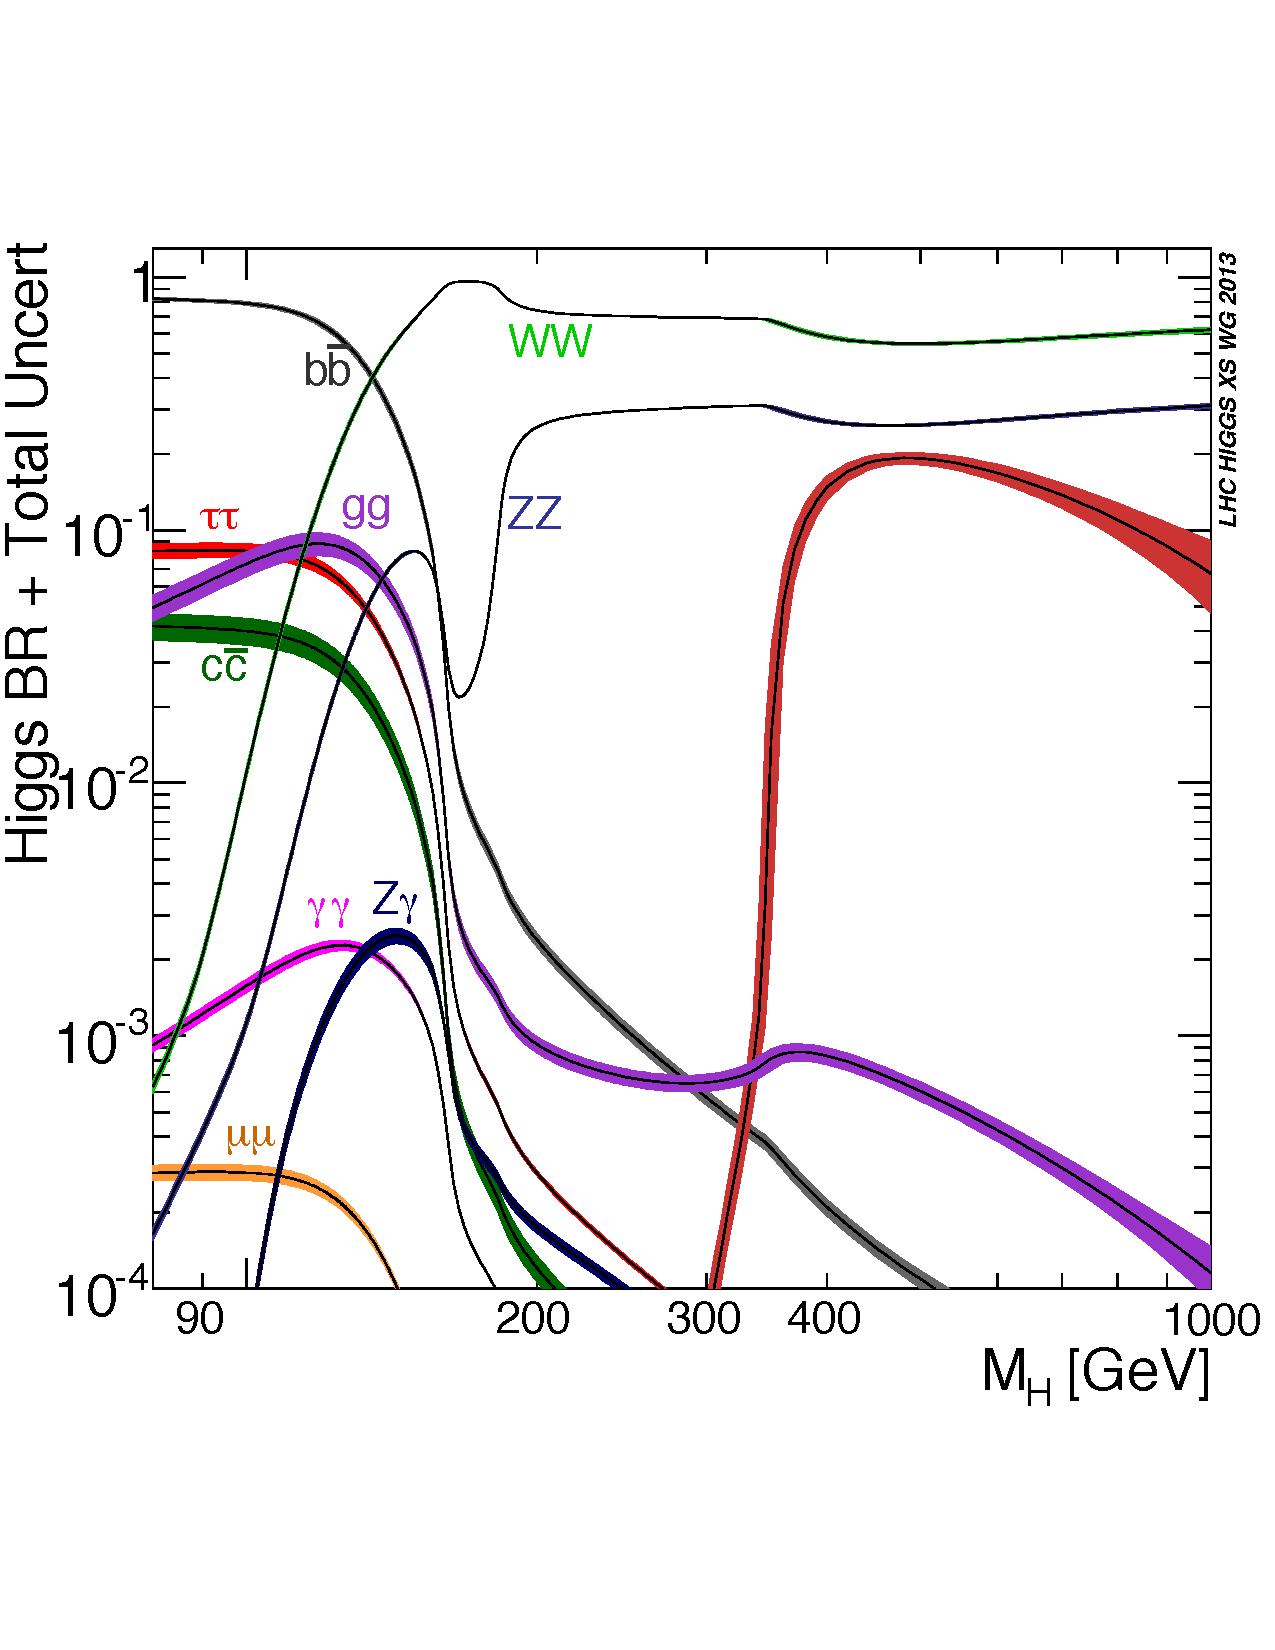
\includegraphics[width=0.45\linewidth]{{LHC_Pheno/Higgs_BR}.pdf}
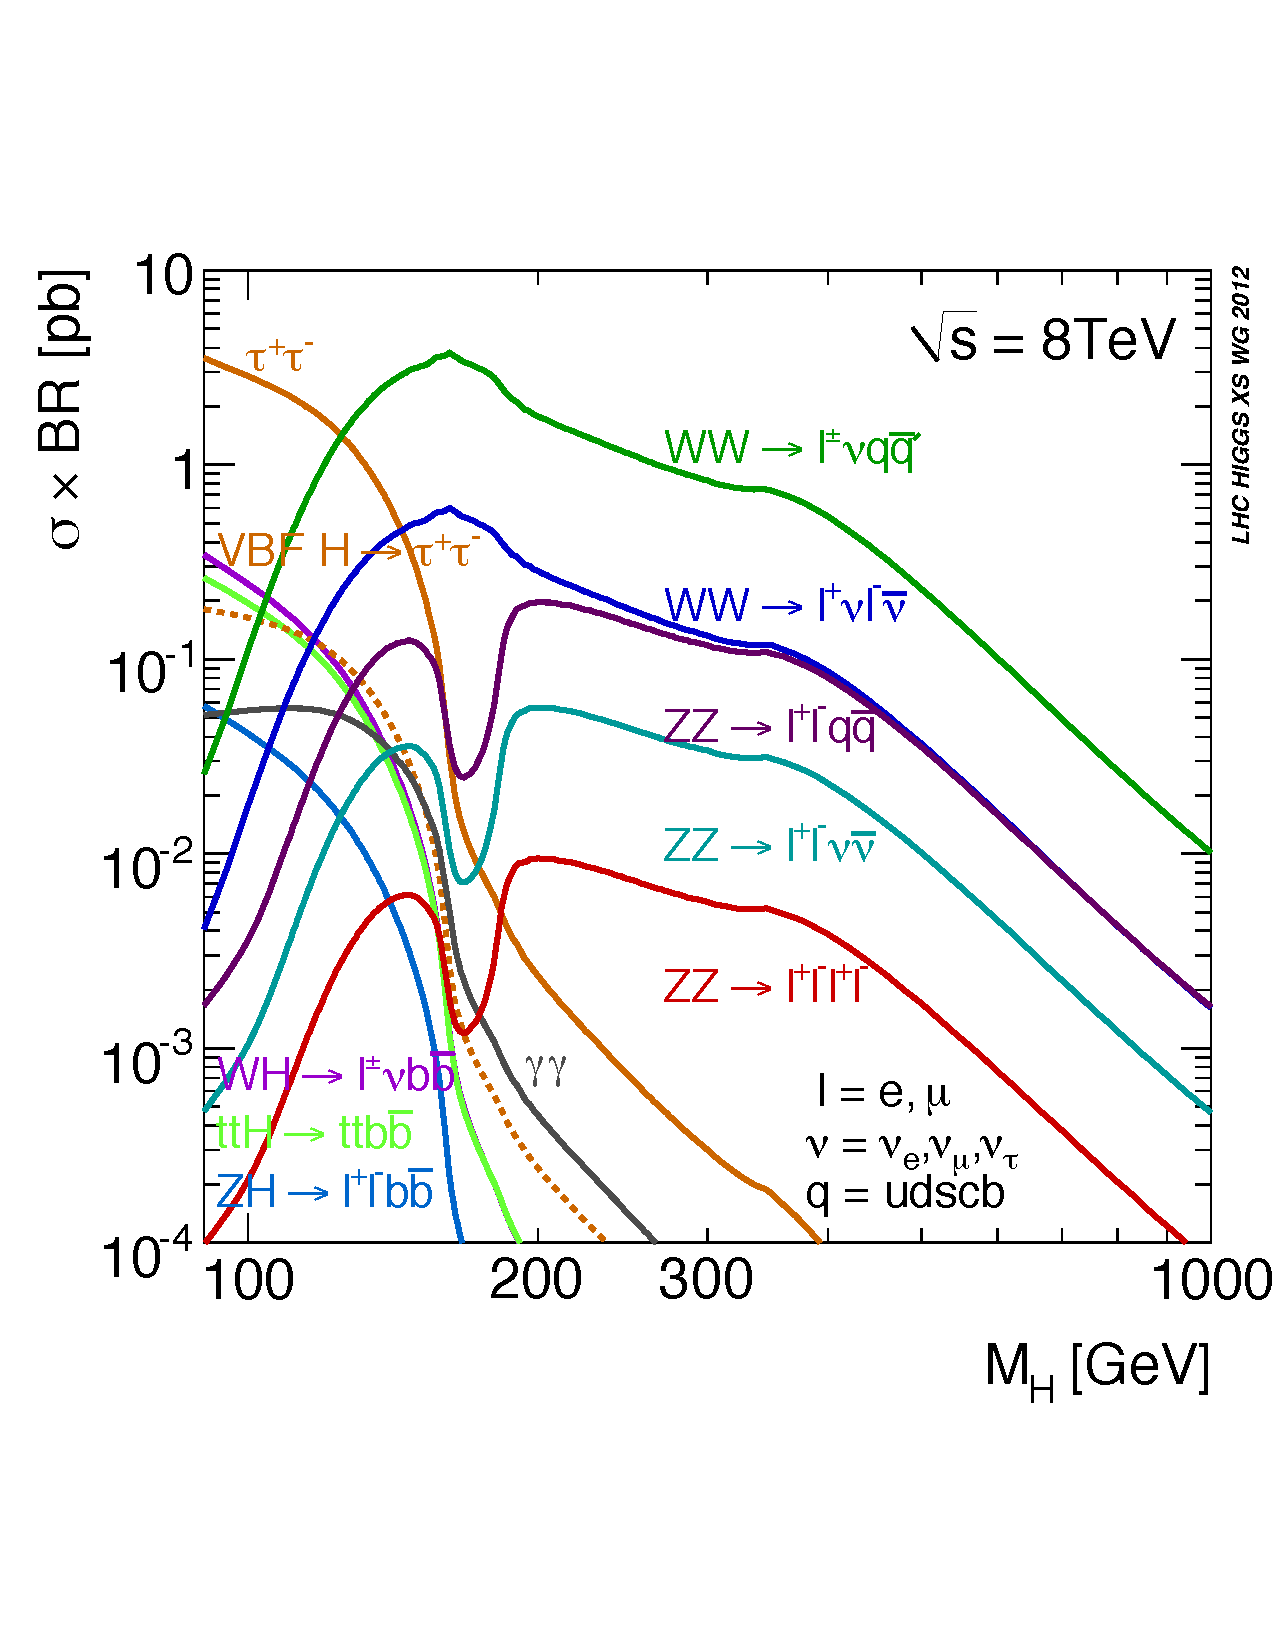
\includegraphics[width=0.46\linewidth]{{LHC_Pheno/XSBR_8TeV_SM_HM}.pdf}
\caption[(left) Standard Model Higgs boson decay branching ratios for selected decay modes, of specific interest for this thesis is the $ZZ$ branching ratio. (right) Branching ratio times cross section for selected final states, of specific interest for this thesis is the $ZZ \to 4\ell\left(\ell^{+}\ell^{-}\ell^{+}\ell^{-}\right)$.]{(left) Standard Model Higgs boson decay branching ratios for selected decay modes, of specific interest for this thesis is the $ZZ$ branching ratio. (right) Branching ratio times cross section for selected final states, of specific interest for this thesis is the $ZZ \to 4\ell\left(\ell^{+}\ell^{-}\ell^{+}\ell^{-}\right)$\cite{Dittmaier:2012vm, Heinemeyer:2013tqa}.}
\label{fig:Higgs_BR}
\end{center}
\end{figure}

Of specific interest for this thesis is the Higgs boson decay to the $ZZ \to 4\ell$ final state, shown in figure \ref{fig:H_ZZ_4l_Feyn}. Where we consider $\ell = e, \mu$ because these leptons will be long lived enough to be detected directly by CMS, making them distinct from $\tau$ leptons which often decay because of their high mass. The $ZZ$ branching ratio is one of the highest across a wide rage of possible Higgs boson masses, making it advantageous for search and characterization studies. The $4\ell$ final state is used not because it has a particularly high cross section times branching ratio (seen in figure \ref{fig:Higgs_BR} right), but because there are low SM background contributions and because all of the final particles are directly detected by the CMS detector.

\begin{figure}
\begin{center}
\unitlength=2mm
\begin{fmffile}{H_ZZ_4l_Feyn}
\begin{fmfgraph*}(40,30) 
  \fmfleft{i1} \fmfright{sp1,sp2,sp3,sp4}
  \fmf{dashes,label=$H$}{i1,v1} 
  \fmf{boson,label=$Z$}{v1,v2}
  \fmf{boson,label=$Z$}{v1,v3}
  \fmf{fermion,label=$e/\mu$}{sp1,v2,sp2}
  \fmf{fermion,label=$e/\mu$}{sp3,v3,sp4}
\end{fmfgraph*}

\end{fmffile}
\end{center}
\caption[Feynman diagram depicting Higgs boson decay into two Z bosons and subsequently into four leptons $H \to ZZ \to 4\ell$.]{Feynman diagram depicting Higgs boson decay into two Z bosons and subsequently into four leptons $H \to ZZ \to 4\ell$.}
\label{fig:H_ZZ_4l_Feyn}
\end{figure}

This thesis considers all of the data collected by CMS during run 1 of the LHC proton-proton collisions. This corresponds to an integrated luminosity of $\unit{5.1}{\invfemtobarn}$ collected at a center of mass energy of $\sqrt{s} = \unit{7}{\TeV}$ and $\unit{19.7}{\invfemtobarn}$ collected at $\sqrt{s} = \unit{8}{\TeV}$. The search for and later characterization of a Higgs boson requires that there be two pairs of same-flavor, opposite-charge, well-identified isolated leptons $\left(e^{+}e^{-}e^{+}e^{-}, \mu^{+}\mu^{-}\mu^{+}\mu^{-}, \text{ or } e^{+}e^{-}\mu^{+}\mu^{-}\right)$ compatible with an intermediate state of $ZZ$. Computability with $ZZ$ is defined such that one or both of the $Z$'s can be off the mass resonance of the Z-boson.

In this case, a Higgs boson signal will appear as a narrow mass peak on top of a smooth background when observing the four lepton mass distribution. The search is conducted in a mass range of $m_{4\ell} \in \unit{110 -- 1000}{\GeV}$. For low-mass Higgs bosons $\left(m_{H} < \unit{400}{\GeV}\right)$, the width of the resonance in $m_{4\ell}$ is very well peaked and described with a Breit-Wigner distribution. For higher mass Higgs bosons $\left(m_{H} > \unit{400}{\GeV}\right)$, the width of the $m_{4\ell}$ mass peak is much broader and described in the complex pole scheme \cite{Dittmaier:2011ti, Dittmaier:2012vm, Heinemeyer:2013tqa}. Detailed analysis of the width of the Higgs boson will be discussed in section \ref{sec:Higgs_Width_Pheno}.

\begin{figure}
\begin{center}
\unitlength=2mm
\begin{fmffile}{qq_ZZ_4l_Feyn}
\begin{fmfgraph*}(40,15) 
  \fmfleft{i1,i2} \fmfright{sp1,sp2,sp3,sp4}
  \fmf{fermion,label=$q$}{i1,v1,v2,i2} 
  \fmffixed{(.3w,0)}{i1,v1}
  \fmffixed{(.3w,0)}{i2,v2}
  %\fmffixed{(0,.3h)}{v2,v1}
  \fmf{boson,label=$Z$}{v1,v3}
  \fmf{boson,label=$Z$}{v2,v4}
  \fmffixed{(.3w,0)}{v1,v3}
  \fmffixed{(.3w,0)}{v2,v4}
  %\fmf{fermion,label=$e/\mu$}{sp1,v3,sp2}
  %\fmf{fermion,label=$e/\mu$}{sp3,v4,sp4}
\end{fmfgraph*}

\end{fmffile}
\end{center}
\caption[Feynman diagram depicting the quark production of two Z bosons $qq \to ZZ$.]{Feynman diagram depicting the quark production of two Z bosons $qq \to ZZ$.}
\label{fig:qq_ZZ_4l_Feyn}
\end{figure}

\begin{figure}
\begin{center}
\unitlength=2mm
\begin{fmffile}{gg_ZZ_4l_Feyn}
\begin{fmfgraph*}(40,15) 
  \fmfleft{i1,i2} \fmfright{sp1,sp2,sp3,sp4}
  \fmf{gluon,label=$g$}{i1,v1} 
  \fmf{gluon,label=$g$}{i2,v2} 
  \fmffixed{(.3w,0)}{i1,v1}
  \fmffixed{(.3w,0)}{i2,v2}
  \fmf{fermion,label=$q$}{v1,v2,v3,v4,v1}
  \fmffixed{(.3w,0)}{v2,v3}
  \fmffixed{(.3w,0)}{v1,v4}
  \fmf{boson,label=$Z$}{v3,v5}
  \fmf{boson,label=$Z$}{v4,v6}
  \fmffixed{(.3w,0)}{v3,v5}
  \fmffixed{(.3w,0)}{v4,v6}
  %\fmf{fermion,label=$e/\mu$}{sp1,v6,sp2}
  %\fmf{fermion,label=$e/\mu$}{sp3,v5,sp4}
\end{fmfgraph*}

\end{fmffile}
\end{center}
\caption[Feynman diagram depicting the gluon production of two Z bosons $gg \to ZZ$.]{Feynman diagram depicting the gluon production of two Z bosons $gg \to ZZ$.}
\label{fig:gg_ZZ_4l_Feyn}
\end{figure}

The background in the $4\ell$ final state is dominated by the SM $q\bar{q} \to ZZ \to 4\ell$ production, shown in figure \ref{fig:qq_ZZ_4l_Feyn}. This background is not particularly large but it cannot be reduced with quality cuts on the leptons or tuning of phase space without significant losses to the expected signal. Additionally, there will be SM $gg \to ZZ \to 4\ell$, shown in figure \ref{fig:gg_ZZ_4l_Feyn}. Z boson production from gluons is also irreducible, but this contribution is about 10\% of the dominant $qq \to ZZ \to 4\ell$ production. As discussed in the next section, this $gg \to ZZ$ contribution can actually be exploited to study the properties of any new resonance. There will also be background contributions from collisions that produce a Z boson in addition to other jets or particles that are mis-identified as leptons. This background is reducible by tuning the analysis to remove as much of this noise as possible. This tuning is done by adjusting the quality requirements on the leptons and requirements about where the events fall in phase space. This process is described more in section \ref{sec:BkgEstimation}.

\section{Higgs boson width: off resonance production and decay}
\label{sec:Higgs_Width_Pheno}

When a new particle is observed, one of the fundamental properties that we would like to understand is the width of the mass resonance. From Einstein's mass--energy equivalence we know that the mass of a particle is equal to the amount of energy it has (in natural units). So by measuring the width of a resonance's mass spectrum $\left(\Gamma\right)$ we have a measure of the natural spread in energies that the particle can take. For this discussion we will operate under the assumption that the Higgs boson mass $m_{H} \sim \unit{125 -- 126}{\GeV}$. In later sections, will we present the results of the Higgs boson search upon which these were made.

Armed with this measurement of the natural energy spread of a particle, one can deduce the mean lifetime $\left(\tau\right)$ of the particle. The lifetime and a particles energy are related by the time--energy formulation of the Heisenberg uncertainty principle. Simply, this states that $\Delta E \Delta t \geq 1/2$. So measuring the spread in energies for an unstable particle one can deduce the lifetime by the simple relation $\Gamma/2 = 1/2\cdot 1/\tau$. 

This width can also illuminate possible new physics. The lifetime of a particle is determined by the rate that it decays into other particles. This rate is determined by the number of possible states it can decay into. So a particle that can only decay into a small number of particles will have a longer lifetime. The lifetime of the Higgs boson will be determined by its rate of decay into SM particles and particles not yet described by the SM. So gaining an accurate measurement of the Higgs boson lifetime can be a key into new possible particles that it couples to. The predicted width for a Higgs boson decaying only to SM particles is given in figure \ref{fig:Higgs_width}, if you compare this width to the plot of the branching rations in figure \ref{fig:Higgs_BR} (left) you will see that when new decay modes become available the width increases.

\begin{figure}
\begin{center}
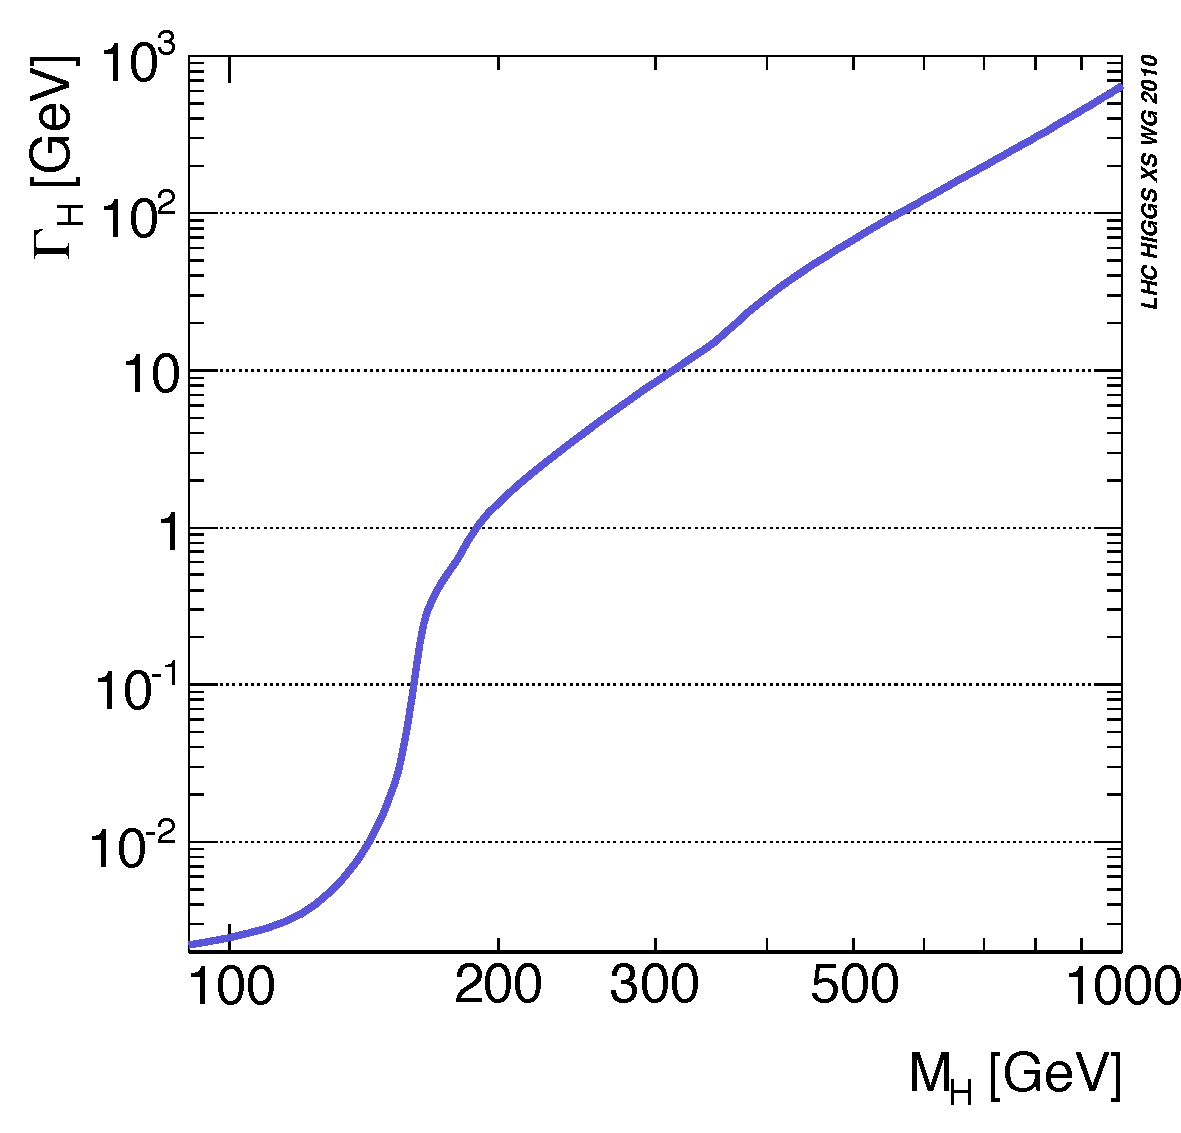
\includegraphics[width=0.46\linewidth]{{LHC_Pheno/YRHXS_BR_fig2}.pdf}
\caption[Total width of the SM Higgs boson as a function of its mass.]{Total width of the SM Higgs boson as a function of its mass\cite{Dittmaier:2011ti}.}
\label{fig:Higgs_width}
\end{center}
\end{figure}

As described in section \ref{sec:TriggerANDreconstruction}, CMS has a very fine momentum resolution for both electrons and muons. This allows CMS to accurately measure the mass and width of any new observed resonance very well, on the order of $\sim\unit{\text{few}}{\GeV}$. However, as shown in figure \ref{fig:Higgs_width} for low mass Higgs bosons the width can be quite small, on the order of $\sim\MeV$. Thus, direct measurement of the natural width of a low-mass Higgs boson will be dominated by the experimental resolution.

To overcome this, recent theoretical work has illuminated a way to measure the total width of a low-mass Higgs boson without looking at the width of the mass resonance directly. This technique relies on the ratio of the on resonance and off resonance production of the new boson. When the new boson is observed on resonance, the mass will be $m_{H} \sim \unit{125 -- 126}{\GeV}$, because this mass $m_{H} < 2m_{Z} = 2\left(\unit{91.2}{\GeV}\right)$ the Higgs boson will be real and will decay into one or more virtual Z bosons. Virtual particles are particles who's mass is not at the natural resonance, usually denoted $Z^{*}$, while real particles which have a mass at the natural resonance. For the dominant production mechanism, we have $gg \to H \to Z^{\left(*\right)}Z^{*} \to 4\ell$.

\begin{figure}
\begin{center}
\unitlength=1mm
\begin{fmffile}{ggH_ZZ_Feyn}

\begin{fmfgraph*}(40,20) 
  \fmfleft{i1,i2} \fmfright{sp1,sp2}
  \fmf{gluon,label=$g$}{i1,v1} 
  \fmf{gluon,label=$g$}{i2,v2}
  \fmf{fermion}{v1,v2,v3,v1}
  \fmffixed{(0,.5h)}{v1,v2}
  \fmf{dashes,label=$H$}{v3,v4}
  \fmffixed{(.3w,0)}{v3,v4}
  \fmf{boson,label=$Z$}{v4,sp1}
  \fmf{boson,label=$Z$}{v4,sp2}
\end{fmfgraph*}
\begin{fmfgraph*}(40,20) 
  \fmfleft{i1,i2} \fmfright{sp1,sp2,sp3,sp4}
  \fmf{gluon,label=$g$}{i1,v1} 
  \fmf{gluon,label=$g$}{i2,v2} 
  \fmffixed{(.5w,0)}{i1,v1}
  \fmffixed{(.5w,0)}{i2,v2}
  \fmf{fermion,label=$q$}{v1,v2,v3,v4,v1}
  \fmffixed{(.5w,0)}{v2,v3}
  \fmffixed{(.5w,0)}{v1,v4}
  \fmf{boson,label=$Z$}{v3,v5}
  \fmf{boson,label=$Z$}{v4,v6}
  \fmffixed{(.3w,0)}{v3,v5}
  \fmffixed{(.3w,0)}{v4,v6}
\end{fmfgraph*}

\end{fmffile}
\end{center}
\caption[(top) Feynman diagram depicting Higgs boson production through gluon-gluon fusion and subsequent decay to two Z bosons $gg \to H \to ZZ$. (bottom) Feynman diagram depicting ZZ production through gluon-gluon fusion $gg \to ZZ$. These two diagrams will interfere with eachother having an affect on the final number of events observed in the $4\ell$ final state.]{(top) Feynman diagram depicting Higgs boson production through gluon-gluon fusion and subsequent decay to two Z bosons $gg \to H \to ZZ$. (bottom) Feynman diagram depicting ZZ production through gluon-gluon fusion $gg \to ZZ$. These two diagrams will interfere with each other having an affect on the final number of events observed in the $4\ell$ final state.}
\label{fig:gg_??_ZZ_Feyn}
\end{figure}

However, the LHC will produce Higgs bosons far from this mass resonance as well. In this case, the Higgs boson will be virtual while the two Z bosons will both be  real, $gg \to H^{*} \to ZZ \to 4\ell$. In reference \cite{Kauer:2012hd} the authors point out that $\sim 10\%$ of the total Higgs boson cross section will produce Higgs bosons with a mass $m_{4\ell} > 2m_{Z}$. A plot of the Higgs boson mass shape is from this reference is shown in figure \ref{fig:Higgs_lineshape} for the ZZ and the WW final states. From this plot one can see the large fraction of the cross section that appears in this high mass window.

\begin{figure}
\begin{center}
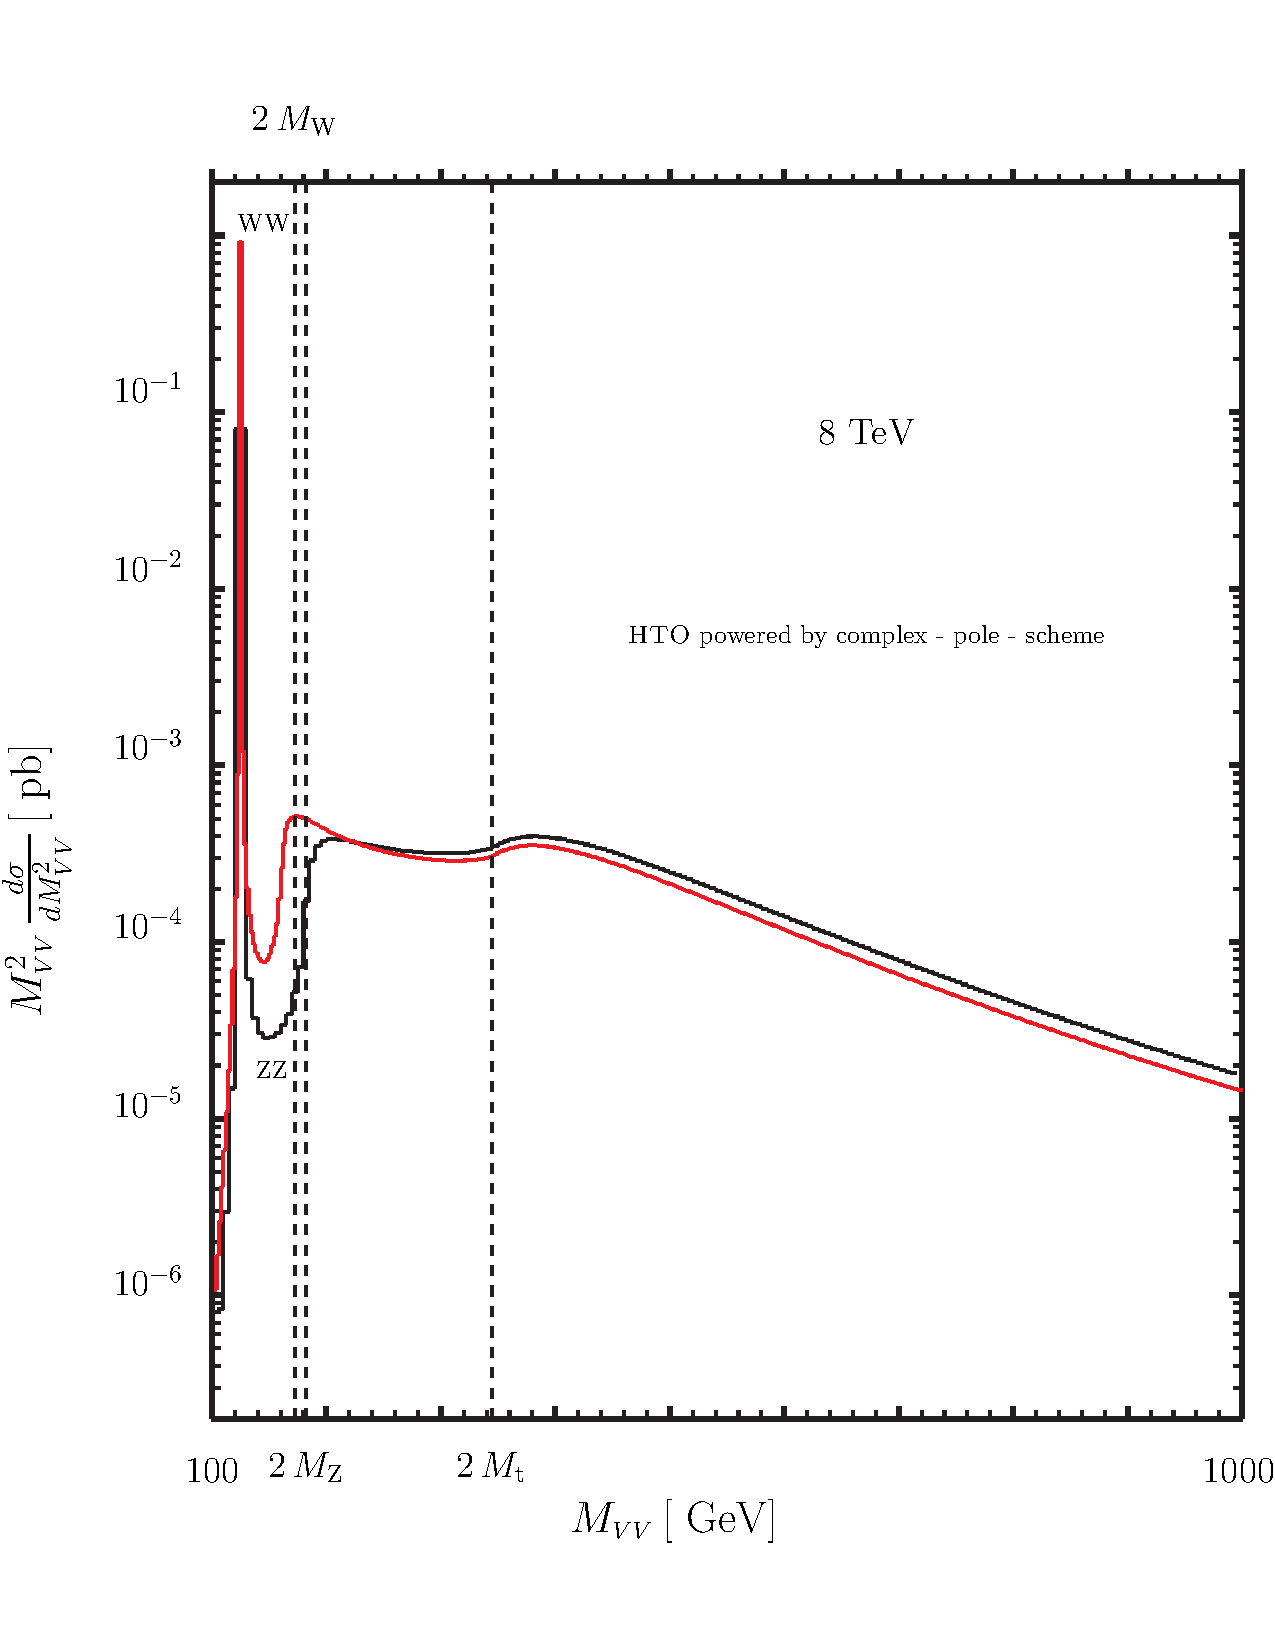
\includegraphics[width=0.46\linewidth]{{LHC_Pheno/lhzwa_fig1b}.pdf}
\caption[The NNLO ZZ (black) and WW (red) invariant mass distributions for $m_{H} = \unit{125}{\GeV}$.]{The NNLO ZZ (black) and WW (red) invariant mass distributions for $m_{H} = \unit{125}{\GeV}$\cite{Kauer:2012hd}.}
\label{fig:Higgs_lineshape}
\end{center}
\end{figure}

Following \cite{Caola:2013yja}, we can investigate the total width of the Higgs boson by comparing the on resonance and off resonance cross sections. Generally, the differential cross section of a Higgs boson produced through gluon-gluon fusion decaying into two Z bosons is given by equation \eqref{eq:diff_xsec}. Where $g_{ggH}$ is the effective coupling of the Higgs boson to gluons, $g_{HZZ}$ is the coupling of the Higgs boson to Z bosons, and $\Gamma_{H}$ is the total width of the Higgs boson. Also notice the demarcation of the observed mass of the $4\ell$ system, $m_{4\ell}$, is not necessarily the same as the Higgs boson mass $m_{H}$.

\begin{equation}
\label{eq:diff_xsec}
\frac{d\sigma_{gg \to H \to ZZ}}{d m_{4\ell}} \sim \frac{g_{ggH}^{2}g_{HZZ}^{2}}{\left(m_{4\ell}^{2} - m_{H}^{2}\right)^{2} + m_{H}^{2}\Gamma_{H}^2} 
\end{equation}

When a Higgs boson is produced on the resonance peak $m_{4\ell} \sim m_{H}$ then the mass integral can be evaluated assuming the second term in the denominator will be larger than the first. Giving the on peak cross section in equation \eqref{eq:onpeak_xsec} note that the cross section is proportional to the couplings and inversely the total width of the Higgs boson. However, if a Higgs boson is produced off of the resonance peak, specifically when $m_{4\ell} - m_{H} \gg \Gamma_{H}$, then the cross section becomes independent of the width. Shown in equation \eqref{eq:offpeak_xsec} the off peak cross section becomes proportional to the couplings but the width does not contribute.

\begin{equation}
\label{eq:onpeak_xsec}
\sigma_{gg \to H \to ZZ}^{\text{on peak}} \sim \frac{g_{ggH}^{2}g_{HZZ}^{2}}{\Gamma_{H}} 
\end{equation}

\begin{equation}
\label{eq:offpeak_xsec}
\sigma_{gg \to H \to ZZ}^{\text{off peak}} \sim g_{ggH}^{2}g_{HZZ}^{2} \sim \sigma_{gg \to H \to ZZ}^{\text{on peak}} \times \Gamma_{H}
\end{equation}

From these results we can see that the number of events that are produced on the mass resonance peak is dependent upon the total width of the new boson, while the number of events produced off peak are only dependent upon the couplings to the other SM particles. Thus, as pointed by \cite{Caola:2013yja} measuring the ratio of the on peak and off peak Higgs boson production is equivalent to measuring the total width of the new boson.

Complicating this story, is the quantum mechanical interference between the different $gg \to \ldots \to 4\ell$ processes. While this interference is present for the entire $m_{4\ell}$ range considered in this thesis, at low masses it is a very small and negligible. Above the $2m_{Z}$ mass, the interference between $gg \to ZZ \to 4\ell$ and $gg \to H^{*} \to ZZ \to 4\ell$, figure \ref{fig:gg_??_ZZ_Feyn}, processes needs to be considered. While the off peak signal contribution will scale by $\sigma_{gg \to H \to ZZ}^{\text{on peak}} \times \Gamma_{H}$ the interference between the signal and background term will scale by $\sqrt{\sigma_{gg \to H \to ZZ}^{\text{on peak}} \times \Gamma_{H}}$. 

The impact of these three terms is seen in figure \ref{fig:Higgs_sig/bkg/interf}. Here, one can clearly see the large difference between ignoring (cyan) and correctly accounting (black) for the interference in this region. Neglecting interference one would anticipate a large increase in the yield of the high mass $gg \to \ldots \to ZZ$ contribution, but since the interference between off resonance Higgs boson production and the $gg \to ZZ$ continuum background is destructive, the SM actually predicts that the high mass contribution will be lower than otherwise anticipated.

\begin{figure}
\begin{center}
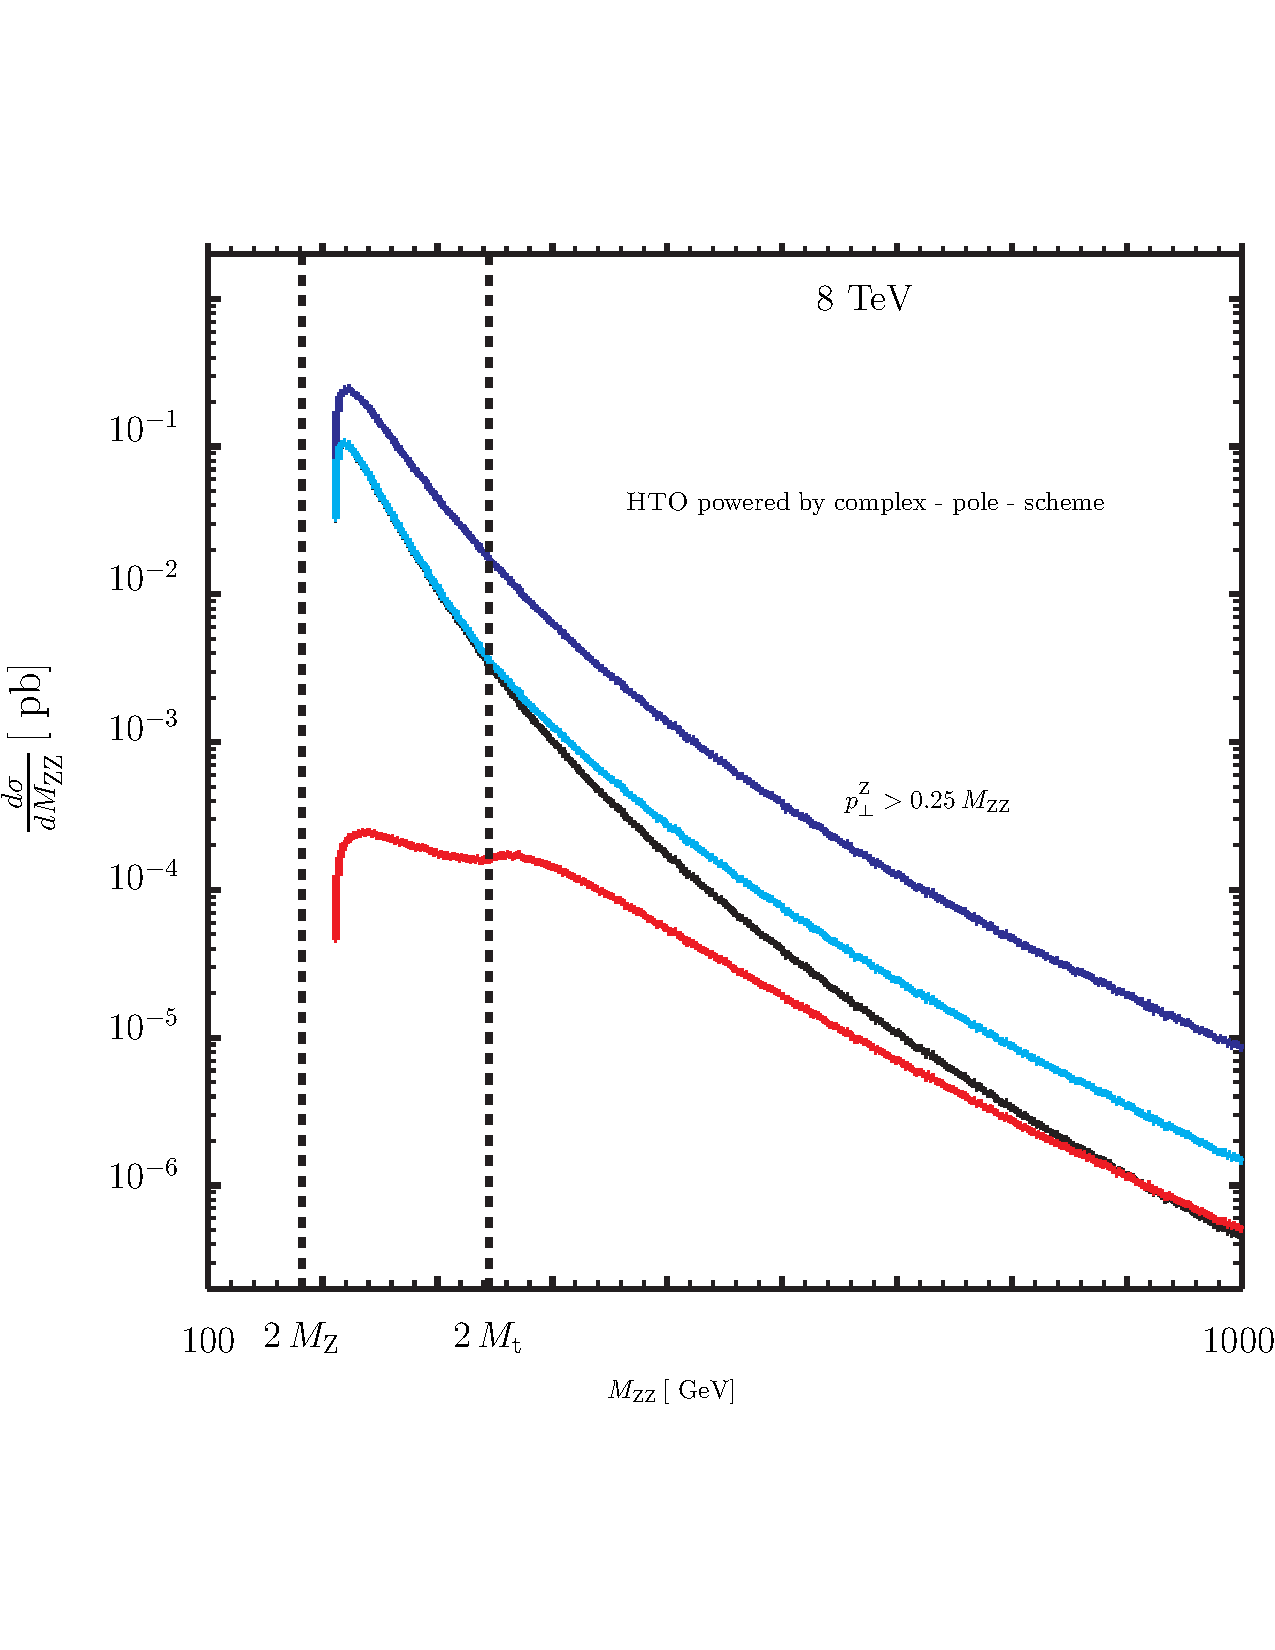
\includegraphics[width=0.46\linewidth]{{LHC_Pheno/lhzwa_fig2}.pdf}
\caption[The LO $ZZ$ invariant mass distribution $gg \to ZZ$ for $m_{H} = \unit{125}{\GeV}$. Black is the total $gg \to \ldots \to ZZ$ contribution once all interfrence effects are taken into account. Red is the $gg \to H^{*} \to ZZ$ signal only, and cyan is the $gg \to \ldots \to ZZ$ contribution ignoring the interference between the two contributions. For scale, the $q\bar{q} \to ZZ$ contribution is shown in blue.]{The LO $ZZ$ invariant mass distribution $gg \to ZZ$ for $m_{H} = \unit{125}{\GeV}$. Black is the total $gg \to \ldots \to ZZ$ contribution once all interfrence effects are taken into account. Red is the $gg \to H^{*} \to ZZ$ signal only, and cyan is the $gg \to \ldots \to ZZ$ contribution ignoring the interference between the two contributions. For scale, the $q\bar{q} \to ZZ$ contribution is shown in blue \cite{Kauer:2012hd}.}
\label{fig:Higgs_sig/bkg/interf}
\end{center}
\end{figure}

\begin{figure}
\begin{center}
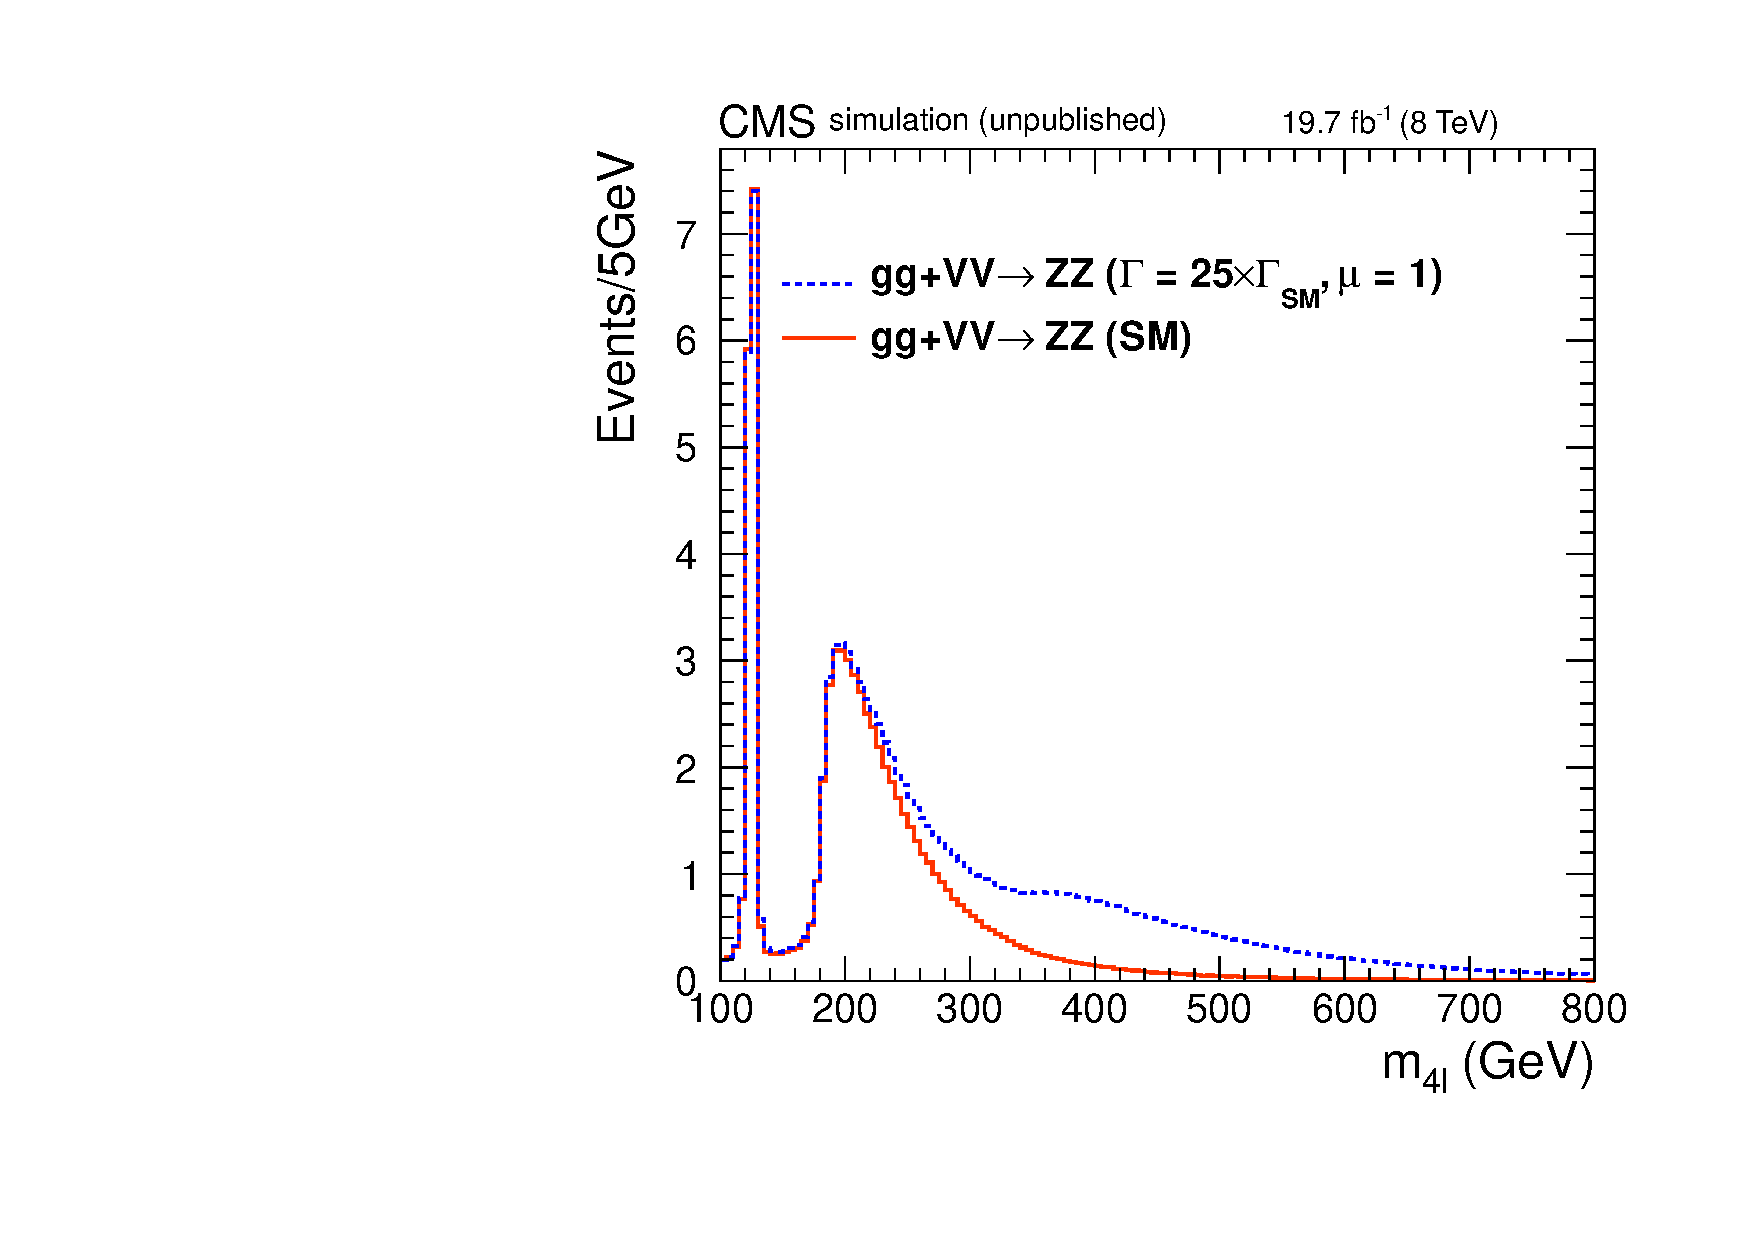
\includegraphics[width=0.46\linewidth]{{LHC_Pheno/ZZMass_100-800_SIM_20May2014}.pdf}
\caption[Distribution of the expected four-lepton reconstructed mass in full analysis mass range for the sum of the $4e$, $4\mu$, and $2e2\mu$ channels and for $gg+VV \to ZZ$ processes for a Higgs boson mass of $\unit{125.6}{\GeV}$. The expected distribution for a scenario corresponding to a scaling of the width by 25 is also shown. This illustrates the expected change in $gg+VV \to ZZ$ production when changing the Higgs boson width and at the same time constraining the peak cross section to the SM expectation.]{Distribution of the expected four-lepton reconstructed mass in full analysis mass range for the sum of the $4e$, $4\mu$, and $2e2\mu$ channels and for $gg+VV \to ZZ$ processes for a Higgs boson mass of $\unit{125.6}{\GeV}$. The expected distribution for a scenario corresponding to a scaling of the width by 25 is also shown. This illustrates the expected change in $gg+VV \to ZZ$ production when changing the Higgs boson width and at the same time constraining the peak cross section to the SM expectation \cite{Khachatryan:2014iha}.}
\label{fig:CMS_gg_ZZ}
\end{center}
\end{figure}

The resulting $m_{4\ell}$ distributions for two hypothetical bosons are shown in figure \ref{fig:CMS_gg_ZZ}, they both have the same on peak cross section but different total widths. The result is a change in the total number of events expected in the analysis. Additionally, the shape of the $m_{4\ell}$ distribution and the kinematics of the $4\ell$ will be different. A detailed description of how all of these factors are used to determine the width is given in section \ref{sec:Width_Experiment}. Also included in this image and analysis is the analogous effect for the VBF production mode.

\section{Spin and Parity of a Single-Produced Resonance}
\label{sec:Higgs_Spin_Pheno}

Using the decay rates and kinematics of a newly observed resonance one can piece together the quantum mechanical properties of the original boson. Once a new particle is observed, its spin and parity quantum numbers need to be determined. This will confirm if the new particle is the Higgs boson that was predicted or something entirely, or partially, different. Using the $H \to ZZ \to 4\ell$ decay channel is the best way to study these properties because of the small, well understood background contributions, and because all of the final state particles can be detected by CMS and have excellent precision. 

In basic terms, when a new particle is produced in a collision its spin and parity quantum numbers restrict the allowed types of interactions it can have with SM particles. This feature can be observed by investigating the kinematic distributions of the decay products or the particles produced in association with the new resonance. Of particular interest for this thesis work are the $X \to VV$ couplings (HVV). Where $V$ is any vector boson (Z, W, $\gamma$, g), and $X$ is the new resonance. When this new resonance is spin-0, we will use $H$ because the Higgs boson is predicted to be spin-0. While this vertex can be studied by using the production or decay of a new particle we will focus on the properties that can be determined from the decay products. 

When a new boson is produced it can be either spin-zero, one, or two\footnote{Unless, the resonance is actually two particles with a mass difference less than the experimental resolution.}. In this work each is considered as a possibility for a new resonance, and the differences between their kinematics are used to study and classify the newly observed boson. The relevant phenomenology for these interactions is presented below.

\subsection{Decay of a spin-zero resonance}
\label{sec:Spin0_Pheno}

The scattering amplitude describing the interaction between a spin-zero H boson and two spin-one gauge bosons $VV$ $\left(ZZ, Z\gamma, \gamma\gamma, WW \text{ or } gg\right)$ can be defined as in equation \eqref{eq:formfact-fullampl-spin0}. Where the coupling parameters $a_{i}^{VV}$ can have both real and imaginary parts and in general are form factors which can depend on the suared Lorentz invariant four-momenta of $V_{1}$ and $V_{2}$, $q_{V1}^2$ and $q_{V2}^2$. In this expression, terms of higher order than $q_{V}^2$ have been dropped in the expansion under the assumption that anomalous couplings will only have a small contribution. In this expression, we use a different notation than previous sections and label the field strength tensor of a gauge boson with momentum $q_{Vi}$ and polaraization $\epsilon_{Vi}$ with $f^{\left(i\right) \mu \nu} = \epsilon^{\mu}_{Vi}q_{Vi}^{\nu} - \epsilon^{\nu}_{Vi}q_{Vi}^{\mu}$. ${\tilde f}^{\left(i\right)}_{\mu \nu} = \frac{1}{2}\epsilon_{\mu\nu\rho\sigma}f^{\left(i\right) \rho \sigma}$ is the dual field strength tensor, and the superscript $*$ designates a complex conjugate. The masses of the Z or W boson is labeled as $m_{V1}$, while in the case of massless bosons there is no contribution from this term. To understand the impact form factor will have on the $a_{1}$ term, an energy scale $\Lambda_{1}$ for beyond-SM physics that could impact the SM scattering amplitude is also studied \cite{Anderson:2013afp}. 

\begingroup
\small
\begin{equation}
A(H\to VV) \sim
\left[ a_{1}^{VV}
+ \frac{\kappa_1^{VV}q_{V1}^2 + \kappa_2^{VV} q_{V2}^{2}}{\left(\Lambda_{1}^{VV} \right)^{2}} \right]
m_{V1}^2 \epsilon_{V1}^* \epsilon_{V2}^*
+ a_{2}^{VV}  f_{\mu \nu}^{*(1)}f^{*(2)\mu\nu}
+ a_{3}^{VV}   f^{*(1)}_{\mu \nu} {\tilde f}^{*(2)\mu\nu}
\label{eq:formfact-fullampl-spin0}
\end{equation}
\endgroup

In the SM, the tree-level contribution from $ZZ \left(WW\right)$ correspond to $a_{1}^{ZZ \left(WW\right)} \neq 0$, while the loop-induced SM contribution for $Z\gamma, \gamma\gamma, \text{ and } gg$ is $a_{2}^{VV} \neq 0$. Small SM contributions to the higher order $a_{i}$ terms can come from loop level contributions but, in general, these should be small. Additional restrictions on the allowed values for the $\kappa_{i}$ terms arise from symmetry and gauge invariance. For $ZZ$, they require $\kappa_{1}^{ZZ} = \kappa_{2}^{ZZ} = - \text{exp}\left(-i\phi_{\Lambda1}^{ZZ}\right)$ where $\phi_{\Lambda1}^{ZZ}$ is the relative phase between the $a_{1}^{ZZ}$ and $\Lambda_{1}$ terms. 

The parity conserving contribution from a pseudoscalar particle $\left( 0^{+-}, CP\text{-odd} \right)$ would be generated by the $a_{3}$ term, while a higher order scalar $\left( 0^{++}, CP\text{-even} \right)$ would be generated by $a_{2}$ or $\Lambda_{1}$ contributions. Anomalous contributions for the $\Lambda_{1}, a_{2}, \text{ or } a_{3}$ terms could be a sign of BSM physics and can in general have be complex, allowing for a relative phase between them and the SM $a_{1}$ term. To determine if these anomalous terms contribute to an observed resonance, we parameterize the contribution of one of these terms in an effective cross section fraction. These fractions are given in equation \eqref{eq:fa_definitions}, where $\sigma_{i}$ is the cross section for an $a_{i} = 1, a_{j\neq i} = 0$ particle decaying to the $2e2\mu$ final state\footnote{$\tilde{\sigma}_{\Lambda{1}}$ is the effective cross section of the process corresponding to $\Lambda_{1} = \unit{1}{\TeV}$, given in units of $\femtobarn\cdot\TeV^{4}$.}. The phases $\phi_{ai}$ are used to generalize equation \eqref{eq:formfact-fullampl-spin0} so that the anomalous contributions to be complex.

\begin{eqnarray}
f_{\Lambda1} =& \frac{\tilde{\sigma}_{\Lambda1}/\left(\Lambda_{1}\right)^{4}}{\abs{a_1}^2 \sigma_{1} + \abs{a_2}^2 \sigma_{2} + \abs{a_3}^2 \sigma_{3} + \tilde{\sigma}_{\Lambda{1}}/\left(\Lambda_{1}\right)^{4} +\ldots}, &\phi_{\Lambda1}, \nonumber \\
f_{a2} =& \frac{\abs{a_2}^2 \sigma_{2}}{\abs{a_1}^2 \sigma_{1} + \abs{a_2}^2 \sigma_{2} + \abs{a_3}^2 \sigma_{3} + \tilde{\sigma}_{\Lambda{1}}/\left(\Lambda_{1}\right)^{4} +\ldots}, &\phi_{a2} = \text{arg}\left(\frac{a_{2}}{a_{1}}\right), \\
f_{a3} =& \frac{\abs{a_3}^2 \sigma_{3}}{\abs{a_1}^2 \sigma_{1} + \abs{a_2}^2 \sigma_{2} + \abs{a_3}^2 \sigma_{3} + \tilde{\sigma}_{\Lambda{1}}/\left(\Lambda_{1}\right)^{4} +\ldots}, &\phi_{a3} = \text{arg}\left(\frac{a_{3}}{a_{1}}\right), \nonumber
\label{eq:fa_definitions}
\end{eqnarray}


These fractions are especially useful because they allow for great flexibility in the measurements. They are independent of the collider energy so they can be used to compare measurements made at different facilities, they are independent of coupling notation so can be used to translate between many different formulations for the spin-0 interactions, and they are bounded between $0$ and $1$ which allows investigation of the full phase space. 

In CMS studies of these results, analogous fractions are created for the $WW, Z\gamma, \gamma\gamma$ final states. These fractions can be combined for $ZZ$ and $WW$ under different assumptions about the relationships between the $a_{i}^{VV}$ terms. These results were a direct consequence of these studies and are left as a reference for the reader \cite{Khachatryan:2014kca}. 

\subsection{Decay of a spin-one resonance}
\label{sec:Spin1_Pheno}

In the case of a spin-one resonance, the amplitude of its interaction with a pair of massive gauge bosons, ZZ or WW, consists of two independent terms, seen in equation \eqref{eq:ampl-spin1}.

\begin{equation}
A(X_{J=1} \to VV) \sim b_{1}^{VV}  \left[ \left(\epsilon_{V1}^{*}q\right)\left(\epsilon_{V2}^{*}\epsilon_{X}\right) + \left(\epsilon_{V2}^{*}q\right)\left(\epsilon_{V1}^{*}\epsilon_{X}\right) \right] + b_{2}^{VV}  \epsilon_{\alpha\mu\nu\beta}\epsilon_{X}^{\alpha}\epsilon_{V1}^{*\mu}\epsilon_{V2}^{*\nu}{\tilde q}^{\beta}
\label{eq:ampl-spin1}
\end{equation}

Where $\epsilon_{X}$ is the polarization vector of the boson $X$ with spin one, ${q}=q_{V1}+q_{V2}$ and ${\tilde q}=q_{V1}-q_{V2}$~\cite{Gao:2010qx, Bolognesi:2012mm}. Here the $b_{1}^{VV}  \neq 0$ coupling corresponds to a vector particle, while the $b_{2}^{VV} \neq 0$ coupling corresponds to a pseudovector. The $Z\gamma$ interactions of the spin-one particle are not considered, while the $\gamma\gamma$  and $gg$ interactions are forbidden by the Landau-Yang theorem~\cite{Landau:1948kw, Yang:1950rg}, where the $gg$ case is justified by the assumption that the state $X$ is color-neutral.

The evidence for a new boson in the $ZZ$ final state will be presented in section \ref{sec:Search_Results}, similar resonances have been seen in the $H \to \gamma\gamma$ decay channel, preventing the observation from being spin-one \cite{Aad:2012tfa,Chatrchyan:2012ufa,Chatrchyan:2013lba}. In the case that the $ZZ$ resonance is different than the one seen in these references, we test if an observed boson is more consistent with spin-one or the SM predicted Higgs boson. 

Pure vector $\left(1^{+}\right)$, pseudovector $\left(1^{-}\right)$, and mixed vector-pseudovector states are tested using the fraction $f_{b2}^{VV}$ given in equation \eqref{eq:fa_definitions_spin1}. This $f_{b2}^{VV}$ parameter is a continuous unique way to define any state that is a mixture of $1^{+}$ and $1^{-}$. Where $\sigma_{bi}$ is the cross section of the process corresponding to $b_{i} = 1, b_{j\neq i} = 0$ in the $X \to ZZ \to 2e2\mu$ final state.

\begin{equation}
f_{b2}^{VV}  = \frac{\abs{b_{2}^{VV}}^2 \sigma_{b2}}{\abs{b_{1}^{VV}}^2 \sigma_{b1} + \abs{b_{2}^{VV}}^2 \sigma_{b2}},
\label{eq:fa_definitions_spin1}
\end{equation}

\subsection{Decay of a spin-two resonance}
\label{sec:Spin2_Pheno}

In the case of a general spin-two resonance, we test if a new observation is more consistent with the SM Higgs boson or a spin-two boson. The amplitude to describe the $X \to ZZ$ production is given in equation \eqref{eq:ampl-spin2-a} (This same amplitude describes the $gg \to X$ production with $m_{V} = 0$.) where $t^{\mu\nu}$ is the wavefunction of a spin-two particle $X$ given by a symmetric traceless tensor, $m_{V}$ is the mass of the considered gauge boson, and $\Lambda$ is the scale of BSM physics~\cite{Gao:2010qx, Bolognesi:2012mm}. The couplings $c_{1}^{VV}$ and $c_{5}^{VV}$ correspond to the parity-conserving interaction of a spin-two tensor with minimal gravity-like couplings. As in the spin-zero case, the couplings $c_{i}^{VV}$ are in general momentum-dependent form factors. In this analysis it is assumed that the form factors are momentum-independent constants and, thus, only the lowest $q_i^2$  order terms in the scattering amplitude are considered \cite{Khachatryan:2014kca}.



\begin{multline}
\label{eq:ampl-spin2-a}
A(X_{J=2} \to VV)  \sim \Lambda^{-1} \left [
2 c_{1}^{VV} t_{\mu \nu} f^{*1,\mu \alpha} f^{*2,\nu}_{\alpha}
+ 2 c_{2}^{VV} t_{\mu \nu} \frac{q_\alpha q_\beta }{\Lambda^2} f^{*1,\mu \alpha}  f^{*2,\nu \beta}
\right.   \\
\left.
+ c_{3}^{VV} t_{\beta \nu} \frac{{\tilde q}^\beta {\tilde q}^{\alpha}}{\Lambda^2}
 ( f^{*1,\mu \nu} f^{*2}_{\mu \alpha} + f^{*2,\mu \nu} f^{*1}_{\mu \alpha} )
 + c_{ 4}^{VV}t_{\mu \nu} \frac{{\tilde q}^{\nu} {\tilde q}^\mu}{{\Lambda^2} }  f^{*1,\alpha \beta} f^{*2}_{\alpha \beta}
\right.\\
\left. + m_{V}^2  \left (
2 c_{ 5}^{VV}  t_{\mu\nu} \epsilon_{V1}^{*\mu} \epsilon_{V2}^{*\nu}
+2 c_{ 6}^{VV}  t_{\mu \nu} \frac{{\tilde q}^\mu q_\alpha}{\Lambda^2}
\left ( \epsilon_{V1}^{*\nu} \epsilon_{V2}^{*\alpha} -
\epsilon_{V1}^{*\alpha} \epsilon_{V2}^{*\nu} \right )
+c_{ 7}^{VV} t_{\mu \nu}  \frac{{\tilde q}^\mu {\tilde q}^\nu}{\Lambda^2}  \epsilon^*_{V1} \epsilon^*_{V2}
\right)
\right.  \\
\left.
+c_{ 8}^{VV} t_{\mu \nu} \frac{{\tilde q}^{\mu} {\tilde q}^{\nu}}{\Lambda^2}
  f^{*1,\alpha \beta} {\tilde f}^{*2}_{\alpha \beta}
\right.   \\
 \left.
+  m_{V}^2  \left (
c_{ 9}^{VV} t^{\mu \alpha}
\frac{
{\tilde q}_{\alpha} \epsilon_{\mu \nu \rho \sigma} \epsilon_{V1}^{*\nu} \epsilon_{V2}^{*\rho} q^{\sigma}
}{\Lambda^2}
+c_{ 10}^{VV} t^{\mu \alpha}
\frac{
{\tilde q}_{\alpha} \epsilon_{\mu \nu \rho \sigma} q^\rho {\tilde q}^{\sigma}
\left ( \epsilon_{V1}^{*\nu}(q\epsilon_{V2}^*)+
\epsilon_{V2}^{*\nu}(q\epsilon_{V1}^*) \right )
}{\Lambda^4}
\right )
\right ]
\end{multline}


In this work, we study the ten spin-two scenarios listed in table \ref{tab:scenarios}, under the assumption that the production is via gluon-gluon fusion, $q\bar{q}$ production, or without any assumption about the production mechanism. The $q\bar{q} \to X$ couplings are parameterized in terms of $\rho_{i}$ to correctly set the polarization and defined in \cite{Khachatryan:2014kca}. The $2_m^+$ represents a massive graviton-like boson as suggested in models with warped extra dimensions \cite{Randall:1999vf, Randall:1999ee}. A modified minimal coupling model $2^+_{b}$ is also considered, where the SM fields are allowed to propagate in the bulk of the extra dimensions \cite{Agashe:2007zd}, corresponding to $c_1^{VV} \ll c_5^{VV}$. Additionally eight spin-two models with higher dimension operators are considered \cite{Khachatryan:2014kca}.

\begin{table}
\caption[List of spin-two models with the decay couplings of an exotic $X$ particle. The subscripts $m$ (minimal couplings), $h$ (couplings with higher-dimension operators), and $b$ (bulk) distinguish different scenarios.]{ List of spin-two models with the decay couplings of an exotic $X$ particle. The subscripts $m$ (minimal couplings), $h$ (couplings with higher-dimension operators), and $b$ (bulk) distinguish different scenarios \cite{Khachatryan:2014kca}. }
\centering
\begin{tabular}{cccc}
$J^{P}$ Model  &  $gg \to X$ Couplings   & $q\bar{q} \to X$ Couplings & $X \to VV$ Couplings \\

\hline

$2_m^+$  &   $c_{ 1}^{gg}\ne0$  &  $\rho_1\ne0$  & $c_{ 1}^{VV}=c_{ 5}^{VV}\ne0$     \\

$2_{h2}^+$      &   $c_{ 2}^{gg}\ne0$  &  $\rho_1\ne0$     & $c_{ 2}^{VV}\ne0$  \\

$2_{h3}^+$     &   $c_{ 3}^{gg}\ne0$  &  $\rho_1\ne0$ & $c_{ 3}^{VV}\ne0$  \\

$2_h^+$  &   $c_{ 4}^{gg}\ne0$ &  $\rho_1\ne0$ & $c_{ 4}^{VV}\ne0$  \\

$2_b^+$   &   $c_{ 1}^{gg}\ne0$  &  $\rho_1\ne0$ &  $c_{ 1}^{VV} \ll c_{ 5}^{VV}\ne0$ \\

$2_{h6}^+$  &   $c_{ 1}^{gg}\ne0$ &  $\rho_1\ne0$ & $c_{ 6}^{VV}\ne0$  \\

$2_{h7}^+$ &   $c_{ 1}^{gg}\ne0$ &  $\rho_1\ne0$ & $c_{ 7}^{VV}\ne0$ \\

$2_h^-$  &    $c_{ 8}^{gg}\ne0$ &  $\rho_2\ne0$ & $c_{ 8}^{VV}\ne0$  \\

$2_{h9}^-$ &    $c_{ 8}^{gg}\ne0$ &  $\rho_2\ne0$ & $c_{ 9}^{VV}\ne0$ \\

$2_{h10}^-$ &    $c_{ 8}^{gg}\ne0$ &  $\rho_2\ne0$ & $c_{ 10}^{VV}\ne0$ \\
\end{tabular}

\label{tab:scenarios}
\end{table}

\chapter{Conclusions}
\label{sec:Conclusions}
\chaptermark{Conclusions}

This is a reference to a previous section: ~\ref{sec:intro}

\begin{figure}
\begin{center}

\includegraphics[width=.89\linewidth]{{Conclusion/dumb-questions}.pdf}s
\caption{This is a sample figure}
\label{fig:sample}

\end{center}
\end{figure}

This is a sample citation~\cite{ATLAS:2013mla}


%\include{appendix}

%% REFERENCES

% if you use BIBTEX
\bibliographystyle{myIEEEtran}
\bibliography{thesis}

\begin{vita}
%\include{CV}
\end{vita}
\end{document}